\documentclass[a4paper,11pt, oneside]{book}
%\documentclass[a4paper,twoside,11pt,titlepage]{book}
\usepackage{listings}
\usepackage[utf8]{inputenc}
\usepackage[spanish]{babel}

% \usepackage[style=list, number=none]{glossary} %
%\usepackage{titlesec}
%\usepackage{pailatino}

\decimalpoint
\usepackage{dcolumn}
\newcolumntype{.}{D{.}{\esperiod}{-1}}
\makeatletter
\addto\shorthandsspanish{\let\esperiod\es@period@code}
\makeatother


%\usepackage[chapter]{algorithm}
\RequirePackage{verbatim}
%\RequirePackage[Glenn]{fncychap}
\usepackage{fancyhdr}
\usepackage{graphicx}
\usepackage{afterpage}

\usepackage{longtable}

\usepackage[pdfborder={000}]{hyperref} %referencia

\usepackage{amsthm}
\usepackage{amsmath}
\usepackage{amssymb}

\usepackage{array}
\usepackage{eurosym}
\usepackage{subfig}
% ********************************************************************
% Re-usable information
% ********************************************************************
\newcommand{\myTitle}{Sistema de adaptación motora con entorno de realidad virtual\xspace}
\newcommand{\myDegree}{Grado en ...\xspace}
\newcommand{\myName}{Celia Arias Martínez (alumno)\xspace}
\newcommand{\myProf}{Nombre Apllido1 Apellido2 (tutor1)\xspace}
\newcommand{\myOtherProf}{Nombre Apllido1 Apellido2 (tutor2)\xspace}
%\newcommand{\mySupervisor}{Put name here\xspace}
\newcommand{\myFaculty}{Escuela Técnica Superior de Ingenierías Informática y de
Telecomunicación\xspace}
\newcommand{\myFacultyShort}{E.T.S. de Ingenierías Informática y de
Telecomunicación\xspace}
\newcommand{\myDepartment}{Departamento de ...\xspace}
\newcommand{\myUni}{\protect{Universidad de Granada}\xspace}
\newcommand{\myLocation}{Granada\xspace}
\newcommand{\myTime}{\today\xspace}
\newcommand{\myVersion}{Version 0.1\xspace}



\hypersetup{
pdfauthor = {\myName (email (en) ugr (punto) es)},
pdftitle = {\myTitle},
pdfsubject = {},
pdfkeywords = {palabra_clave1, palabra_clave2, palabra_clave3, ...},
pdfcreator = {LaTeX con el paquete ....},
pdfproducer = {pdflatex}
}

%\hyphenation{}


%\usepackage{doxygen/doxygen}
%\usepackage{pdfpages}
\usepackage{url}
\usepackage{colortbl,longtable}
\usepackage[stable]{footmisc}
%\usepackage{index}

%\makeindex
%\usepackage[style=long, cols=2,border=plain,toc=true,number=none]{glossary}
% \makeglossary

% Definición de comandos que me son tiles:
%\renewcommand{\indexname}{Índice alfabético}
%\renewcommand{\glossaryname}{Glosario}

\pagestyle{fancy}
\fancyhf{}
\fancyhead[LO]{\leftmark}
\fancyhead[RE]{\rightmark}
\fancyhead[RO,LE]{\textbf{\thepage}}
\renewcommand{\chaptermark}[1]{}



\setlength{\headheight}{1.5\headheight}

\newcommand{\HRule}{\rule{\linewidth}{0.5mm}}
%Definimos los tipos teorema, ejemplo y definición podremos usar estos tipos
%simplemente poniendo \begin{teorema} \end{teorema} ...
\newtheorem{teorema}{Teorema}[chapter]
\newtheorem{ejemplo}{Ejemplo}[chapter]
\newtheorem{definicion}{Definición}[chapter]

\definecolor{gray97}{gray}{.97}
\definecolor{gray75}{gray}{.75}
\definecolor{gray45}{gray}{.45}
\definecolor{gray30}{gray}{.94}

\lstset{ frame=Ltb,
     framerule=0.5pt,
     aboveskip=0.5cm,
     framextopmargin=3pt,
     framexbottommargin=3pt,
     framexleftmargin=0.1cm,
     framesep=0pt,
     rulesep=.4pt,
     backgroundcolor=\color{gray97},
     rulesepcolor=\color{black},
     %
     stringstyle=\ttfamily,
     showstringspaces = false,
     basicstyle=\scriptsize\ttfamily,
     commentstyle=\color{gray45},
     keywordstyle=\bfseries,
     %
     numbers=left,
     numbersep=6pt,
     numberstyle=\tiny,
     numberfirstline = false,
     breaklines=true,
   }
 
% minimizar fragmentado de listados
\lstnewenvironment{listing}[1][]
   {\lstset{#1}\pagebreak[0]}{\pagebreak[0]}

\lstdefinestyle{CodigoC}
   {
	basicstyle=\scriptsize,
	frame=single,
	language=C,
	numbers=left
   }
\lstdefinestyle{CodigoC++}
   {
	basicstyle=\small,
	frame=single,
	backgroundcolor=\color{gray30},
	language=C++,
	numbers=left
   }

 
\lstdefinestyle{Consola}
   {basicstyle=\scriptsize\bf\ttfamily,
    backgroundcolor=\color{gray30},
    frame=single,
    numbers=none
   }


\newcommand{\bigrule}{\titlerule[0.5mm]}


%Para conseguir que en las páginas en blanco no ponga cabecerass
\makeatletter
\def\clearpage{%
  \ifvmode
    \ifnum \@dbltopnum =\m@ne
      \ifdim \pagetotal <\topskip
        \hbox{}
      \fi
    \fi
  \fi
  \newpage
  \thispagestyle{empty}
  \write\m@ne{}
  \vbox{}
  \penalty -\@Mi
}
\makeatother

\graphicspath{ {imagenes/} }

\usepackage{pdfpages}

\newtheorem{defi}{Definición}

\newtheorem{prop}{Proposición}


\begin{document}
\begin{titlepage}
 
 
\newlength{\centeroffset}
\setlength{\centeroffset}{-0.5\oddsidemargin}
\addtolength{\centeroffset}{0.5\evensidemargin}
\thispagestyle{empty}

\noindent\hspace*{\centeroffset}\begin{minipage}{\textwidth}

\centering

\includegraphics[width=0.9\textwidth]{imagenes/logo_ugr.jpg}\\[1.4cm]

\textsc{ \Large TRABAJO FIN DE GRADO\\[0.2cm]}
\textsc{ INGENIERÍA EN ...}\\[1cm]
% Upper part of the page
% 
% Title
{\Huge\bfseries Titulo del Proyecto\\
}
\noindent\rule[-1ex]{\textwidth}{3pt}\\[3.5ex]
{\large\bfseries Subtitulo del Proyecto}
\end{minipage}

\vspace{2.5cm}
\noindent\hspace*{\centeroffset}\begin{minipage}{\textwidth}
\centering

\textbf{Autor}\\ {Nombre Apellido1 Apellido2 (alumno)}\\[2.5ex]
\textbf{Directores}\\
{Nombre Apellido1 Apellido2 (tutor1)\\
Nombre Apellido1 Apellido2 (tutor2)}\\[2cm]

\includegraphics[width=0.3\textwidth]{imagenes/etsiit_logo.png}\\[0.1cm]
\textsc{Escuela Técnica Superior de Ingenierías Informática y de Telecomunicación}\\
\textsc{---}\\
Granada, mes de 201
\end{minipage}
%\addtolength{\textwidth}{\centeroffset}
%\vspace{\stretch{2}}
\end{titlepage}



\chapter*{}
%\thispagestyle{empty}
%\cleardoublepage

%\thispagestyle{empty}

\begin{titlepage}
 
 
\setlength{\centeroffset}{-0.5\oddsidemargin}
\addtolength{\centeroffset}{0.5\evensidemargin}
\thispagestyle{empty}

\noindent\hspace*{\centeroffset}\begin{minipage}{\textwidth}

\centering
%
\includegraphics[width=0.9\textwidth]{imagenes/logo_ugr.jpg}\\[1.4cm]

%\textsc{ \Large PROYECTO FIN DE CARRERA\\[0.2cm]}
%\textsc{ INGENIERÍA EN INFORMÁTICA}\\[1cm]
% Upper part of the page
% 

 \vspace{3.3cm}

%si el proyecto tiene logo poner aquí

\includegraphics{imagenes/logo.png} 
 \vspace{0.5cm}

% Title

{\Huge\bfseries Sistema de adaptación motora con entorno de realidad virtual\\
}
%\noindent\rule[-1ex]{\textwidth}{3pt}\\[3.5ex]
%{\large\bfseries Subtítulo del proyecto.\\[4cm]}
\end{minipage}

\vspace{2.5cm}
\noindent\hspace*{\centeroffset}\begin{minipage}{\textwidth}
\centering

\textbf{Autor}\\ {Nombre Apellido1 Apellido2 (alumno)}\\[2.5ex]
\textbf{Directores}\\
{Nombre Apellido1 Apellido2 (tutor1)\\
Nombre Apellido1 Apellido2 (tutor2)}\\[2cm]
%
\includegraphics[width=0.15\textwidth]{imagenes/tstc.png}\\[0.1cm]
%\textsc{Departamento de Teoría de la Señal, Telemática y Comunicaciones}\\
%\textsc{---}\\
%Granada, mes de 201
\end{minipage}
%\addtolength{\textwidth}{\centeroffset}
\vspace{\stretch{2}}

 
\end{titlepage}






\cleardoublepage
\thispagestyle{empty}

\begin{center}
{\large\bfseries Título del Proyecto: Subtítulo del proyecto}\\
\end{center}
\begin{center}
Nombre Apellido1 Apellido2 (alumno)\\
\end{center}

%\vspace{0.7cm}
\noindent{\textbf{Palabras clave}: palabra\_clave1, palabra\_clave2, palabra\_clave3, ......}\\

\vspace{0.7cm}
\noindent{\textbf{Resumen}}\\

Poner aquí el resumen.
\cleardoublepage


\thispagestyle{empty}


\begin{center}
{\large\bfseries Project Title: Project Subtitle}\\
\end{center}
\begin{center}
First name, Family name (student)\\
\end{center}

%\vspace{0.7cm}
\noindent{\textbf{Keywords}: Keyword1, Keyword2, Keyword3, ....}\\

\vspace{0.7cm}
\noindent{\textbf{Abstract}}\\

Write here the abstract in English.

\chapter*{}
\thispagestyle{empty}

\noindent\rule[-1ex]{\textwidth}{2pt}\\[4.5ex]

Yo, \textbf{Nombre Apellido1 Apellido2}, alumno de la titulación TITULACIÓN de la \textbf{Escuela Técnica Superior
de Ingenierías Informática y de Telecomunicación de la Universidad de Granada}, con DNI XXXXXXXXX, autorizo la
ubicación de la siguiente copia de mi Trabajo Fin de Grado en la biblioteca del centro para que pueda ser
consultada por las personas que lo deseen.

\vspace{6cm}

\noindent Fdo: Nombre Apellido1 Apellido2

\vspace{2cm}

\begin{flushright}
Granada a X de mes de 201 .
\end{flushright}


\chapter*{}
\thispagestyle{empty}

\noindent\rule[-1ex]{\textwidth}{2pt}\\[4.5ex]

D. \textbf{Nombre Apellido1 Apellido2 (tutor1)}, Profesor del Área de XXXX del Departamento YYYY de la Universidad de Granada.

\vspace{0.5cm}

D. \textbf{Nombre Apellido1 Apellido2 (tutor2)}, Profesor del Área de XXXX del Departamento YYYY de la Universidad de Granada.


\vspace{0.5cm}

\textbf{Informan:}

\vspace{0.5cm}

Que el presente trabajo, titulado \textit{\textbf{Título del proyecto, Subtítulo del proyecto}},
ha sido realizado bajo su supervisión por \textbf{Nombre Apellido1 Apellido2 (alumno)}, y autorizamos la defensa de dicho trabajo ante el tribunal
que corresponda.

\vspace{0.5cm}

Y para que conste, expiden y firman el presente informe en Granada a X de mes de 201 .

\vspace{1cm}

\textbf{Los directores:}

\vspace{5cm}

\noindent \textbf{Nombre Apellido1 Apellido2 (tutor1) \ \ \ \ \ Nombre Apellido1 Apellido2 (tutor2)}

\chapter*{Agradecimientos}
\thispagestyle{empty}

       \vspace{1cm}


Poner aquí agradecimientos...


%\frontmatter
%\tableofcontents
%\listoffigures
%\listoftables
%
%\mainmatter
%\setlength{\parskip}{5pt}

%\input{capitulos/01_Introduccion}
%
%\input{capitulos/02_EspecificacionRequisitos}
%
%\input{capitulos/03_Planificacion}
%
%\input{capitulos/04_Analisis}
%
%\input{capitulos/05_Diseno}
%
%\input{capitulos/06_Implementacion}
%
%\input{capitulos/07_Pruebas}
%
%\input{capitulos/08_Conclusiones}
%
%%\chapter{Conclusiones y Trabajos Futuros}
%
%
%%\nocite{*}
%\bibliography{bibliografia/bibliografia}\addcontentsline{toc}{chapter}{Bibliografía}
%\bibliographystyle{miunsrturl}
%
%\appendix
%\input{apendices/manual_usuario/manual_usuario}
%%\input{apendices/paper/paper}
%\input{glosario/entradas_glosario}
% \addcontentsline{toc}{chapter}{Glosario}
% \printglossary
\tableofcontents

\chapter{Introducción}

\section{Contexto del proyecto}

El cerebelo, una estructura ubicada en la base del cerebro, ha sido ampliamente estudiado en relación con el aprendizaje y el control de movimientos. Experimentos científicos han revelado su papel fundamental en la adquisición de habilidades motoras y en la coordinación precisa de los movimientos, mostrando que, los individuos con daños en el cerebelo presentan dificultades para adaptarse a nuevos patrones de movimiento o para realizar ajustes precisos en la fuerza y la dirección de sus movimientos.

La realidad virtual ha sido utilizada como una herramienta para investigar la función del cerebelo en la percepción espacial, la coordinación motora y el aprendizaje de movimientos. En los experimentos los participantes son expuestos a entornos virtuales que simulan situaciones específicas -manipulación de objetos virtuales, laberintos, simulaciones de deportes, etc. Durante estos experimentos se analiza la precisión de los movimientos de los individuos, la percepción espacial y la diferencia entre la capacidad de adaptación de los individuos sanos y los individuos con lesiones en el cerebelo.

Podemos definir la realidad virtual como una tecnología que permite a los usuarios sumergirse en un entorno generado por computadora que simula la realidad física o crea un mundo virtual completamente nuevo. Los dispositivos de realidad virtual rastrean los movimientos de la cabeza y, en algunos casos, también los movimientos de las manos y del cuerpo, para permitir que los usuarios exploren y manipulen el entorno virtual de manera natural. 

Algunos de los dispositivos de realidad virtual son: los cascos de realidad virtual (o Head Mounted Display), que se colocan en la cabeza y cubren los ojos del usuario, ofreciendo una experiencia inmersiva al mostrar imágenes estereoscópicas en 3D; los simuladores de realidad virtual, como los simuladores de vuelo, donde la inmersión es completa y reconoce todos los movimientos de nuestro cuerpo; los dispositivos hápticos que simulan respuestas táctiles acordes con las imágenes que vemos, etc.

Dentro de los experimentos relacionados con el estudio de los movimientos asociados al cerebelo utilizando estos dispositivos podemos encontrar los siguientes artículos:


En \textit{''The vestibulo-ocular reflex and angular displacement perception in darkness in humans: adaptation to a virtual environment''} los autores utilizan gafas de realidad virtual para medir la respuesta vestíbulo-ocular de los sujetos en un escenario de oscuridad. El reflejo vestíbulo-ocular (RVO) es un mecanismo que coordina los movimientos oculares con los movimientos de la cabeza para mantener la estabilidad visual. En este caso en el entorno visual se generaron movimientos de rotación y se midieron los movimientos oculares de los participantes para estudiar si la falta de señales visuales influye en la precisión de la percepción espacial.


En \textit{''Assessing Saccadic Eye Movements
	With Head-Mounted Display Virtual
	Reality Technology''}. En este artículo los autores utilizan el dispositivo HTC VIVE Pro Eye (unas gafas de realidad virtual con eye tracking) para estudiar los movimientos oculares sacádicos, es decir, los desplazamientos rápidos de la fijación de un punto a otro del campo visual. 
	

En \textit{''Cerebellar Contributions to Reach Adaptation and Learning Sensory Consequences of Action''} los autores utilizan un brazo robot que se proyecta en una pantalla, mientras que se oculta la visión del propio brazo. Se utiliza para estudiar los procesos de aprendizaje de dos tipos diferentes de movimientos: los de modelo directo (se asocia un comando motor con sus consecuencias sensoriales) y los de modelo inverso (se asocia un objetivo con el comando motor necesario para alcanzarlo).


Los resultados evidencian que la tecnología de realidad virtual proporciona un entorno controlado y estandarizado para estudiar los movimientos asociados con el cerebelo, facilitando la comparación entre los participantes y la realización de análisis cuantitativos. Sin embargo, la mayoría de los experimentos realizados hasta el momento se apoyan en el uso de gafas de realidad virtual. Nuestro objetivo en este proyecto es comprobar si los dispositivos hápticos ofrecen las capacidades necesarias para llevar a cabo este tipo de experimentos.

\section{Objetivos}

Dentro de los objetivos del proyecto vamos a distinguir entre los objetivos técnicos, relacionados con el estudio de cómo los dispositivos hápticos podrían usarse en el diseño de experimentos sobre la relación del cerebelo con determinados tipos de movimientos, y los objetivos didácticos, relacionados con el aprendizaje de cómo debe llevarse a cabo una experimentación científica, y en concreto con el desarrollo de una aplicación que utilice un dispositivo háptico.

\begin{itemize}
	\item Objetivos técnicos:
	\begin{itemize}
	\item Estudiar cómo los dispositivos hápticos, en concreto el dispositivo System3D Touch, pueden ser usados para el estudio de movimientos balísticos controlados por el cerebelo.
	
	\item Estudiar si los datos obtenidos con System3D Touch son lo suficientemente precisos para que pudiera utilizarse en este tipo de experimentos.
	
	\item Estudiar qué tipo de datos podemos obtener a través de los experimentos realizados con System3D Touch, así cómo qué interpretaciones podemos elaborar utilizando dichos datos.

	\end{itemize}
	\item Objetivos didácticos:
	\begin{itemize}
		\item Aprender a usar el dispositivo System3D Touch.
		\item Aprender a utilizar alguna de las APIs de System3D Touch y ser capaz de desarrollar una aplicación que utilice System3D Touch.
		\item Comprender en profundidad los conceptos relacionados con los cambios de sistemas de coordenadas, y su relación con el espacio afín y el proyectivo. 
		\item Ser capaz de plantear y llevar a cabo un experimento en el que podamos observar los resultados de diferentes sujetos.
		\item Realizar un análisis de los datos obtenidos utilizando python.

	\end{itemize}
\end{itemize}


\section{Fases del proyecto}
El proyecto ha sido desarrollado en cuatro fases: planificación del experimento, desarrollo de la aplicación, obtención de resultados mediante la utilización de la aplicación en distintos usuarios y análisis de los resultados obtenidos. 
\begin{enumerate}
	\item Planificación del experimento: en esta etapa se definió el experimento que íbamos a realizar, teniendo en cuenta contenido, fases de las que consistiría y grupos de población en los que íbamos a realizarlo.
	\item Desarrollo de la aplicación: esta etapa se dedicó a desarrollar la aplicación que se utilizaría después para la realización de los experimentos. A su vez esta etapa se dividió en tres subetapas:
	\begin{enumerate}
		\item Instalación de los paquetes necesarios para utilizar el dispositivo System 3D Touch.
		\item Desarrollo del código necesario para implementar la aplicación.
		\item Revisión del código para utilizar los parámetros idóneos. Esta etapa se realizó una vez acabada la primera prueba de realización del experimento.
	\end{enumerate}
	\item Obtención de resultados: en esta etapa distintos usuarios llevaron a cabo el experimento planeado, haciendo uso de la aplicación implementada en la fase anterior.
	A su vez esta etapa se dividió en dos:
	\begin{enumerate}
		\item Fase de prueba, en la que se eligió a un primer grupo de sujetos para la realización del experimento, cada uno con un set de parámetros diferentes. Esta fase nos ayudó a decidir los parámetros que queríamos utilizar finalmente.
		\item Fase final, en la que se eligió a un segundo grupo de sujetos (ninguno de los cuales había participado en la fase de prueba) y se realizó el experimento con los parámetros que finalmente habíamos elegido.
		Estos resultados fueron los que se utilizaron para fase Análisis de los resultados.
	\end{enumerate}
		
	\item Análisis de los resultados: en esta etapa analizamos las graficas obtenidas con los datos de la etapa anterior, para así obtener conclusiones del experimento.
\end{enumerate}

Por tanto podemos decir que el proyecto ha seguido un modelo de ciclo de vida en cascada, en el que en algunas etapas ha habido realimentación, dado que la información conseguida en algunas etapas nos ha servido para modificar etapas anteriores. Este proceso puede verse reflejado en la Figura:

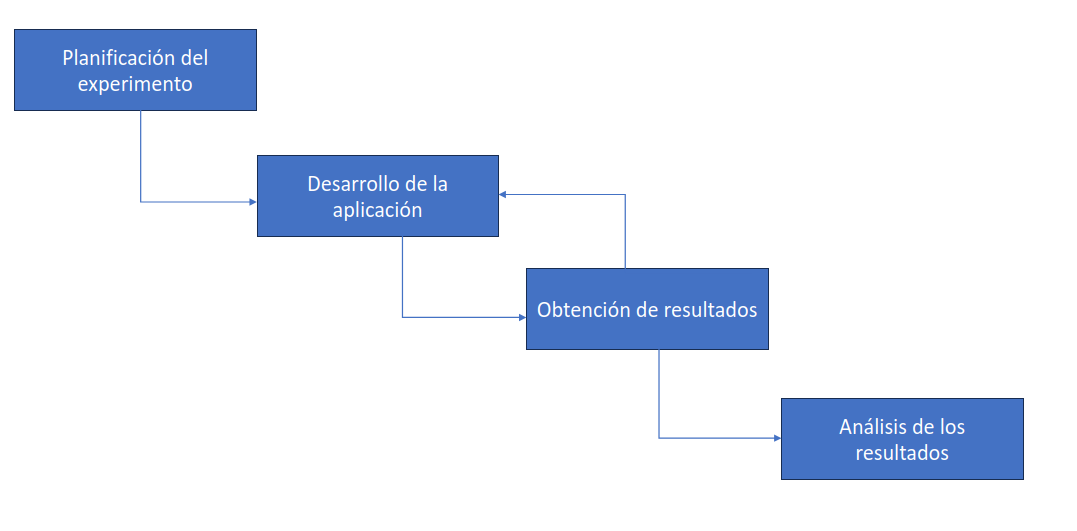
\includegraphics[scale=0.3]{diagrama-fases}

Por otro lado la toma de decisiones en las distintas fases se ha llevado a cabo mediante reuniones regulares (telemáticas y presenciales) y la comunicación mediante correo electrónico.

\section{Planificación del proyecto}
El proyecto fue pensado para ser desarrollado entre los meses de septiembre y junio. La planificacion inicial fue:
\begin{itemize}
	\item Septiembre: planificación del experimento.
	\item De octubre a diciembre: desarrollo de la aplicación.
	\item De enero a marzo: obtención de resultados
	\item De marzo hasta mayo: análisis de resultados y redacción de la memoria.
\end{itemize}

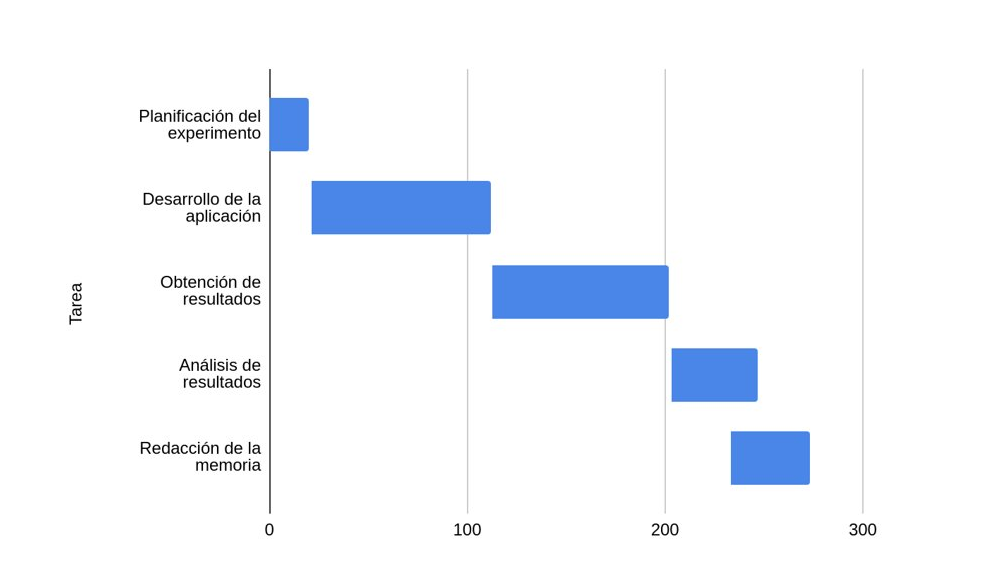
\includegraphics[scale=0.4]{gantt}

La etapa mas larga fue de la del desarrollo de la aplicación pues es la que sustentaba todo el trabajo que podíamos realizar después. Por eso fue la que más carga de trabajo acumuló, y a la que más horas se le dedicó.



El reparto de horas respecto a las distintas tareas fue:
\begin{itemize}
	\item Planificación del experimento: 10 horas. 
	\item Desarrollo de la aplicación:
		\begin{itemize}
			\item Instalación del software y familarización con el: 35 horas
			\item Desarrollo del programa: 60 horas
		\end{itemize}
	\item Obtención de resultados: 40 horas
	\item Análisis de resultados:
	\item Total de horas: 
\end{itemize}

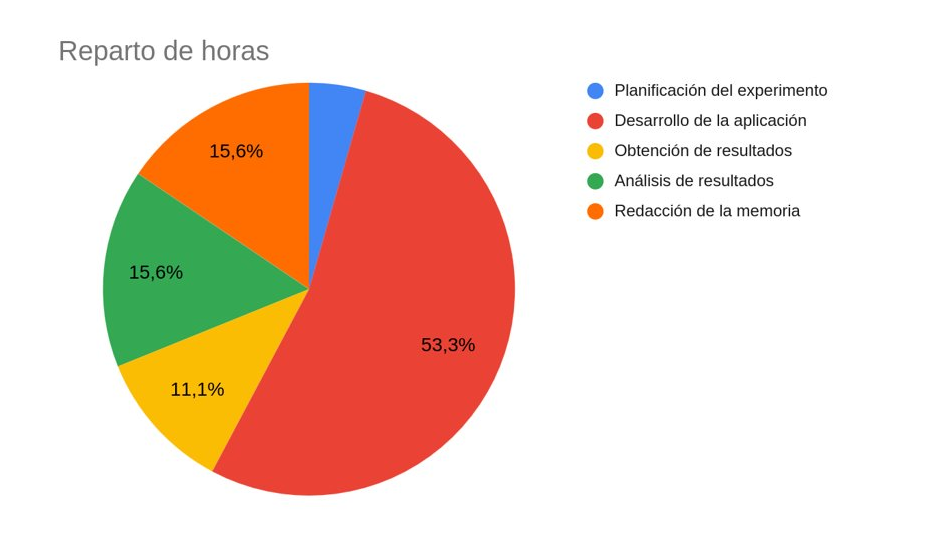
\includegraphics[scale=0.4]{horas}


Por tanto, teniendo en cuenta que el salario medio de un profesional junior es de 11\euro /hora, el coste en personal seria de ....

Por otro lado tenemos que añadir el coste del dispositivo System3D Touch: 

Por último, dado la necesidad de realizar el experimento en individuos externos al proyecto y teniendo en cuenta la duración media de este (45 minutos) decidimos ofrecer una compensación material a los individuos que se presentaran voluntarios, en concepto de coste de transporte. La compensación la hemos fijado en 5 euros por persona, y dado que necesitamos -- voluntarios ( -- para la fase de prueba y -- para la fase final), el coste adicional será de --- euros.

Por tanto el presupuesto final fue de -- euros, repartido como puede verse en la siguiente figura:

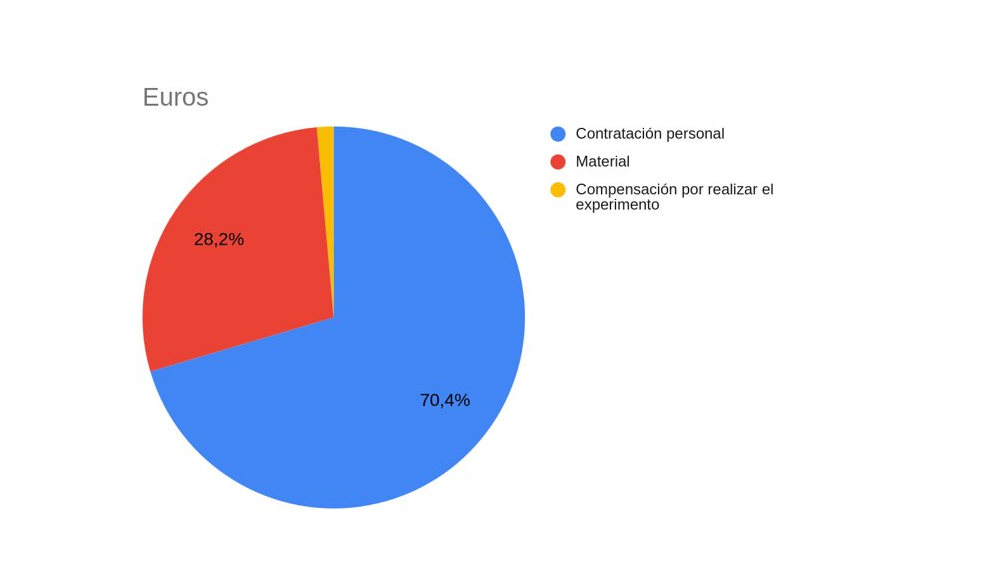
\includegraphics[scale=0.4]{coste}

\section{Material}

\subsection{Touch}

Touch ha sido el dispositivo sobre el que se ha hecho la aplicación, y que se ha utilizado posteriormente para la realización del experimento.

Es un dispositivo háptico desarrollado por la empresa 3D Systems. Los dispositivos hápticos simulan respuestas táctiles, mediante las cuales podemos percibir objetos tridimensionales en un ambiente de realidad virtual.
Según la propia documentación de 3D Systems: \textit{''Touch es un dispositivo motorizado que aplica retroalimentación de fuerza a la mano del usuario, lo que le permite sentir objetos virtuales y producir sensaciones táctiles reales a medida que el usuario manipula los objetos 3D en la pantalla''}. Touch es utilizado en aplicaciones de control robótico, rehabilitación, medicina y cirugía, etc.

\subsubsection{Especificaciones técnicas}
\renewcommand{\arraystretch}{1.3}
\begin{center}
	\begin{tabular}{ |m{6cm}|m{6cm}| } 
		\hline
		\textbf{Área de trabajo y retroalimentación de fuerza} & 431 ancho. × 348 altura. × 165 profundidad. mm \\ 
		\hline
		\textbf{Tamaño (espacio físico que la base del dispositivo ocupa en una superficie)} & 168 ancho x 203 profundidad mm  \\ 
		\hline
		\textbf{Peso (solo dispositivo)} & ~1,42 kg  \\ 
		\hline
		\textbf{Rango de movimiento} & Movimiento de la mano con giro de la muñeca \\
		\hline
		\textbf{Resolución de la posición nominal} & ~ 0,055 mm \\
		\hline
		\textbf{Fricción de accionamiento trasero} & $< 0,26$ N \\
		\hline
		\textbf{Fuerza de esfuerzo máxima (en la posición nominal de los brazos ortogonales)} & 3,3 N \\
		\hline
		\textbf{Fuerza de esfuerzo continua (24 h)} & $>0,88$ N \\
		\hline
		\textbf{Rigidez} & \parbox[t]{11em}{Eje X $> 1,26$ N/mm \\ Eje Y $> 2,31$ N/mm  \\ Eje Z $> 1,02$ N/mm} \\
		\hline
		\textbf{Inercia (masa aparente en la punta)} & $\backsim45$ g \\
		\hline
		\textbf{Retroalimentación de fuerza} & x, y, z \\
		\hline
		\textbf{Detección de posición} & x, y, z (codificadores digitales) \\
		\hline
		\textbf{Cardán de lápiz} & Inclinación, giro, dirección (± 5 \% de potenciómetros de linealidad) \\
		\hline
		\textbf{Interfaz} & USB 2.0/puerto 3.0 o hub USB que admita USB 2.0/3.0.
		Frecuencia de actualización 1 KHz \\
		\hline
	\end{tabular}
\end{center}


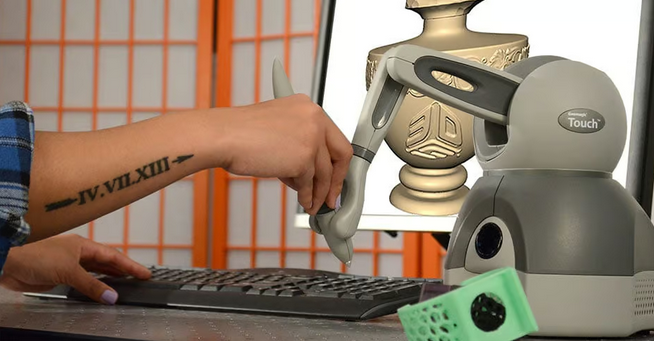
\includegraphics[scale=0.5]{touch}

\subsection{OpenHaptics}

OpenHaptics es un software para desarrolladores hápticos que permite crear aplicaciones que utilicen Touch. Está basado en la API de OpenGL y está disponible para Windows de 64 bits 10 y 11 y para Linux. 

OpenHaptics incluye varias APIs desarrolladas en C++, y viene con varios ejemplos de aplicaciones, una guía de usuario y dos guías para los desarrolladores: OpenHaptics Programmers Guide y OpenHaptics API Reference Guide. 




\chapter{Fundamentos matemáticos}

Un proceso clave a la hora de desarrollar la aplicación ha sido trasladar las coordenadas obtenidas a través del dispositivo Touch a la pantalla del ordenador. De esta forma hemos podido obtener las trayectorias que cada sujeto ha realizado tal y como ellos las han visto reflejadas en la pantalla. 

Para explicar el proceso de transformación de coordenadas vamos a introducir previamente algunos conceptos matemáticos que necesitaremos después. Las transformaciones que aplicaremos incluyen traslaciones, rotaciones, escalados y proyecciones. Para estudiar estos movimientos introduciremos dos conceptos matemáticos muy importantes: las transformaciones afines y las proyecciones. Estos conceptos se basan en el estudio de la Geometría afín y proyectiva, que a su vez tienen una base en el Álgebra lineal. 


\section{Álgebra lineal, Geometría afín y Geometría Proyectiva}
% https://www.emis.de/journals/DM/v14-2/art6.pdf
Podemos encontrar los primeros antecedentes del álgebra lineal en el libro del Cálculo, escrito por el sacerdote egipcio Ahmés hacia el año 1650 a.C. En él se describen algunos problemas relacionados con la agricultura, que involucran sistemas de ecuaciones de primer grado. Los matemáticos babilonios, griegos, chinos e islámicos siguieron estudiando estos tipos de problemas, pero no fue hasta el siglo  XIX cuando Hamilton, Cayley y Grassmann introdujeron las nociones de vector y espacio vectorial, desarrollando gran parte de los conceptos que estudiaremos en este capítulo. En el año 1850 Sylvester introdujo el término matriz, y en 1858, en su libro \textit{Memoir on the theory of matrices}, Cayley utiliza las matrices para explicar las transformaciones lineales.

La geometría afín surge con Euler y se consolida con Klein en 1872 mediante el Programa de Erlangen, un programa de investigación con el objetivo de proponer una solución a los problemas que la Geometría se enfrentaba en ese momento. Klein define la geometría afín como una generalización de la geometria asociada al álgebra lineal. El espacio afín se construye sobre el espacio vectorial, con la diferencia de que no tenemos un vector de referencia, lo que nos dará la capacidad de hacer traslaciones. A su vez Klein engloba la geometría afín dentro de la geometría proyectiva.

En el Programa de Erlangen, Klein también introduce el concepto de Grupo (un conjunto en el que hay definido una operación que cumple ciertas propiedades) en la Geometría. Para Klein cada Geometría es el estudio de las propiedades que no cambian al aplicar un tipo de transformaciones. Por ejemplo, el algebra lineal estudia las propiedades de los espacios al aplicar movimientos lineales (escalados, rotaciones sobre el origen), la geometría afín al aplicar movimientos afines (traslaciones) y la geometría proyectiva al aplicar movimientos proyectivos.

En este capítulo vamos a introducir primero el concepto de espacio vectorial para después definir el concepto de espacio afín. Sobre el espacio afín estudiaremos como representar los movimientos afines en forma de matrices, y el concepto de sistema de referencia y por último cómo realizar un cambio de un sistema de referencia a otro. Este último resultado será el que utilicemos a la hora de explicar las operaciones que hemos realizado hacer los cambios de sistemas de coordenadas.

Por último estudiaremos brevemente el espacio proyectivo para poder explicar la proyección en perspectiva que realizaremos a la hora de proyectar el movimiento del cursor del dispositivo Touch en la pantalla.
% https://www.ugr.es/~arobles/MatApl(CivilADE)/Tema5_beamer.pdf

% https://www.ugr.es/~fjlopez/_private/Geometria_III.pdf
 


\subsection{Álgebra lineal}

El Álgebra lineal estudia los conceptos de espacios vectoriales y sus trasformaciones lineales. En esta sección nuestro objetivo es definir el concepto de espacio vectorial, que utilizaremos para definir después el espacio afín. Para ello necesitamos definir previamente los conceptos de grupo, anillo y cuerpo. 

También introduciremos el concepto de Base en un espacio vectorial, para el que necesitaremos definir los conceptos de combinación lineal de vectores, vectores linealmente independientes y sistemas de generadores. Por último terminaremos la sección con una proposición que nos permitirá hacer cambios de base con los vectores.

\begin{defi}
	Sea $G$ un conjunto. Decimos que $(G,\cdot )$ es un \textbf{grupo} si existe una operación o ley de composición interna:
	\begin{equation}
	\cdot: G\times G \rightarrow G
	(x,y) \mapsto x\cdot y
	\end{equation}
	que cumpla las siguientes propiedades:
	\begin{enumerate}
		\item Asociativa: $ x\cdot (y\cdot z) = (x\cdot y)\cdot z$, $\forall x,y,z \in G$.
		\item Elemento neutro: $\exists e \in G$ (elemento neutro) tal que $e\cdot x = x\cdot e = x$, $\forall x \in G$.
		\item Elemento simétrico. $\forall x \in G$, $\exists \bar{x} \in G$ (elemento simétrico de $x$) tal que $x\cdot \bar{x} = \bar{x}\cdot x= e$.
	\end{enumerate}
	Si además cumple:
	\begin{itemize}
		\item Conmutativa: $x\cdot y = y\cdot x$, $\forall x,y \in G$.
	\end{itemize}
	diremos que el grupo es \textbf{abeliano}.
\end{defi}
\begin{defi}
	Diremos que $(A, +, ,\cdot )$ es un \textbf{anillo} si verifica:
	\begin{enumerate}
	\item $(A, +)$ es un grupo conmutativo.	
	\item $(A, \cdot )$ verifica la propiedad asociativa.
	\item $(A, +, \cdot )$ verifica la propiedad distributiva de la suma respecto al producto, esto es,
	\begin{equation}
	x\cdot (y+z) = x\cdot y +x\cdot z =
	(y+z)\cdot x = y\cdot x + z\cdot x
	\end{equation}
	para todo $x,y,z \in A$.
	\end{enumerate}
	Un \textbf{anillo unitario no trivial} es un anillo cuyo producto tiene elemento neutro distinto de cero.
\end{defi}
\begin{defi}
	Un \textbf{cuerpo} $(K, +, \cdot )$ es un anillo unitario no trivial en el que el producto verifica la propiedad elemento simétrico. El cuerpo es conmutativo si el producto $\cdot $ verifica la propiedad conmutativa.
\end{defi}
\begin{defi}
	Sea $(K, +, \cdot )$ un cuerpo conmutativo. Un \textbf{espacio vectorial} sobre $(K, +, \cdot )$ es una terna $(V, +, \cdot K)$ formada por un conjunto $V$ dotado de una operación (ley de composición interna) en $V$,
	\begin{equation}
	+ : V \times V \rightarrow V
	\end{equation}
	y una aplicación
	\begin{equation}
	\cdot  : K \times V \rightarrow V
	\end{equation}
	o ley de composición externa de $K$ sobre $V$ tales que:
	\begin{enumerate}
	\item $(V, +)$ es un grupo conmutativo. Esto es, la operación $+$ en $V$, que asocia a cada par $(u,v) \in V \times V$ un único $u+v \in V$, verifica las propiedades de grupo abeliano.
	\item La ley de composición externa $\cdot  : K \times V \rightarrow V$, que asocia a cada $a \in K$ y cada $
	v \in V$ un único vector que denotaremos $a \cdot  v \in V$, verifica las propiedades:
	\begin{enumerate}
		\item Pseudoasociativa: $(a \cdot b)\cdot v = a\cdot (b\cdot v)$ para todo $a,b \in K$ y todo $v \in V$.
		\item Unimodular: $1\cdot v = v$, para todo $v \in V$, donde 1 es el elemento neutro de $(K\setminus0\},\cdot )$.
		\item Distributiva respecto de la suma en $K:(a+b)\cdot v=a\cdot v+b\cdot v$, para cualesquiera $a,b \in K$ y $v \in V$.
		\item Distributiva respecto de la suma en $V: a\cdot (u+v) = a\cdot u+a\cdot v$, para todo $a \in K$ y cualesquiera $u,v \in V$.
	\end{enumerate}
	\end{enumerate}
\end{defi}
\begin{defi}
	Sea $V(K)$ un espacio vectorial y $S = \{v_1,...,v_m\}$ una familia finita no vacía de vectores de $V$. Una \textbf{combinación lineal} de $S$ es cualquier vector de $V$ obtenido al multiplicar cada $v_i$ por un escalar $a_i \in K$ y después sumar los vectores resultantes:
	\begin{equation}
	a_1\cdot v_1+...+a_m\cdot v_m\textup{, donde } a_i \in K \textup{ }\forall i = 1,...,m.
	\end{equation}
	Llamaremos $L(S)$ al subconjunto de V formado por los vectores obtenidos como combinación lineal de $S$:
	\begin{equation}
	L(S) = L(v_1,...,v_m) = \{a_1\cdot v_1+...+a_m\cdot v_m : a_i \in K, \forall i = 1,...m\}.
	\end{equation}
\end{defi}
\begin{defi}
	Sea $V(K)$ y $S = \{v_1,...,v_m\}$ una familia finita no vacía de vectores de $V$. Diremos que $S$ es \textbf{linealmente independiente} si se cumple:
	\begin{enumerate}
		\item Caso $m=1$: $v_1 \neq 0$.
		\item Caso $m \geq 2$: ningún vector de $S$ es combinación lineal de los restantes vectores de $S$, esto es, $v_i \notin L(S -\{v_i\})$, para cada $i=1,...,m$.
	\end{enumerate}
\end{defi}
\begin{defi}
	Sea $V(K)$ y sea $S \subset V$ un conjunto no vacío. Se dice que $S$ es un \textbf{sistema de generadores} si $V = L(S)$. Esto equivale a que todo vector de $V$ se expresa como combinación lineal finita de vectores de $S$, es decir, para cada $v \in V$, existen $m \in N$, vectores $v_1,...,v_m \in S$ y escalares $a_1,...,a_m \in K$, tales que $v = a_1\cdot v_1+...+a_m\cdot v_m$.
\end{defi}
\begin{defi}
	Sea $V$ un espacio vectorial sobre un cuerpo $K$. Una \textbf{base} de $V$ es una familia no vacía $B \subset V$ tal que $B$ es un sistema de generadores de $V$ y $B$ es linealmente independiente.
\end{defi}
\begin{defi}
	Supongamos $V$ un espacio vectorial sobre un cuerpo $K$ con $dim_k(V) = n$. Tomamos dos bases $B = \{v_1,...,v_n\}$ y $B' = \{v_1,...,v_n\}$ de $V$ y $ v \in V$. La \textbf{matriz de cambio} de base de $B$ a $B'$ es la matriz que denotaremos $M(I, B' \leftarrow B)$ cuya columna j-ésima contiene las coordenadas del vector $v_j$ de $B$ respecto de $B'$. Lo simbolizamos así:
	\begin{equation}
	M(I, B' \leftarrow B) = ((v_1)_{B'} | ... |(v_n)_{B'})
	\end{equation}
\end{defi}
\begin{prop}
	En las condiciones anteriores se tiene que:
	\begin{equation}
	v_{B'} = M(I, B' \leftarrow B)\cdot  v_B
	\end{equation}
\end{prop}
\begin{proof}
	Supongamos que:
	\begin{equation}
	v_j = a_{1j}\cdot v'_1 +...+ a_{nj}\cdot v'_n\textup{, para cada }j = 1,...,n
	\end{equation}
	De esta forma la j-ésima columna de $M(I, B' \leftarrow B)$  contiene exactamente a los escalares $a_{ij}$ con $i=1,...,n$. Supongamos también que:
	\begin{equation}
	v = x_1\cdot v_1+...+x_n\cdot v_n
	\end{equation}
	es decir, $v_B$ contiene a los escalares $x_i$ con $i=1,...,n$. Buscamos expresar $v$ como combinación lineal de $B'$. Sustituyendo la primera ecuación en la segunda tenemos la igualdad:
	\begin{equation}
	\begin{split}
	v &= x_1\cdot (a_{11}\cdot v'_{1}+...+a_{n1}\cdot v'_n)+...+x_n\cdot (a_{1n}\cdot v'_1+...+a_{nn}\cdot v'_n) \\
	 &= 
	 (a_{11}\cdot x_1+...+a_{1n}\cdot x_n)\cdot v'_1 +...+(a_{n1}\cdot x_1+...+a_{nn}\cdot x_n)\cdot v'_n
	 \end{split}
	\end{equation}
	que expresa $v$ como combinación lineal de $B'$. Esto significa que los coeficientes de la combinación lineal anterior son las coordenadas de $v$ respecto de $B'$. Por definición de producto de matrices, la entrada i-ésima de $v_{B'}$ es el producto de la fila i-ésima de $M(I, B' \leftarrow B)$ con el vector columna $v_B$.
\end{proof}

\subsection{Geometría afín}

En esta sección vamos a definir la base teórica para realizar cambios de sistemas de coordenadas. Las transformaciones que aplicaremos son escalados, giros y traslaciones, y para ello definiremos el concepto de espacio afín. Después definiremos el concepto de sistema de referencia afín para terminar demostrando la fórmula del cambio de sistema de referencia, que es la que utilizaremos en el apartado práctico.

\begin{defi}
	Un \textbf{espacio afín} es una tripleta $(A, V, \rightarrow)$ donde
	\begin{itemize}
		\item $A$ es un conjunto no vacío
		\item $V \equiv (V, +, \cdot \mathbb R)$ es un espacio vectorial real
		\item $\rightarrow$ : $A \times A \rightarrow V$, $(p,q) \mapsto \overrightarrow{pq}$, es una aplicación satisfaciendo \\
		$A_1 : \overrightarrow{pq} + \overrightarrow{qr} = \overrightarrow{pr}$.  \\
		$A_2$ : $\forall p \in A$, $\forall v \in V$ , $\exists! q \in A : \overrightarrow{pq} = v$.
	\end{itemize}
	Al espacio vectorial $V$ lo vamos a denotar como $\overrightarrow{A}$. La dimensión de $A$ es la de $\overrightarrow{A}$.
\end{defi}
\begin{defi}
	Una colección de puntos $\{p_0,...,p_k\}, k \in K$, en un espacio afín $A$ se dice \textbf{afínmente independiente} si los vectores $\{\overrightarrow{p_0p_1},...,\overrightarrow{p_0p_k}\}$ son linealmente independientes si
	\begin{equation}
	dim<{p_0,p_1,...,p_k}> = k
	\end{equation}
\end{defi}
\begin{defi}
	Dado un espacio afín $A$ con dim $A = n \in \mathbb N$, un \textbf{sistema de referencia} $R$ en $A$ es un sistema ordenado $\{p_0, ..., p_n\}$ de $n+1$ puntos afínmente independientes o equivalentemente satisfaciendo:
	\begin{equation}
	<\{p_0,p_1,...,p_n\}> = A
	\end{equation}
	Al punto $p_0$ se le llama origen del sistema, y a la base ordenada $B = \{\overrightarrow{p_0p_1}, ..., \overrightarrow{p_0p_n}\}$ de $\overrightarrow{A}$ se le llama base asociada de las direcciones de $R$.
	Si $B = \{v_1,...,v_n\}$ es una base ordenada de $\overrightarrow{A}$ y $p_0 \in A$, el sistema ordenado de puntos
	\begin{equation}
	R = \{p_0, p_0+v_1, ..., p_0+v_n\}
	\end{equation}
	es un sistema de referencia de $A$ con origen $p_0$ y base asociada de direcciones $B$. Por tanto, y de forma alternativa, podríamos definir un sistema de referencia como un par
	\begin{equation}
	R = \{p_0, B\}
	\end{equation}
	donde $p_0$ es un punto de $A$ y $B$ una base ordenada de $\overrightarrow{A}$.
\end{defi}

\begin{defi}
	Sea $A$ un espacio afín, y consideremos un sistema de referencia afín $R = \{p_0,...,p_n\} \equiv \{p_0, B\}$, donde
	$B = \{\overrightarrow{p_0p_1},...,\overrightarrow{p_0p_n}\}$. La aplicación biyectiva
	\begin{equation}
	\Phi_R : A \rightarrow \mathbb R^n, \phi_R = \phi_B \circ F_{p_0}
	\end{equation}
	es conocida como la \textbf{aplicación asignación de coordenadas} (con notación columna) en el sistema de referencia R. De forma simplificada escribiremos
	\begin{equation}
	p_R := \Phi_B(F_{p_0}(p)) \equiv (\overrightarrow{p_0p})_B \in \mathbb R^n, 
	\end{equation}
	y diremos que $p_R$ son las coordenadas de p $\in$ $A$ en $R$.
\end{defi}
\begin{prop}
	Sea $A$ un espacio afín y $R = \{p_0,...,p_n\} \equiv \{p_0,B\}$ un sistema de referencia afín, donde $B = \{\overrightarrow{p_0p_1},...,\overrightarrow{p_0p_n}\}$. Entonces
	\begin{enumerate}
		\item $(p+v)_R = p_R + v_B$
		\item $(\overrightarrow{pq})_B = q_R - p_R$
	\end{enumerate}
\end{prop}
\begin{proof}
	Usando la definición anterior y que $\Phi_B$ es lineal, tenemos que:
	\begin{equation}
	(p+v)_R = (\overrightarrow{p_0(p+v)})_B = (\overrightarrow{p_0p}+v)_B = (\overrightarrow{p_0p})_B +v_B = p_R +v_B
	\end{equation}
	lo que prueba $(i)$. Análogamente,
	\begin{equation}
	q_R - p_R = (\overrightarrow{p_0q})_B - (\overrightarrow{p_0p})_B = (\overrightarrow{p_0q} - \overrightarrow{p_0p})_B = (\overrightarrow{pp_0}+\overrightarrow{p_0q})_B = (\overrightarrow{pq})_B
	\end{equation}
	lo que prueba $(ii)$.
\end{proof}
\begin{prop}
		La fórmula del cambio de sistema de referencia es:
	\begin{equation}
		p_{R'} = (p_0)_{R'} + M(Id_{\overrightarrow{A}}, B, B')p_R
	\end{equation}
\end{prop}
\begin{proof}
	Utilizando la proposición y la definición anterior:
	\begin{equation}
	p_{R'} = (p_0 + \overrightarrow{p_0p})_{R'} = (p_0)_{R'} + (\overrightarrow{p_{0}p})_{B'} = (p_0)_{R'} + M(Id_{\overrightarrow{A}}, B, B') \cdot  (\overrightarrow{p_0p})_B,
	\end{equation}
	y por tanto,
	\begin{equation}
	p_{R'} = (p_0)_{R'} + M(Id_{\overrightarrow{A}}, B, B')p_R
	\end{equation}
\end{proof}

\begin{prop}
La ecuación anterior puede escribirse de forma compacta utilizando una única matriz de orden $n+1$. Esta matriz es de la forma:
\begin{equation}
M(Id_A, R, R') := 
\begin{pmatrix}
M(Id, B, B') & (p_0)_{R'} \\
0 			 & 1 \\
\end{pmatrix}
\end{equation}
Podemos escribir la fórmula del cambio de sistema de referencia como:
\begin{equation}\label{cambio}
\begin{pmatrix}
1 \\
p_{R'}
\end{pmatrix}
 = M(Id_A, R, R')\cdot \begin{pmatrix}
 1 \\
 p_R
 \end{pmatrix}
\end{equation}
\end{prop}
\begin{proof}
	Para demostrarlo...
\end{proof}

Por tanto hemos puesto la base para conocer las coordenadas en un sistema de referencia $R'$ de un punto $p \in A$ a partir de las coordenadas de $p$ en otro sistema de referencia $R'$ teniendo:
\begin{itemize}
	\item Coordenadas en $R'$ del origen $p_0$ de $R$.
	\item Matriz del cambio de base en $\overrightarrow{A}$ de la base $B$ de las direcciones de $R$ a la base $B'$ de las direcciones de $R'$.
\end{itemize}

\subsection{Espacio Proyectivo}

En esta sección vamos a definir los principios básicos del espacio proyectivo, que utilizaremos como base teórica para poder explicar después la proyección en perspectiva que aplicaremos a las coordenadas para representarlas en la pantalla del ordenador.


Antes de definir el espacio proyectivo necesitamos dos conceptos previos: relación de equivalencia y espacio cociente.

\begin{defi}
	R es una \textbf{relación de equivalencia} sobre K si:
	\begin{enumerate}
	\item $\forall x \in K$	: $x\textup{ }R\textup{ }x$
	\item $\forall x,y \in K$: $x\textup{ }R\textup{ }y \Rightarrow y\textup{ }R\textup{ }x$
	\item $\forall x,y,x \in K$: $x\textup{ }R\textup{ }y \textup{, } y\textup{ }R\textup{ }z \Rightarrow x\textup{ }R\textup{ }z$.
	\end{enumerate}
\end{defi}

\begin{defi}
	Dado X un espacio vectorial y R una relación de equivalencia, el \textbf{espacio cociente} generado por ella está definido por:
	\begin{equation}
		X \setminus \backsim := \{[x]: x \in X\}
	\end{equation}
\end{defi}



Nota: A partir de ahora llamaremos $E^* = E \setminus \{0\}$.
\begin{defi}
	Sea $E$ un espacio vectorial con $dim E=n+1$, llamamos $P(E)$, \textbf{espacio proyectivo}, al espacio cociente
	\begin{equation}
		P(E) = E^* / \backsim
	\end{equation}
	siendo la relación de equivalencia:
	\begin{equation}
		v \backsim w \Leftrightarrow v = \lambda w \textup{ para algún } \lambda \in \mathbb R^* 
	\end{equation}
	Llamaremos $[v] \in P(E)$ a la clase de equivalencia de $v \in E^*$, es decir, al punto de $P(E)$ determinado por la recta vectorial genereada por $v$:
	\begin{equation}
		[v] = L(\{v\})^* := \{\lambda v: \lambda \in \mathbb R^*\}
	\end{equation}
	Por lo que podemos decir que los puntos de $P(E)$ son rectas vectoriales de $E$.
\end{defi}

El concepto de coordenadas en $P(E)$ es diferente, ya que no hay un concepto natural de base. Es por eso por lo que se introducen las coordenadas homogéneas.
\begin{defi}
	Las \textbf{coordenadas homogéneas} de un punto $p \in P(E)$ en la base $B = \{v_0,v_1,...,v_n\}$ de $E$ las definimos como:
	\begin{equation}
		p_b = \{\lambda v_B: \lambda \in \mathbb R^*\}
	\end{equation}
	donde $v_B \in (\mathbb R^{n+1})$ son las coordenadas en $B$ de cualquier vector $v$ no nulo tal que $[v] = p$. Si $v_B = (x_0,v_1,...,x_n)$, escribiremos:
	\begin{equation}
		p_B = (x_0:x_1:...:x_n) := \{\lambda(x_0,x_1,...,x_n): \lambda \in \mathbb R^*\}
	\end{equation}
\end{defi}

Nuestro objetivo ahora es poder relacionar el espacio euclidiano $\mathbb R^n$ con el proyectivo $\mathbb P^n$. 

Podemos ver que todo espacio afín $A$ se puede ver como un hiperplano afín que no pasa por el origen en un espacio vectorial $E$ de una dimensión mayor. Esto lo podemos conseguir fijando un origen $e_0 \in A$ y definiendo $E = \mathbb R \times A$:
\begin{equation}
	A \ni p \longleftrightarrow (1, \overrightarrow{e_0p}) \in \{1\}\times\overrightarrow{A} \ \subset E^*
\end{equation}
De esta forma llevamos el origen $e_0$ al punto $(1,0)$. 

Siguiendo este razonamiento podemos definir el hiperplano $A \subseteq \mathbb R^{n+1}$ donde $\{x_0 = 1\}$ como:
\begin{equation}
	A = \{1\} \times \mathbb R^n \subseteq \mathbb R^{n+1}
\end{equation}
e identificar $\mathbb R^n$ con $A$ de la siguiente forma:
\begin{equation}
	\mathbb R^n \rightarrow A \textup{,  } (x_1,...,x_n) \mapsto (1,x_1,...,x_n)
\end{equation}

El embebimiento canónico de $\mathbb R^n$ en $\mathbb P^n = P(\mathbb R^{n+1})$ queda:
\begin{equation}
	e: \mathbb R^n \rightarrow A \textup{,   } e((x_1,...,x_n)) = (1:x_1:...:x_n)
\end{equation}

Por tanto la relación entre el espacio euclidiano $\mathbb R^n$ y el proyectivo $\mathbb P^n$ es:
\begin{equation}
	\mathbb R^n \textup{ } \underrightarrow{e} \textup{ } \mathbb P^n \setminus \mathbb R^n_{\infty}\textup{,     } (x_1,...,x_n) \longmapsto (1:x_1:...:x_n)
\end{equation}
\begin{equation}
	\mathbb P^n \setminus \mathbb R^n_{\infty} \textup{ }   \underrightarrow{e^{-1}} \textup{ }\mathbb R^n \textup{,     } (x_0:x_1:...:x_n) \longmapsto (\frac{x_1}{x_0},...,\frac{x_n}{x_0})
\end{equation}
donde $\mathbb R^n_{\infty} = \{(0:x_1:...:x_n) : (x_1:...:x_n) \in  \mathbb P^{n-1}\}$

Esto último es lo que utilizaremos para hacer la proyección que necesitamos para transformar las coordenadas del dispositivo a la pantalla.


\section{Aplicaciones en informática gráfica}

El problema que queremos resolver es: teniendo las coordenadas que nos proporciona el dispositivo Touch, ¿qué transformaciones tenemos que hacer para obtener las coordenadas del cursor de Touch en la pantalla?


Para ello tenemos que entender los distintos sistemas de coordenadas que utiliza OpenGL y el cauce de transformaciones que aplica a los objetos para representarlos en la pantalla. Podemos verlo representado en la siguiente imagen:
\\

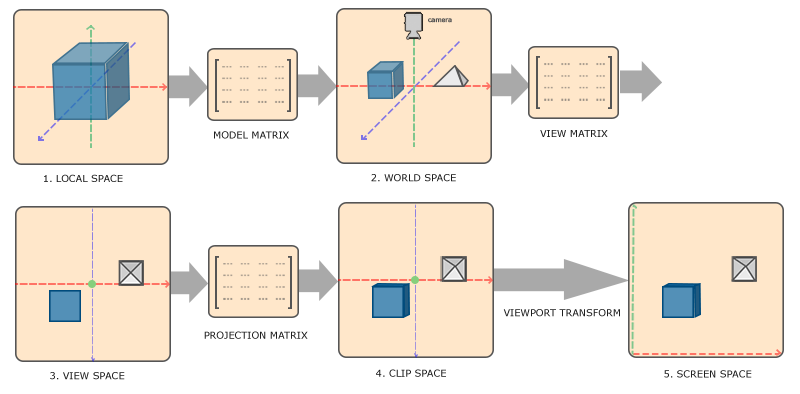
\includegraphics[scale=0.4]{coordinate_systems}



Podemos ver que OpenGL utiliza diferentes sistemas de coordenadas:
\begin{itemize}
	\item \textbf{Coordenadas locales} (local coordinates): coordenadas del objeto relativas a su propio origen.
	\item \textbf{Coordenadas del mundo} (world coordinates): coordenadas del objeto relativas a un origen global del sistema, donde están situados los demás objetos.
	\item \textbf{Coordenadas de vista} (view coordinates): coordenadas del objeto desde el punto de vista de la cámara.
	\item \textbf{Coordenadas de recorte} (clip coordinates): coordenadas respecto a un cubo virtual desde el que determinaremos qué vértices se verán en la pantalla. El cubo tiene dimensiones $[-1,1]\times [-1,1]\times [-1,1]$.
	\item \textbf{Coordenadas de pantalla} (screen coordinates): coordenadas del objeto tal y como lo vemos representado en la pantalla. El origen de las coordenadas de pantalla está situado en la en la esquina inferior izquierda de la pantalla.
\end{itemize} 

Además en la aplicación que vamos a desarrollar queremos que se representen una serie de puntos. Estos puntos estarán situados sobre un nuevo sistema de referencia, con un punto que llamaremos ''de referencia'', situado en el origen, y los demás puntos que llamaremos ''targets'', situados en una circunferencia de radio $2$. Sobre este sistema de referencia realizaremos el análisis de los datos que obtengamos al realizar el experimento, y a estas coordenadas las vamos a llamar coordenadas finales.

\begin{itemize}
	\item \textbf{Coordenadas finales}: sistema de coordenadas que hemos introducido nosotros y que utilizaremos para situar de una forma más cómoda los puntos que representaremos en la aplicación.
\end{itemize}

%https://learnopengl.com/Getting-started/Coordinate-Systems
%https://programmerclick.com/article/7153348621/


Las coordenadas que Touch nos proporciona están en el sistema de referencia local. Por lo tanto nuestro objetivo es estudiar las transformaciones que se realizan para, a partir de esas coordenadas, obtener las coordenadas finales.

Como hemos estudiado en la sección anterior las transformaciones entre sistemas de referencia se realizan a través de la multiplicación de las matrices de cambio de sistema de referencia. Estas matrices en OpenGL tienen los siguientes nombres:

\begin{itemize}
	\item \textbf{Matriz modelo} (model matrix): matriz de cambio del sistema de referencia local al sistema de referencia del mundo.
	\item \textbf{Matriz de vista} (view matrix): matriz de cambio del sistema de referencia del mundo al sistema de referencia de vista.
	\item \textbf{Matriz de proyección} (projection matrix): matriz de cambio del sistema de referencia de vista al sistema de referencia de recorte.
	\item \textbf{Viewport}: matriz de cambio de sistema de referencia de recorte al sistema de referencia de pantalla.
\end{itemize}

 OpenGL combina la matriz modelo y la matriz vista en una matriz llamada \textbf{modelview}. Además, como hemos introducido otro sistema de referencia, tenemos que definir otra matriz para pasar de sistemas de coordenadas de pantalla a sistema de coordenadas finales. Esta matriz la llamaremos la \textbf{matriz final}.

Por tanto el diagrama que vamos a seguir es:

\begin{enumerate}
	\item Aplicamos las transformaciones de OpenGL, es decir:
	\begin{equation}
	C. Locales \rightarrow C. Vista \rightarrow C.Recorte \rightarrow C.Pantalla
	\end{equation}
	\item Aplicamos la matriz final para obtener las coordenadas finales
	\begin{equation}
		C.Pantalla \rightarrow C.Finales
	\end{equation}
\end{enumerate}


Vamos a definir ahora la notación que vamos a utilizar para representar los distintos sistemas de coordenadas:

\begin{itemize}
	\item $R$: sistema de coordenadas locales
	\item $R'$: sistema de coordenadas de vista
	\item $R''$: sistema de coordenadas de recorte
	\item $R'''$: sistema de coordenadas de pantalla
	\item $R^{\romannumeral 4}$: sistema de coordenadas finales
\end{itemize}

Y las correspondientes matrices de cambio de coordenadas son:

\begin{itemize}
	\item $(Id, R', R)$: modelview
	\item $(Id, R'', R')$: proyección
	\item $(Id, R''', R'')$: viewport
	\item $(Id, R^{\romannumeral 4}, R''')$: matriz final
\end{itemize}

En las siguientes secciones vamos a tomar un punto $v$ en el sistema de coordenadas $R$ y vamos a estudiar las transformaciones que OpenGL le aplica para obtener el punto en el sistema de coordenadas $R^{\romannumeral 4}$. Para ello, utilizando la función $glGetDoublev$ de $Gl.h$, obtendremos las matrices que OpenGL aplica en cada paso y las analizaremos utilizando los conceptos que hemos definido previamente.

%glGetDoublev Gl.h.


\subsection{Paso de coordenadas locales a coordenadas de vista}

OpenGL aplica la transformación de coordenadas locales a coordenadas de vista utilizando una única matriz: la matriz modelview. En este paso vamos a tomar $p_R$ y queremos obtener $p_{R'}$ utilizando $(Id, R', R)$, que será la matriz modelview.
La matriz modelview que utiliza la aplicación es:
$$(Id, R', R) = \begin{pmatrix}
	1 & 0 & 0& 0 \\
	0 & 1&0&0 \\
	0&0&1&-6.49 \\
	0&0&0&1
\end{pmatrix}$$
y, utilizando la proposición \ref{cambio} el cambio de sistema de coordenadas será:
$$\begin{pmatrix}
	1 \\
	p_{R'}
\end{pmatrix} = \begin{pmatrix}
	1 & 0 & 0& 0 \\
	0 & 1&0&0 \\
	0&0&1&-6.49 \\
	0&0&0&1
\end{pmatrix}\cdot \begin{pmatrix}
1 \\
p_{R}
\end{pmatrix}$$
Como hemos explicado antes, esto es una notación abreviada de:
\begin{equation}
p_{R'} = 
\begin{pmatrix}
0\\
0\\
-6.49
\end{pmatrix}
+
\begin{pmatrix}
1&0&0 \\
0&1&0\\
0&0&1
\end{pmatrix}
\cdot p_R
\end{equation}
Por tanto lo que estamos haciendo es una transformación afín, en concreto una traslación del origen del sistema de coordenadas en el eje z.

\subsection{Paso de coordenadas de vista a coordenadas de recorte}
Ahora vamos a hacer el cambio de sistemas de coordenadas de vista al sistema de coordenadas de recorte.

El objetivo de este cambio de sistema de coordenadas es transformar la región visible del espacio en un cubo $[-1,1]\times [-1,1]\times [-1,1]$, utilizando una proyección en perspectiva, como podemos ver en la siquiente imagen.
\\

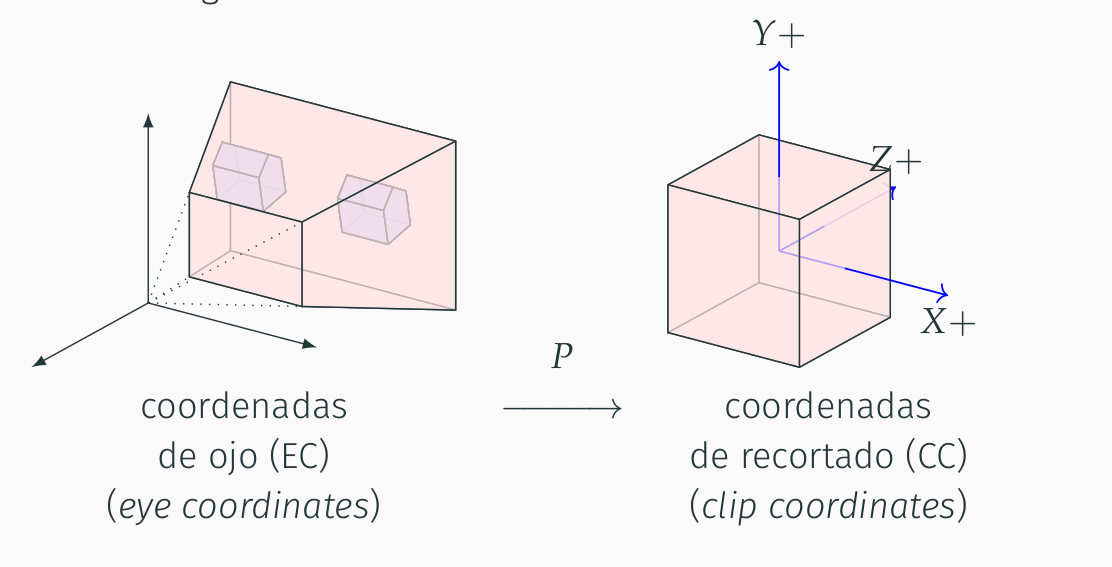
\includegraphics[scale=0.2]{cubo}

La notación que utilizaremos será:
\\

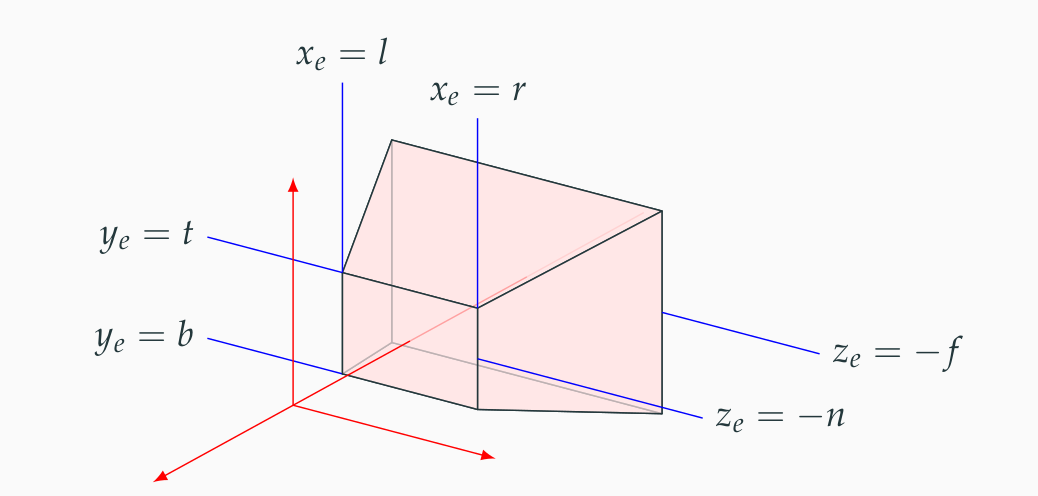
\includegraphics[scale=0.2]{notacion}
\\

Para ello primero calcularemos la proyección en el eje $z$ de las coordenadas $x,y$. Como hemos estudiado antes, para obtener la proyección sobre el plano euclídeo tenemos que dividir por la última coordenada. En este caso como además queremos que los puntos se proyecten sobre el valor $z=-n$, en lugar de $z=1$, tendremos que multiplicar por $-n$. Si tenemos $(x',y',z')$ en el sistema de referencia $R'$.
\begin{equation}
x''_e = x'\cdot\frac{-n}{z'}
\end{equation}
\begin{equation}
y''_e = y'\cdot\frac{-n}{z'}
\end{equation}
\begin{equation}
z''_e = z'\cdot\frac{-n}{z'} = -n
\end{equation}

Tenemos que $(x''_e,y''_e)$ sería el punto que obtendríamos sobre el plano euclídeo (plano situado sobre $z=-n$).

Sabemos ahora que $x''_e \in [l,v]$ y $y''_e \in [b,t]$. Para conseguir que ambos estén en el intervalo $[-1,1]$ tenemos que aplicar un escalado y una traslación. 

\begin{equation}
x'' = 2\cdot(\frac{x''_e-l}{r-l})-1
\end{equation}
\begin{equation}
y'' = 2\cdot(\frac{x''_e-b}{t-b})-1
\end{equation}

Sustituyendo en las ecuaciones anteriores, y utilizando las constantes $a_0,a_1, b_0, b_1$.
\begin{equation}
x'' = \frac{a_0 \cdot x'}{-z'} -a_1 = \frac{a_0 \cdot x'+a_1 \cdot z'}{-z'}
\end{equation}
\begin{equation}
y'' = \frac{b_0 \cdot y'}{-z'} -b_1 = \frac{b_0 \cdot y'+b_1 \cdot z'}{-z'}
\end{equation}
donde
\begin{equation}
a_0 = \frac{2n}{r-l}
\end{equation}
\begin{equation}
a_1 = \frac{r+l}{r-l}
\end{equation}
\begin{equation}
b_0 = \frac{2n}{t-b}
\end{equation}
\begin{equation}
b_1 = \frac{t+b}{t-b}
\end{equation}

Estas transformaciones no se pueden implementar en una matriz, ya que no son lineales (aparece un denominador). Para poder escribirlo en forma de matriz vamos a hacer uso de una coordenada adicional, que nos va a servir para guardar el término no lineal, en este caso $-z$:

\begin{equation}
x'' = a_0 \cdot x'+a_1 \cdot z'
\end{equation}
\begin{equation}
y'' = b_0 \cdot y'+b_1 \cdot z'
\end{equation}
\begin{equation}
w'' = -z'
\end{equation}

La matriz que transforma las coordenadas $(x',y',z')$ en las coordenadas $(x'',y'',w'')$ es:

$$\begin{pmatrix}
x''\\
y''\\
w
\end{pmatrix}=
\begin{pmatrix}
	a_0 & 0&a_1\\
	0&b_0&b_1\\
	0&0&-1
\end{pmatrix}*
\begin{pmatrix}
x'\\
y'\\
z'
\end{pmatrix}
$$


De esta forma, una vez aplicadas las transformaciones afines, podemos obtener las coordenadas del plano de la siguiente forma:
\begin{equation}
(x'',y'',w'') \rightarrow (\frac{x''}{w''}, \frac{y''}{w''})
\end{equation}


Con este procedimiento tendríamos calculadas las coordenadas $x,y$ de pantalla. Sin embargo OpenGL utiliza EPO (eliminación de partes ocultas) para dibujar los objetos en la pantalla, lo que significa que tenemos que guardar información sobre la profundidad, para saber qué puntos están más cerca de otros y así poder superponerlos adecuadamente. 

Para ello vamos a  utilizar una función lineal en la coordenada $z$, que lleve el rango $[-f,-n]$ a $[-1,1]$:

\begin{equation}
z'' = \frac{c_0\cdot z'+c_1}{-z'}
\end{equation}
donde
\begin{equation}
c_0 = \frac{n+f}{n-f}
\end{equation}
\begin{equation}
c_1 = \frac{2fn}{n-f}
\end{equation}

Incluyendo ahora esta nueva ecuación en la matriz anterior tenemos:

$$\begin{pmatrix}
x''\\
y''\\
z'' \\
w
\end{pmatrix}=
\begin{pmatrix}
a_0 & 0&a_1&0\\
0&b_0&b_1&0\\
0&0&c_0&c_1\\
0&0&-1&0
\end{pmatrix}\cdot 
\begin{pmatrix}
x'\\
y'\\
z'\\
1
\end{pmatrix}
$$

Este sería el cambio de sistema de coordenadas que estábamos buscando. Comprobamos ahora que la matriz de proyección que utilizamos en la aplicación tiene esta forma (la obtenemos con \textit{glGetDoublev}):

$$\begin{pmatrix}
2.74748 & 0&0&0\\
0&2.74748 &0&0\\
0&0&-3.74748&-22.5922\\
0&0&-1&0
\end{pmatrix}$$

La matriz tiene la estructura que hemos definido, siendo:
$$a_0 = 2.74748\textup{;  }
a_1 = 0\textup{;  }
b_0 = 2.74748\textup{;  }
b_1 = 0\textup{;  }
c_0 = -3.74748\textup{;  }
c_1 = -22.5922\textup{;  }
$$

\subsection{Paso de coordenadas de recorte a coordenadas de pantalla}
Por lo tanto ya tenemos las coordenadas de recorte y ahora vamos a calcular las coordenadas de pantalla. Las coordenadas de pantalla se expresan en píxeles y nos dicen cuál va a ser la representación del objeto en la pantalla del ordenador.

Los parámetros de la ventana que vamos a utilizar son:
\begin{itemize}
	\item $x_l, y_b$: número de columna y fila que ocupa la esquina inferior izquierda de la ventana.
	\item $w,h$: anchura y altura de la ventana
	\item $n_d, f_d$: rango de valores de z, siendo $n_d$ la profundidad más cercana al observador y $f_d$ la más lejana.
\end{itemize}
Podemos verlo en la siguiente imagen:
\\

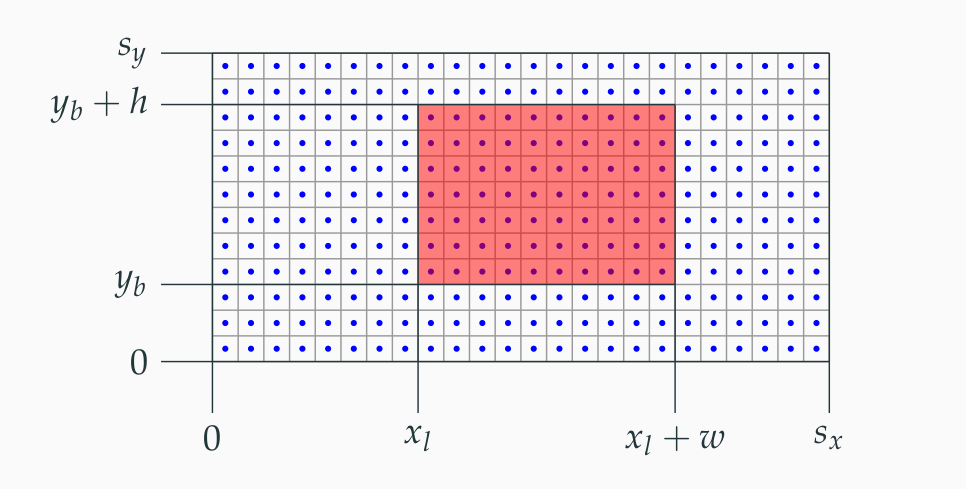
\includegraphics[scale=0.2]{viewport}
\\

Las condiciones que tenemos que realizar para pasar de coordenadas de recorte a coordenadas de pantalla son:
\begin{itemize}
	\item en el eje de coordenadas $x$ tenemos que llevar el intervalo $[-1,1]$ al intervalo $[x_l, x_l+w]$.
	\item en el eje de coordenadas $y$ tenemos que llevar el intervalo $[-1,1]$ al intervalo $[y_b, y_b+h]$.
	\item en el eje de coordenadas $z$ tenemos que llevar el intervalo $[-1,1]$ al intervalo $[n, f]$.
\end{itemize}

Por tanto las transformaciones que tenemos que aplicar son:
\begin{equation}
x''' = (x''+1)\cdot \frac{w}{2}+a
\end{equation}
\begin{equation}
y''' = (y''+1)\cdot \frac{h}{2}+b
\end{equation}
\begin{equation}
z''' = (z''+1)\cdot \frac{f-n}{2}+n
\end{equation}

Las cuales las podemos representar en la matriz:
\begin{equation}
\begin{pmatrix}
x'''\\
y'''\\
z'''\\
1
\end{pmatrix} =
\begin{pmatrix}
\frac{w}{2} &0&0&\frac{w}{2}+a\\
0&\frac{h}{2} &0&\frac{h}{2}+b\\
0&0&\frac{f-n}{2} & \frac{f+n}{2}\\
0&0&0&1
\end{pmatrix}
\cdot \begin{pmatrix}
x''\\
y''\\
z''\\
1
\end{pmatrix}
\end{equation}

En la que podemos ver que estamos aplicando un escalado $[\frac{w}{2}, \frac{h}{2}, \frac{f-n}{2}]$ y una traslación $[\frac{w}{2}+a, \frac{h}{2}+b, \frac{f+n}{2}]$. OpenGL toma $f=1$ y $n=0$ y guarda los valores de $(a,b,w,h)$ en el vector viewport. 

\subsection{Paso de coordenadas de pantalla a coordenadas finales}´

Por último tenemos que pasar de coordenadas de pantalla a las coordenadas  finales que son las que utilizaremos para dibujar las trayectorias.

Para ello vamos a realizar dos transformaciones afines:
\begin{itemize}
	\item Queremos que nuestro ''punto de referencia'' esté en el origen del sistema de coordenadas. Al haber hecho una proyección para pasar de sistemas de coordenadas locales a sistemas de coordenadas de pantalla sabemos que un punto en las coordenadas de pantalla corresponde a una recta en las coordenadas de dispositivo. En concreto el punto de referencia que estamos buscando es la recta que pasa por el punto $(0,0)$ en las coordenadas de dispositivo. Por tanto, utilizando solo un punto de esa recta (el $(0,0)$) podemos saber cómo se representa en la pantalla. Aplicamos las transformaciones que hemos estudiado antes (modelo-vista-proyección-viewport) al punto $(0,0)$ y nos da $(250,250)$. Por lo tanto la traslación que estamos buscando es la que lleva el punto $(250,250)$ al punto $(0,0)$, es decir:
	\begin{equation}
	x^{\romannumeral 4} = x'''-250
	\end{equation}
	\begin{equation}
	y^{\romannumeral 4} = y'''-250
	\end{equation}
	\item Por otro lado queremos que en nuestro sistema de referencia los ''targets'' estén situados en la circunferencia de radio 2, por lo tanto tenemos que aplicar un escalado. Para saber el escalado que tenemos que hacer aplicamos la transformación modelo-vista-proyección-viewport al ''target'' que en el sistema de referencia final está situado en  $(2\cdot \cos\frac{\pi}{4},2\cdot \sin\frac{\pi}{4})$. Después calculamos la distancia del punto que nos ha dado al punto origen, y dividimos la distancia de nuestro punto origen a nuestro punto objetivo entre esa distancia. El resultado es $0.00945962$, que será el factor de escala.
\end{itemize}
Por último vamos a representar estas transformaciones afines en forma de matriz:

\begin{equation}
\begin{pmatrix}
x^{\romannumeral 4}\\
y^{\romannumeral 4}\\
1
\end{pmatrix} =
\begin{pmatrix}
0.0009 &0&-250\\
0&0.0009&-250\\
0&0&1 \\
\end{pmatrix}
*\begin{pmatrix}
x'''\\
y'''\\
1
\end{pmatrix}
\end{equation}

Y de esta forma ya tenemos todas las transformaciones que vamos a hacer para obtener las coordenadas con las que haremos el análisis de los datos obtenidos.


\chapter{Desarrollo del proyecto}




En este capítulo vamos a hablar de cómo se han desarrollado las diferentes fases del proyecto así como de los resultados obtenidos.

\section{Planificación del experimento}

En esta fase del proyecto decidimos cuál iba a ser la forma que iba a tener el experimento que posteriormente íbamos a realizar.

Desde el primer momento sabíamos que el objetivo era tener una aplicación en la que aparecieran una serie de puntos en la pantalla, y en la que el usuario tuviera que mover el cursor de un punto a otro haciendo movimientos balísticos. Posteriormente queríamos ser capaces de guardar la trayectoria de los movimientos realizados para poder analizarlas después.



\subsection{Diseño de nuestro experimento}

Dado que el objetivo del proyecto era probar el funcionamiento de System3D Touch en este tipo de experimentos, y no disponiendo de otros dispositivos complementarios, decidimos que el experimento consistiera en la aparición en pantalla de una serie de puntos sobre los que el sujeto debería situar el cursor.

Primero tendemos un punto de referencia en el centro, y cuando el sujeto se haya posado sobre él, desaparece este y aparece otro sobre una circunferencia alrededor del punto de referencia, en una de las siguientes posiciones:
\\

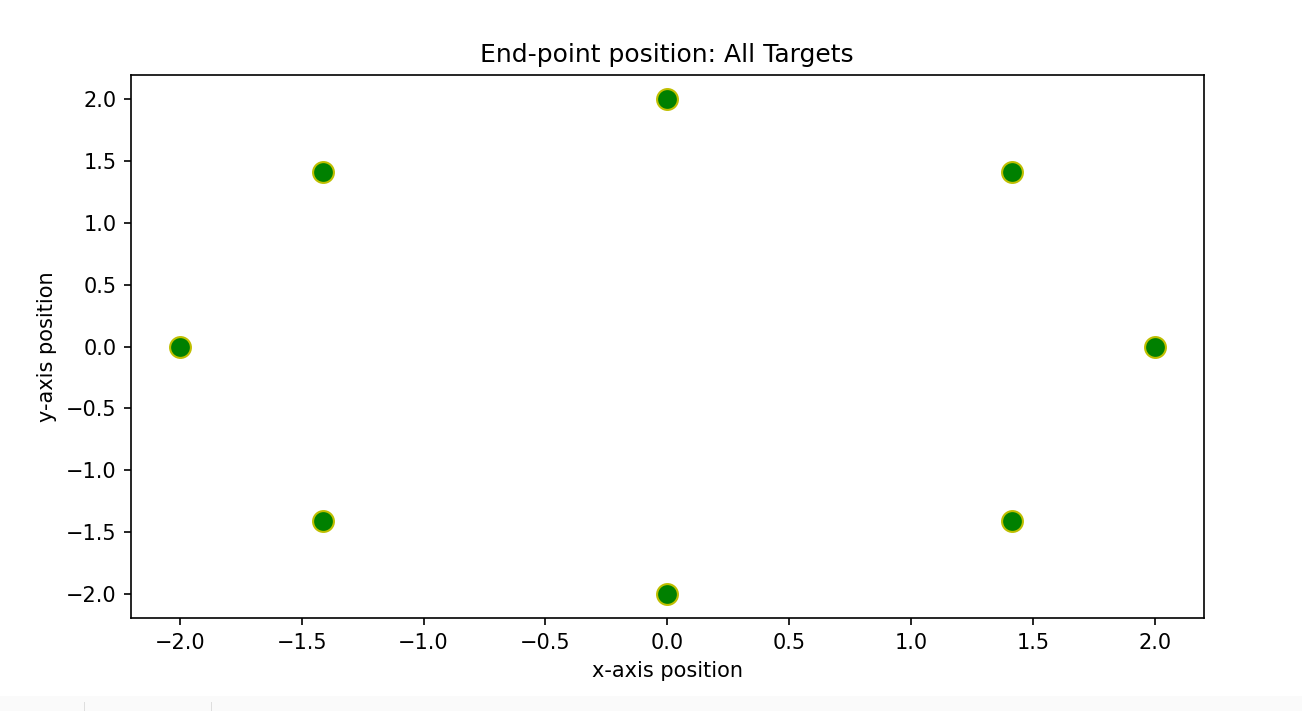
\includegraphics[scale=0.2]{points}
\\


 Al haber situado el cursor sobre el punto objetivo, o al haber terminado el tiempo límite para realizar el movimiento, el punto objetivo desaparece y aparece otra vez el punto de referencia, volviendo a empezar otra iteración. Las trayectorias que nos interesan son las del punto de referencia al punto objetivo.

Tenemos además cinco fases, en las que cambian las condiciones en como se comporta 3DSystem Touch:

\begin{itemize}
	\item \textbf{Fase de adaptación}: en esta fase solo se muestra el cursor sin ningún punto objetivo. El sujeto es libre para hacer cualquier tipo de movimiento. Esta fase sirve para que el sujeto se adapte a la utilización del dispositivo, así como para que tenga en cuenta las condiciones en las que el dispositivo no funciona correctamente, como cuando se acerca o se aleja demasiado en el eje $z$.
	\item \textbf{Fase inicial}, sin ninguna fuerza y mostrando el cursor.
	\item \textbf{Segunda fase}, en la que se muestra el cursor y se aplica una fuerza constante en la dirección x, en sentido negativo.
	\item \textbf{Tercera fase}, en la que no se aplica ninguna fuerza y se oculta el cursor en los movimientos desde el punto de referencia al punto objetivo. Al terminar el movimiento se vuelve a mostrar el cursor para volver al punto de referencia.
	\item \textbf{Cuarta fase}, en la que se aplica la misma fuerza de la segunda fase y se oculta el cursor siguiendo lo explicado en la tercera fase.
\end{itemize}

Los parámetros que tuvimos que elegir para desarrollar la aplicación fueron:
\begin{itemize}
	\item \textbf{Número de repeticiones por fase}. Dado que la realización del experimento requiere de movimientos del brazo durante un periodo de tiempo moderado, teníamos que encontrar un acuerdo entre tener un número suficiente de repeticiones por punto objetivo y que el experimento no fuese demasiado exigente para los individuos. Es por eso por lo que en la fase de prueba probamos diferentes configuraciones con sujetos de diferentes edades, desde 20 a 90 años. Finalmente elegimos tener 80 repeticiones por fase, para así tener 10 repeticiones por punto. Habría que tener en cuenta que en el caso de finalmente realizar el experimento con personas mayores de 80 años, sería recomendable bajar el número de repeticiones.
	\item \textbf{Tiempo para la realización del movimiento}. Este es un parámetro clave a la hora de diseñar el experimento, pues queríamos que los sujetos estuviesen obligados a hacer movimientos balísticos. Por lo tanto teníamos que encontrar un balance entre tener tiempo suficiente para que pudiesen alcanzar el punto y la obligación de que esos movimientos fuesen rápidos. Aquí también encontramos grandes diferencias en los resultados de personas jóvenes y más mayores, pero finalmente decidimos utilizar un tiempo de 2 segundos, con el que, una vez pasado un periodo de aprendizaje, todos los sujetos fueron capaces de alcanzar en ese tiempo el punto objetivo.
	\item \textbf{Número y disposición de los puntos objetivos}. Hicimos pruebas con diferentes sujetos con 8 puntos (como hemos mencionado arriba), 4 puntos en las siguientes posiciones:
	
	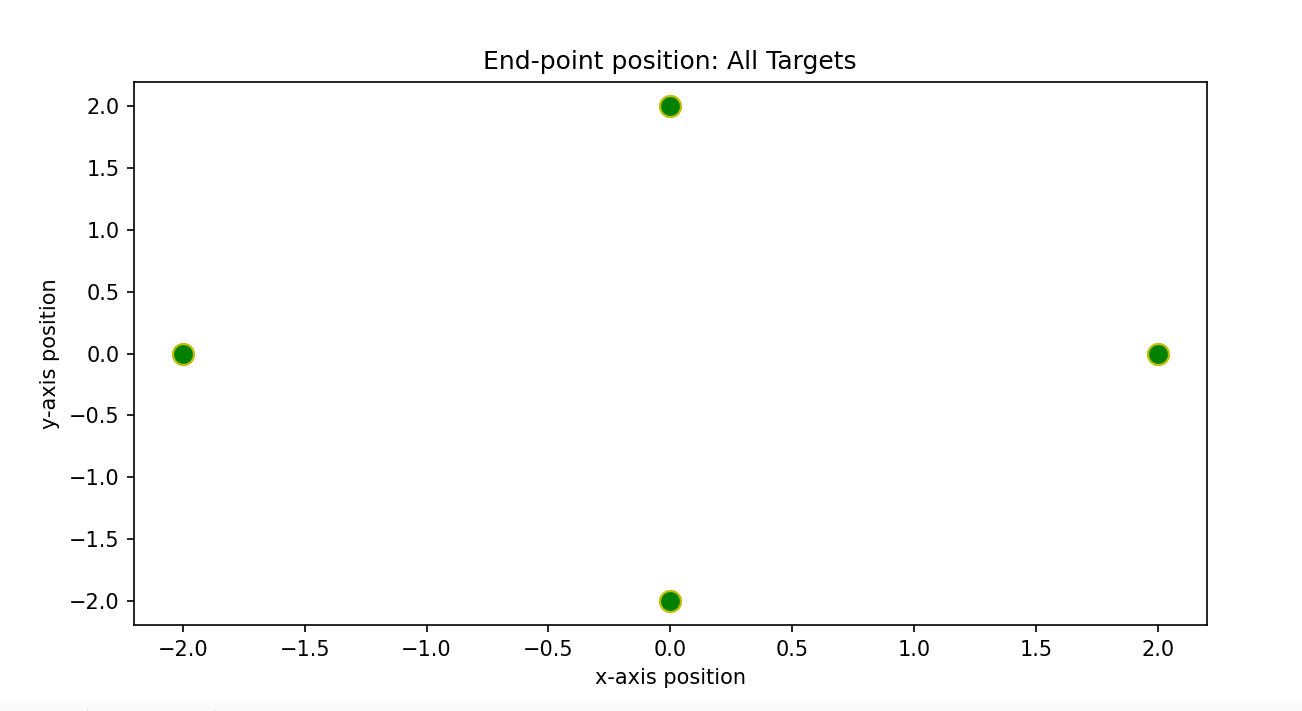
\includegraphics[scale=0.2]{points-4}
	
	 y 2 puntos:
	 
	 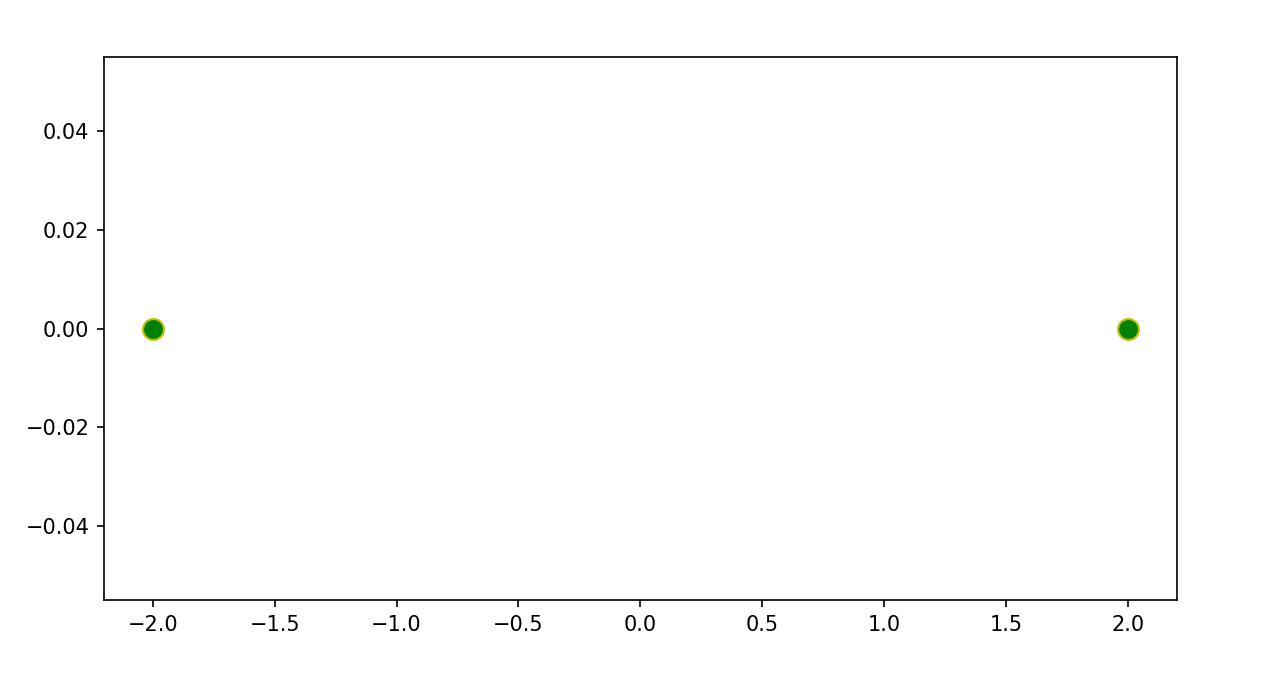
\includegraphics[scale=0.2]{puntos2}
	 
	  Pensamos que el experimento más interesante era con 8 puntos, pues así podíamos estudiar las diferencias en el aprendizaje de movimientos cuando hay que mover el cursor en un solo eje a cuando hay que moverlo en dos ejes a la vez. En todo caso, y en relación con la dificultad en realizar un número grande de iteraciones en personas mayores, podría estudiarse el caso de reducir el número de puntos para así poder reducir a su vez el número de iteraciones.
	\item Disposición de los \textbf{puntos objetivos siguiendo un orden o de forma aleatoria}.
\end{itemize}

Otra decisión que tomamos fue la del criterio para considerar que un movimiento es correcto. En primer lugar pensamos que el criterio fuera que el sujeto pasase el cursor por encima del punto objetivo, de forma similar a como hacen en \textit{''Cerebellar Contributions to Reach Adaptation and Learning Sensory Consequences of Action''}. Después pensamos que sería interesante estudiar también, no solo que los sujetos realizaran el movimiento en la dirección correcta, sino con la distancia correcta. Por eso, para que el movimiento se considere correcto, el sujeto debe situar durante un momento el cursor encima del punto. Hicimos lo mismo a la hora de situar el cursor dentro del punto de referencia, e iniciar así el movimiento. Esto fue debido a que, en una pequeña demo inicial vimos que, si lo hacíamos solo con pasar el cursor sobre el punto de referencia, todos los movimientos empezaban con un desplazamiento en sentido contrario, el correspondiente al movimiento de volver al punto de referencia. De esta forma el sujeto está obligado a pararse dentro del punto inicial e iniciar el movimiento desde ahí.

También introdujimos un sonido cuando el movimiento no se ha realizado de forma correcta. Esto sirve de feedback al usuario, para saber cuando el movimiento se ha realizado correctamente y cuando no. 


\section{Desarrollo de la aplicación}

El objetivo de esta fase es desarrollar una aplicación sobre la que llevar a cabo el experimento diseñado en la fase de planificación, y también una forma de analizar los resultados que tengamos al realizar el experimento. Es decir, queremos tener como resultado:
\begin{itemize}
	\item Una aplicación diseñada para ejecutarse desde el ordenador, pues necesitamos utilizar a su vez el dispositivo Touch. \\
	Dicha aplicación debe tener:
	\begin{itemize}
		\item Un menú de selección para poder elegir entre los 5 modos de uso: libre, sin fuerza, con fuerza, sin fuerza y sin cursor y con fuerza y sin cursor.
		\item Al elegir el modo (salvo eligiendo el modo libre) debe aparecer una tarea que tendrá que realizarse un número determinado de iteraciones y que consistirá en:
		\begin{enumerate}
			\item Aparece el target de referencia, en la posición 0 (el centro).
			\item Al parar el cursor sobre el target de referencia este desaparece y aparece en su lugar un target situado sobre la circunferencia de radio 2 y centro el target de referencia. El nuevo target puede aparecer en cualquiera de las 8 posiciones mencionadas antes.
			\item Al parar el cursor sobre el target objetivo este desaparece y vuelve a aparecer el target de referencia.
		\end{enumerate}
		\item Se deben poder guardar las trayectorias y los tiempos del movimiento desde el target de referencia al target objetivo. Cada una de las 4 fases se guardaŕa en un fichero csv diferente.
	\end{itemize}
	\item Un script de python que lea los ficheros csv generados al realizar el experimento y genere gráficas con los resultados en cada una de las fases de:
	\begin{itemize}
		\item Errores (distancia al target objetivo) en cada iteración. Por un lado queremos tener una gráfica con todos los errores de la fase, y por otro separados según el target objetivo.
		\item Tiempo transcurrido al realizar el movimiento. Al igual que con los errores, por fase y por target objetivo dentro de la fase.
		\item Distancia y velocidad al punto objetivo a través del tiempo, en cada uno de los ejes. Separado por targets objetivos.
	\end{itemize}
\end{itemize}


La fase del desarrollo de la aplicación tuvo tres partes: instalación del software necesario, implementación del código y revisión del código una vez elegidos los parámetros.

\subsection{Instalación del software de OpenHaptics}

La primera decisión que tuvimos que tomar fue si instalar el software de OpenHaptics en una máquina Ubuntu, o en una máquina Windows. Aunque en un principio la opción inicial fue instalarlo en Ubuntu 20.04, después de una prueba nos dimos cuenta de que Windows soportaba mejor la interfaz gráfica necesaria para llevarlo a cabo. Por tanto procedimos a realizar la instalación en Windows.

Los paquetes utilizados pueden encontrarse \href{https://support.3dsystems.com/s/article/OpenHaptics-for-Windows-Developer-Edition-v35?language=en\_US}{aquí}. Tenemos que instalar las \href{https://s3.amazonaws.com/dl.3dsystems.com/binaries/Sensable/OH/3.5/OpenHaptics_Developer_Edition_v3.5.0.zip}{librerías de OpenHaptics} y los \href{https://s3.amazonaws.com/dl.3dsystems.com/binaries/Sensable/driver/Touch_Device_Driver_2023.1.4.exe}{drivers de Touch}.
El toolkit de OpenHaptics necesita ciertos requerimientos hardware:
\begin{itemize}
	\item Procesador : 
	\begin{itemize}
		\item Intel i5 / i7, 5ª Generación o mayor 
		\item CPU mínimo 2.5 GHz de frecuencia.
		\item RAM 4 GB.
	\end{itemize}
	\item Tarjeta gráfica de mínimo 256 MB VRAM .
	\item Espacio de disco 512 MB.
	\item Resolución de pantalla 1280 x 800 (mínimo).
\end{itemize}
y software:
\begin{itemize}
	\item Sistema Operativo 64-bit Windows 7, 8.1, y 10
\end{itemize}

Tenemos tres documentos que nos servirán de ayuda para instalar y desarrollar utilizando OpenHaptics:
\begin{itemize}
	\item \textbf{OpenHaptics Installation Guide}: guía de instalación del toolkit de OpenHaptics.
	\item \textbf{Programmer’s Guide}: guía que explica la arquitectura de OpenHaptics, cómo funciona y lo que se puede hacer. Hay ejemplos de código, una explicación de cómo configurar Visual Studio para trabajar con la librería y una visión general de las tres APIs: QuickHaptics, HLAPI y HDAPI.
	\item \textbf{API Reference Guide}: contiene documentación sobre las funciones de QuickHaptics, HLAPI y HDAPI.
\end{itemize}

Las librerías de OpenHaptics están en c++, por lo tanto será el lenguaje de programación que utilizaremos. Las tres APIs que incluye son, como hemos comentado antes:
\begin{itemize}
	\item \textbf{QuickHaptics}: permite escribir rápido y fácilmente nuevas aplicaciones hápticas, o añadir funcionalidades hápticas a aplicaciones ya existentes.  
	\item \textbf{HDAPI}: provee un acceso a bajo nivel al dispositivo háptico, lo que permite a los programadores controlar las fuerzas que se pueden aplicar. 
	\item \textbf{HLAPI}: provee un acceso a alto nivel, similar a la API de OpenGL. Permite la reutilización de código de OpenGL.
\end{itemize}
En la siguiente imagen podemos ver cómo se relacionan las tres APIs:
\\
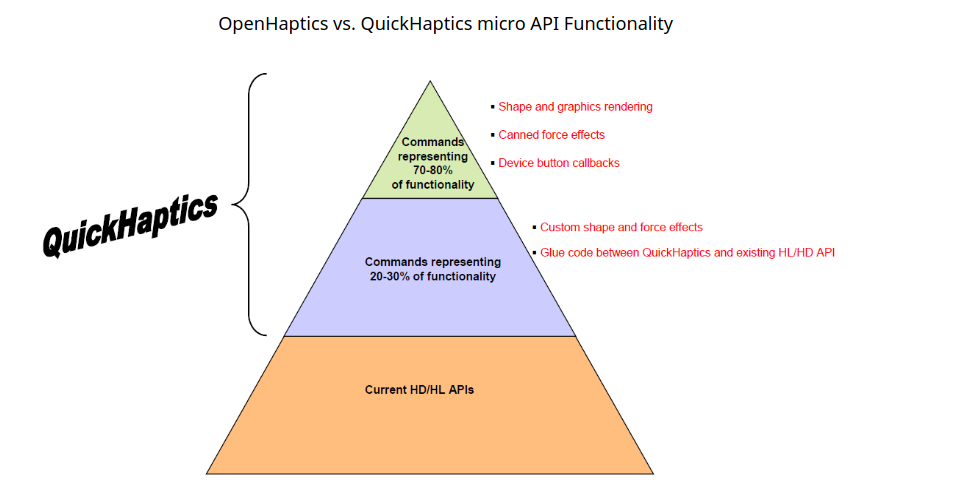
\includegraphics[scale=0.4]{OPENHAPTICS}
\\

En nuestro caso utilizaremos HDAPI, pues necesitamos controlar la fuerza que le aplicamos al dispositivo. También utilizaremos la biblioteca GLUT, una biblioteca de utilidades de OpenGL que nos permite manejar ventanas y representaciones gráficas.

\subsection{Implementación del codigo}

La estructura de un programa que utilice OpenHaptics es la siguiente: 


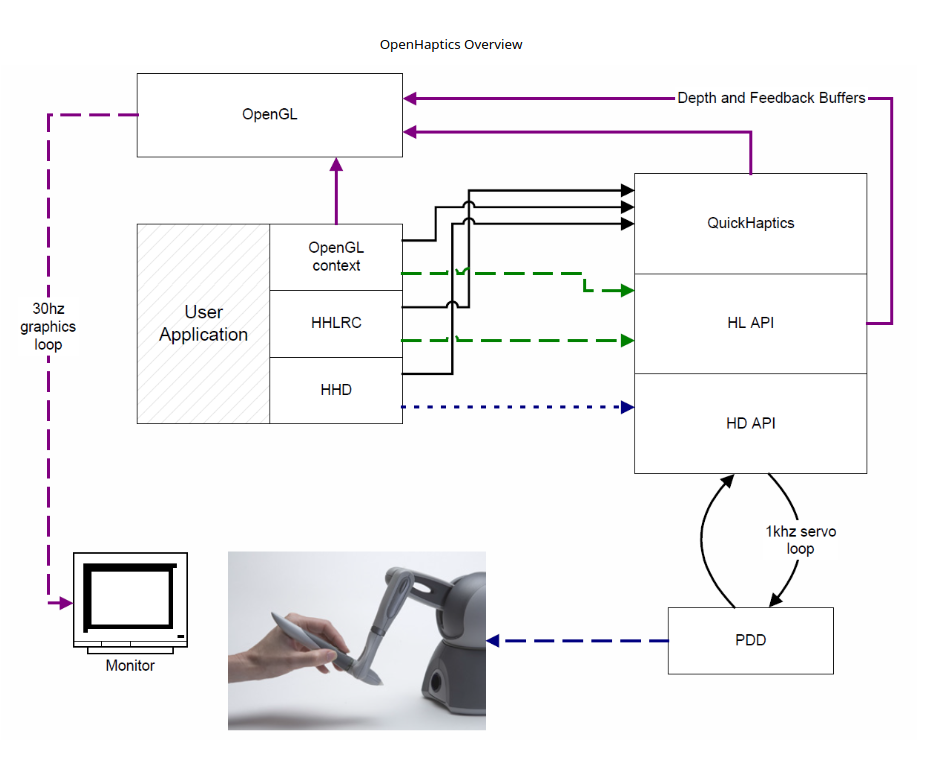
\includegraphics[scale=0.4]{estructura}

Como podemos ver tenemos dos bucles: el \textbf{bucle gráfico} y el \textbf{servoloop}.

El servo loop se usa para controlar las fuerzas que se mandan al dispositivo háptico. Para mantener un feedback consistente este bucle debe ejecutarse al menos a una frecuencia de 1000Hz, por lo que se ejecuta en una hebra diferente, con prioridad máxima. Para inicializar el servoloop utilizamos la función de HDAPI \textit{hdStartScheduler()}. Se debe llamar una vez que se han inicializado las rutinas del dispositivo y se han añadido las callbacks asíncronas del scheduler. Una vez inicializado el servoloop empiezan a ejecutarse las callbacks que hemos definido, en cada iteración del bucle.

El bucle gráfico se ejecuta en una hebra diferente, y dado que el ojo humano no es capaz de procesar tantas imágenes por segundo, la frecuencia del bucle será menor, en concreto de 30Hz. El bucle gráfico se encarga de actualizar la representación gráfica, según los eventos que ocurran. Para inicializar el bucle gráfico utilizamos la función de GLUT \textit{glutMainLoop()}. Una vez inicializado el bucle gráfico se llamarán en cada iteración a las callbacks que hayamos definido.

Dado que la frecuencia a la que se ejecutan los dos bucles es diferente, podemos tener problemas a la hora de que la hebra gráfica pida información a la hebra háptica sobre el estado del dispositivo. Para que el estado del dispositivo sea consistente se utiliza el scheduler, que provee sincronización entre las dos hebras.

Las callbacks del servoloop pueden ser \textbf{síncronas} o \textbf{asíncronas}. Las callbacks síncronas se usan principalmente para tener una instantánea del estado del dispositivo. Las callbacks síncronas solo devuelven el control de la hebra una vez terminadas, por lo que la aplicación tiene que esperar a que la función se haya terminado. Las callbacks asíncronas, por el contrario, devuelven el control justo cuando son programadas, por lo que la aplicación puede seguir ejecutándose. Son adecuadas para representar un efecto háptico, pues pueden perdurar en el tiempo, ya que en cada iteración se aplicará el efecto de la callback al dispositivo.

Las callbacks pueden devolver dos tipos de valores: \textit{DONE} y \textit{CONTINUE}. Las callbacks con return code \textit{DONE} no volverán a ser ejecutadas en el bucle del servoloop hasta que vuelvan a ser programadas. Por el contrario, las callbacks con return code \textit{CONTINUE} se vuelven a programar para la próxima iteración del bucle, hasta que explícitamente se especifique que se desprograme.

En nuestro caso las callbacks del servoloop son:
\begin{itemize}
	\item \textit{beginUpdateCallback}: callback asíncrona, con return code \textit{CONTINUE}. Se programa al inicializar el dispositivo háptivo y es la callback principal de la hebra háptica.  Actualiza el estado del dispositivo háptivo y escribe en el fichero csv las coordenadas del dispositivo (en caso de que se haya empezado el movimiento de ir desde el target de referencia al target objetivo, a lo que nos referiremos con que se ha inicializado la acción). 
	
	Dependiendo del momento de:
	\begin{itemize}
		\item Si la acción se ha inicializado comprueba el tiempo que ha transcurrido desde que se empezó la acción: si ha superado el tiempo límite programa la callback \textit{actionFinished}.
		\item Si el cursor está en contacto con el punto de referencia, no se ha inicializado la acción y no estamos en la fase libre del experimento: comprueba si el cursor ha estado parado el tiempo necesario sobre el punto de referencia, si es así programa la callback \textit{actionInitialized}.
		\item Si el cursor está en contacto con el target objetivo en esa iteración, la acción se ha inicializado y no estamos en la fase libre del experimento: si el cursor ha estado parado el tiempo necesario sobre el target objetivo se programa la callback \textit{actionFinished}.
	\end{itemize}
	
	\item \textit{setDeviceTransformationCallback}: callback síncrona, con return code \textit{DONE}. Se programa al actualizar las transformaciones de coordenadas y calcula las transformaciones que hay que realizar.
	
	\item \textit{forceCallback}: callback asíncrona, con return code \textit{CONTINUE}. Se programa en la callback \textit{actionInitialized} y aplica la fuerza que hemos configurado al dispositivo. 
	
	\item \textit{clearForceCallback}: callback asíncrona, con return code \textit{CONTINUE}. Se programa en la callback \textit{actionFinished} y elimina la fuerza que se había aplicado antes, poniendo el vector fuerza nuevamente a 0. 
	
	\item \textit{actionInitialized}: callback asíncrona, con return code DONE. Se programa en la callback \textit{beginUpdateCallback} y sus funciones son:
	\begin{itemize}
		\item Oculta el target de referencia.
		\item Calcula el siguiente target objetivo y lo hace visible.
		\item Si estamos en algunas de las fases en las que se aplica fuerza al dispositivo, programa la callback forceCallback. 
		\item Inicializa el tiempo de inicio de acción.
		\item Si estamos en alguna de las fases en las que se oculta el cursor, hace el cursor no visible.
	\end{itemize}
	
	\item \textit{actionFinished}: callback asíncrona con return code DONE. Se programa en la callback \textit{beginUpdateCallback} y sus funciones son:
	\begin{itemize}
		\item Oculta el target objetivo.
		\item Muestra el target de referencia.
		\item Programa la callback \textit{clearForceCallback}.
		\item Muestra el cursor.
		\item Si se han terminado las iteraciones diseñadas para la fase, selecciona la fase libre del experimento.
	\end{itemize}
\end{itemize}
Y las del bucle gráfico:
\begin{itemize}
	\item \textit{glutDisplayFunc}: callback que se utiliza para actualizar la vista. En esta callback actualizamos el estado del dispositivo, capturando el último estado del servoloop. También dibujamos la escena, según el modo del menú que se haya elegido. 
	
	\item \textit{glutReshapeFunc}: callback para actualizar las dimensiones de la ventana. También se actualiza la posición de la cámara.
	
	\item \textit{glutIdleFunc}: callback para mandar una petición de redibujar la ventana.	
\end{itemize}

Vamos a hablar ahora del main y de las dos clases más importantes de la aplicación: HapticDeviceManager y PointManager.

\subsubsection{Main}

Las funciones del main son:
\begin{itemize}
	\item Inicializar la librería de GLUT: lo hacemos con la función \textit{glutInit()}.
	\item Crear y definir las dimensiones de la pantalla y el modo de visualización: \textit{glutCreateWindow()}, \textit{glutInitDisplayMode()} y \textit{glutInitWindowSize()}.
	\item Definir las callbacks que actualizarán el entorno gráfico: \textit{glutDisplayFunc}, \textit{glutReshapeFunc} y \textit{glutIdleFunc}. 
	\item Crear el menú: \textit{glutAttachMenu()} y \textit{glutAddMenuEntry()}.
	\item Inicializar la escena que vamos a representar: inicializamos OpenGL, creamos un objeto de la clase PointManager y otro objeto de la clase HapticDeviceManager, al que le pasamos el objeto PointManager como parámetro.
	\item Inicializar el bucle gráfico: \textit{glutMainLoop()}.
\end{itemize}




\subsubsection{Clase HapticDeviceManager}

Esta clase nos permite integrar las interacciones hápticas con la lógica y el estado de la aplicación.

Las funciones son llamadas desde el objeto HapticDeviceManager que hemos creado en el main. Las más importantes son:

\begin{itemize}
	\item \textit{setUp}: inicializamos el dispositivo háptico. y programamos la callback \textit{beginUpdateCallback}. Inicializamos el scheduler para que empiece el bucle del servoloop. También inicializamos el atributo PointManager con el parámetro que hemos pasado a la función.

	
	\item \textit{updateState}: se llama en cada iteración del ciclo gráfico. Sincroniza el estado con el thread háptico.
	
	\item \textit{updateWorkspace}: calcula las transformaciones necesarias para pasar de coordenadas del dispositivo a coordenadas del mundo. También programa la callback \textit{setDeviceTransformCallback}.
		
	\item \textit{drawCursor}: utiliza las funciones de OpenGL para dibujar el cursor en la pantalla.
	
	\item \textit{setManipulationStyle}: configura la fase del experimento (libre, sin fuerza, con fuerza, sin fuerza sin cursor, con fuerza sin cursor) según la opción seleccionada en el menú.
\end{itemize}


\subsubsection{Clase PointManager}

Esta clase nos permite manejar los puntos que aparecen en la escena, desde el números de puntos que hay, dónde están situados y las características que tienen. Cada punto tendrá un estado asociado: HighLighted y Selected. El punto tendrá estado HighLighted cuando aparezca en pantalla, y Selected cuando esté oculto. Las funciones más importantes de la clase son:

\begin{itemize}
	\item \textit{setUp}: aquí definimos el número de puntos que hay en la escena, dónde están situados y su estado. En nuestro caso definimos 9 puntos: el punto de referencia con estado HighLighted, y los demás, es decir, los puntos targets, con estado Selected.
	
	\item \textit{updatePointSize}: Determina el factor de escala para transformar las coordenadas a coordenadas de pantalla y dibujar los puntos en dimensiones de píxeles.
	
	\item \textit{drawPoints}: Dibuja los puntos, dependiendo del estado que tengan y teniendo en cuenta el factor de escala calculado en \textit{updatePointSize}.
	
	\item \textit{getPointPosition/setPointPosition}: devuelve o configura la posición de punto según el índice pasado, en coordenadas del mundo.
	
	\item \textit{setPointHighlighted/Selected}: cambia el estado del punto a HighLighted o Selected, según la función.
	
	\item \textit{isPointHighlighted/Selected}: devuelve un boolean indicando si el punto tiene estado HighLighted o Selected.
	
	\item \textit{getNumPoints}: devuelve el número de puntos que hemos configurado. Los puntos se guardan en un array.
\end{itemize}

En la siguiente imagen podemos ver representada la estructura que hemos explicado.

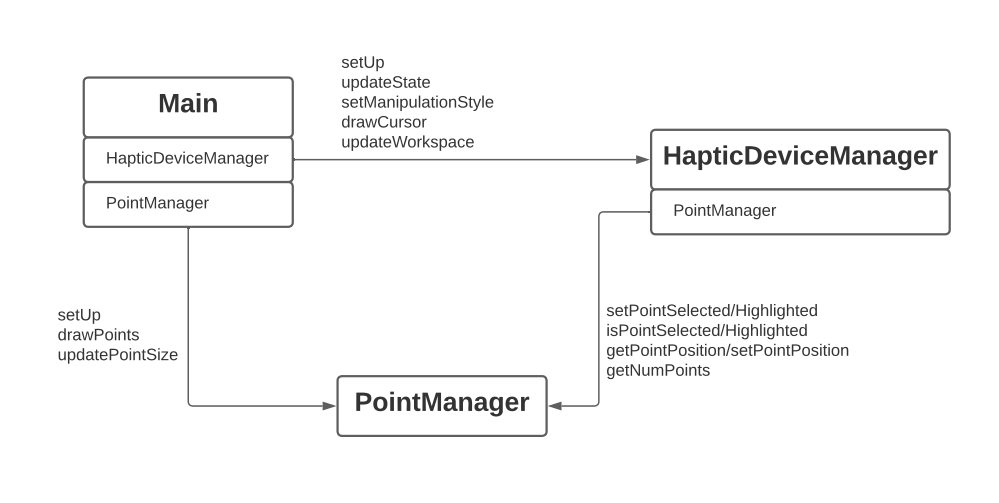
\includegraphics[scale=0.4]{diagrama}

\subsubsection{Guardado de datos}

Para guardar los datos obtenidos de las trayectorias punto\_inicial-punto\_objetivo utilizamos excel. Guardamos los datos en cuatro ficheros diferentes, uno por cada fase del experimento. Cada fichero contiene cinco columnas:
\begin{itemize}
	\item Coordenada x del cursor
	\item Coordenada y del cursor
	\item Número de iteración. Una iteración es un movimiento desde el punto inicial al objetivo.
	\item Punto objetivo. Numerados del 1 al 8.
	\item Tiempo transcurrido desde que se empieza el movimiento, en nanosegundos.
\end{itemize}

Al terminar el experimento analizaremos las gráficas obtenidas con un script de python.

\subsection{Script de python}

El script de python toma los datos de los ficheros excel generados en el desarrollo de experimento, utilizando el módulo pandas.

Después, para cada individuo y cada fase representa las siguientes gráficas:

\begin{itemize}
	\item Gráfica con las trayectorias de todas las iteraciones. A medida que se realizan más trayectorias en un target determinado las líneas son más oscuras. También se representan los targets finales.
	\item Gráfica con los puntos finales de los movimientos. A medida que se realizan más trayectorias en un target determinado las líneas son más oscuras. También se representan los targets finales.
	\item Gráfica con la evolución de los errores respecto al número de iteraciones realizado, agrupados por target. Cada target tiene asociado un color.
	\item Gráfica con la evolución del tiempo necesario para realizar el movimiento respecto al número de iteraciones realizado, agrupados por target. Cada target tiene asociado un color.
\end{itemize}

La distancia que utilizamos para calcular los errores es la distancia euclidea.

\section{Obtención de resultados}

Como hemos mencionado en la sección Fases del proyecto, llevamos a cabo dos tandas de experimentos: una primera fase de prueba, para decidir los parámetros que íbamos a utilizar; y una segunda fase final para poder obtener resultados.

Uno de los requisitos era que en cada una de las fases tuviésemos representación de individuos de distintas edades, para no tener un sesgo a la hora de implementarla y obtener resultados válidos. Teniendo en cuenta esto, y la disponibilidad de personas que teníamos a nuestro alrededor, los sujetos elegidos para cada una de las fases fueron:
\\


\begin{tabular}{l l | l l}
	\multicolumn{2}{ c }{Fase 1} & \multicolumn{2}{ c }{Fase 2} \\ 
	Sexo & Edad & Sexo & Edad\\\hline 
	
	Mujer & 23 & Mujer & 20 \\
	Mujer & 24  & Mujer & 22\\
	Hombre & 53 & Hombre & 50\\
	Mujer & 52 & Hombre & 60 \\
	Hombre & 62  & Mujer & 59\\\
	Mujer & 60 \\
	Hombre & 90 \\
	Mujer & 90 \\
\end{tabular} 
\\

Como se puede comprobar, en la segunda fase la muestra de individuos fue similar a la primera, salvo porque no tuvimos individuos mayores de 80 años. Esto fue debido en parte a la poca disponibilidad que teníamos de individuos de edad más avanzada, y en parte a que decidimos realizar el experimento en unas condiciones que les eran menos favorables, con demasiadas repeticiones. Ninguno de los sujetos del experimento tenían un problema cerebral reconocido, por lo que podemos suponer que eran individuos sanos. No pudimos probar el experimento en individuos con problemas en el cerebelo, como hubiese sido lo ideal, por falta de disponibilidad.


En la segunda fase, para poder obtener algunas conclusiones de cómo afecta el orden de aparición de targets en la realización de los movimientos (si aparecen los targets en orden, o de forma aleatoria) a algunos de los individuos le aparecieron los puntos en orden y a otros no. A continuación aparecen los sujetos de la segunda fase con sus respectivas características y el modo de experimento que hicieron (en orden o aleatorio). Esta será la nomenclatura que utilizaremos a partir de ahora.

\begin{itemize}
	\item Sujeto 1: Mujer, 20 años, en orden
	\item Sujeto 2: Mujer, 22 años, aleatorio
	\item Sujeto 3: Mujer, 60 años, aleatorio
	\item Sujeto 4: Hombre, 50 años, en orden
	\item Sujeto 5: Hombre, 60 años, en orden
\end{itemize}

Todos los sujetos realizaron las fases del experimento en orden y tuvieron 2 minutos de descanso entre fase.

% Foto aplicación
% Foto gente haciendo el experimento

Además todos los individuos firmaron una declaración de ...

\section{Analisis de resultados}


%For analysis of hand trajectories, we used Savitzky–Golay
%smoothing filter for the measured hand position and velocity.
En esta sección analizaremos los resultados que obtuvieron cada uno de los cinco sujetos. Para ello lo dividiremos en dos secciones: primero compararemos cuáles fueron las diferencias entre los diferentes individuos en cada una de las fases, y luego estudiaremos las diferencias entre los resultados de cada fase de cada uno de los individuos.


\subsection{Análisis de la misma fase entre individuos}

En este análisis queremos estudiar cuál ha sido el rendimiento de cada sujeto, comparado con el rendimiento de los demás. De esta forma queremos poder tener datos para estudiar cómo influyen factores como la edad y la aparición en orden o no de los puntos.

\subsubsection{Sin fuerza}
Podemos observar una diferencia entre los sujetos de mayor edad y los más jóvenes. Mientras que en los sujetos más jóvenes los puntos se concentran alrededor de los puntos objetivos (hay una gran precisión), en los de mayor edad están más dispersos:

Sujetos menores de 60 años:
\\
\begin{figure}[h]
	\begin{minipage}[b]{0.5\linewidth}
		\centering
		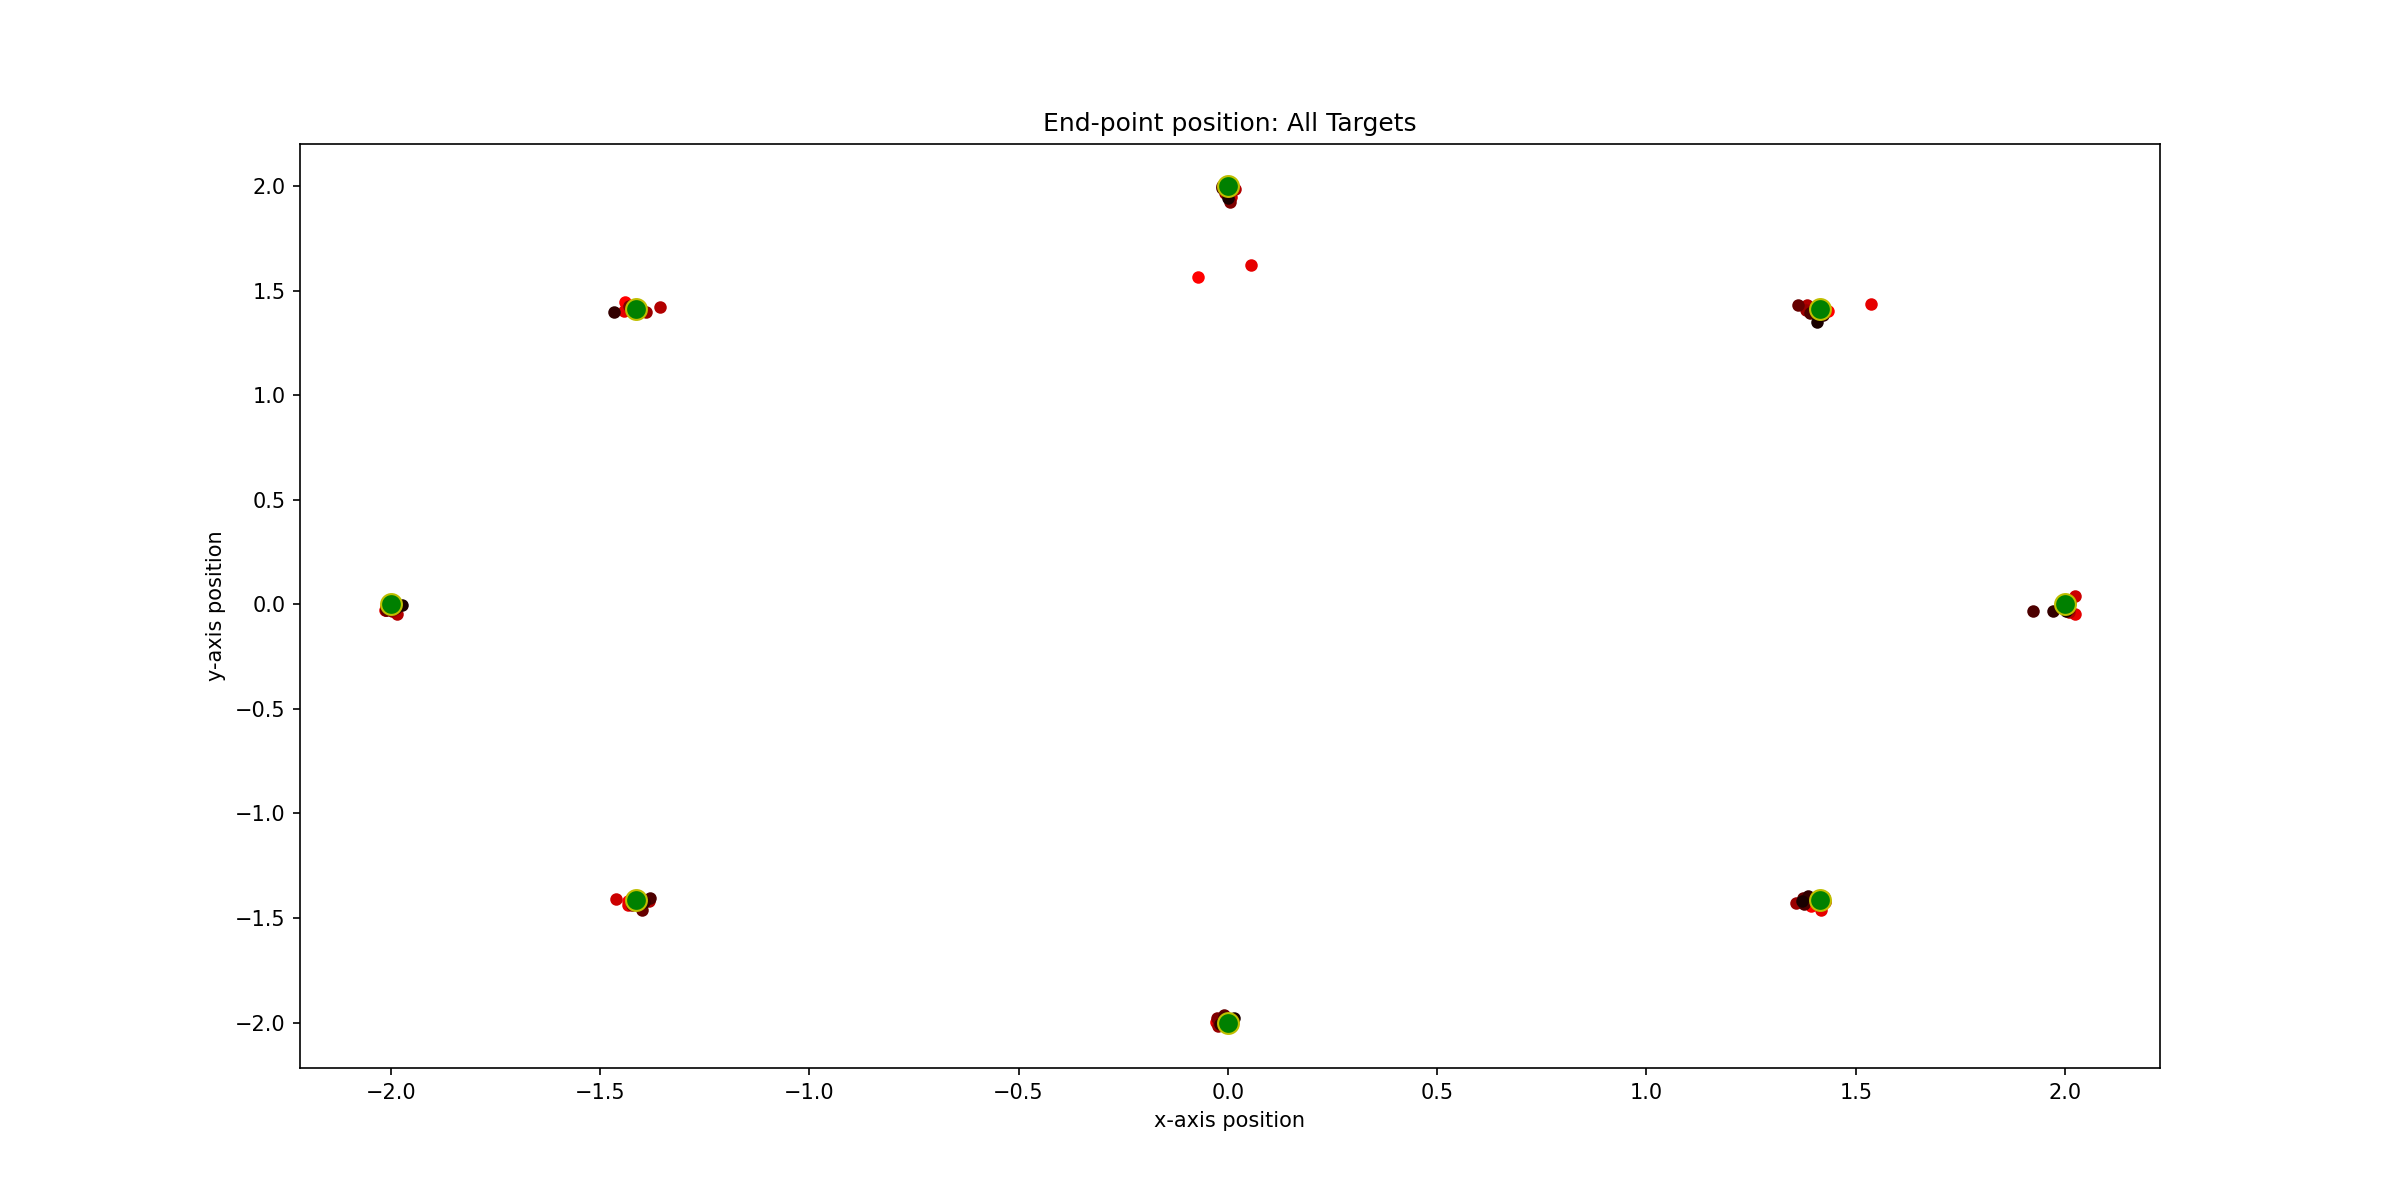
\includegraphics[width=\linewidth]{sujeto1/no_force/trayectorias_puntos}
		\caption{Sujeto 1, sin fuerza}
		\label{fig:figura1}
	\end{minipage}
	\hspace{0.2cm}
	\begin{minipage}[b]{0.5\linewidth}
		\centering
		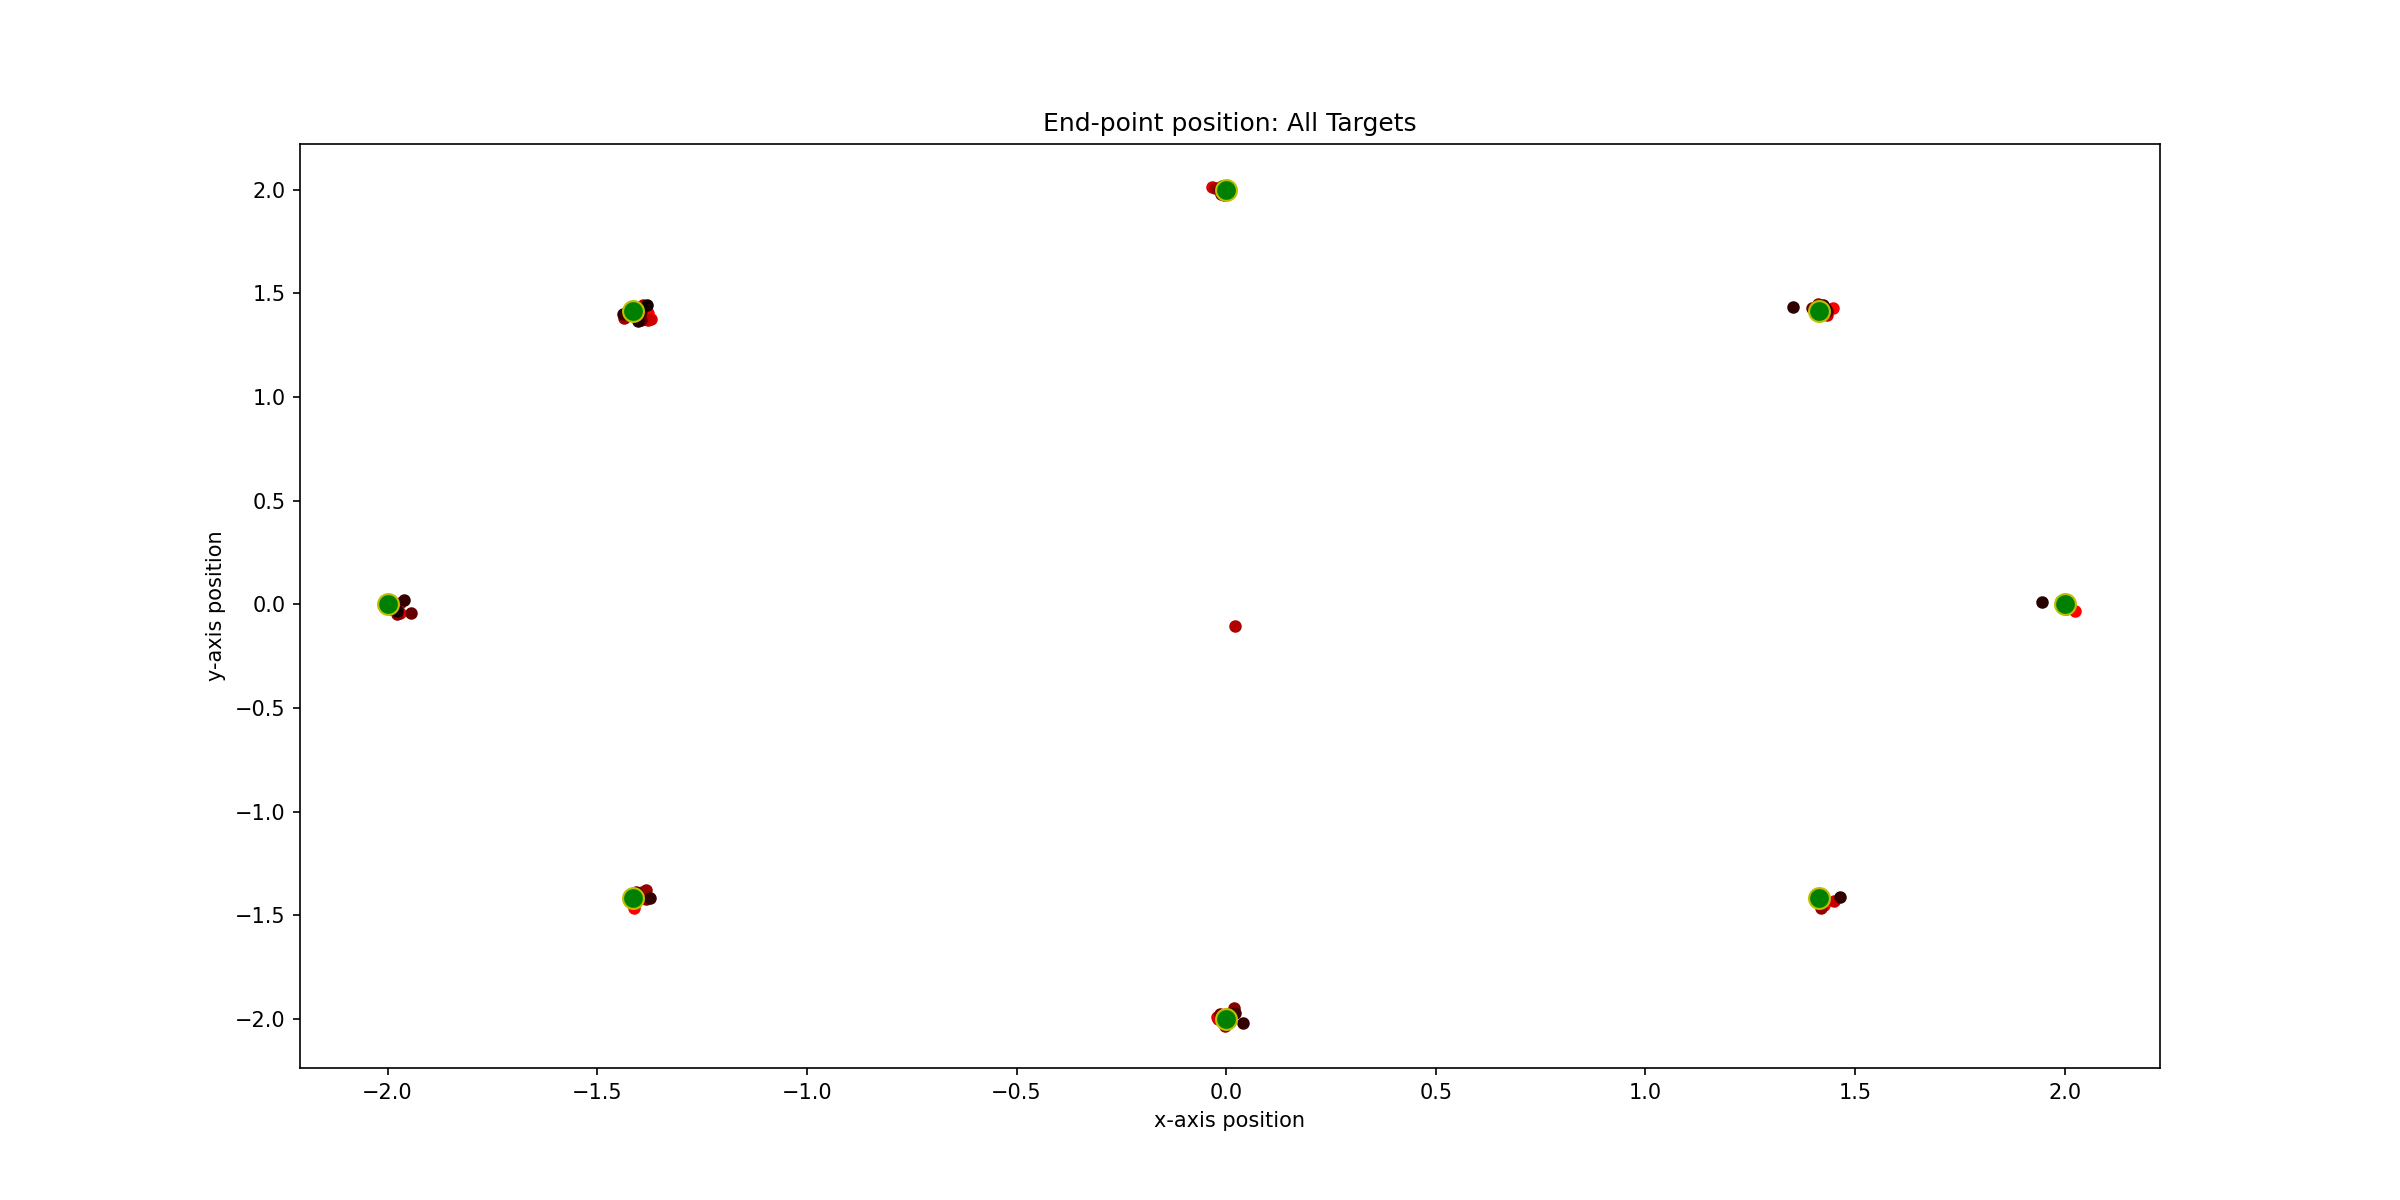
\includegraphics[width=\linewidth]{sujeto2/no_force/trayectorias_puntos}
		\caption{Sujeto 2, sin fuerza}
		\label{fig:figura2}
	\end{minipage}
\end{figure}
\begin{figure}[h]
	\begin{minipage}[b]{0.5\linewidth}
		\centering
		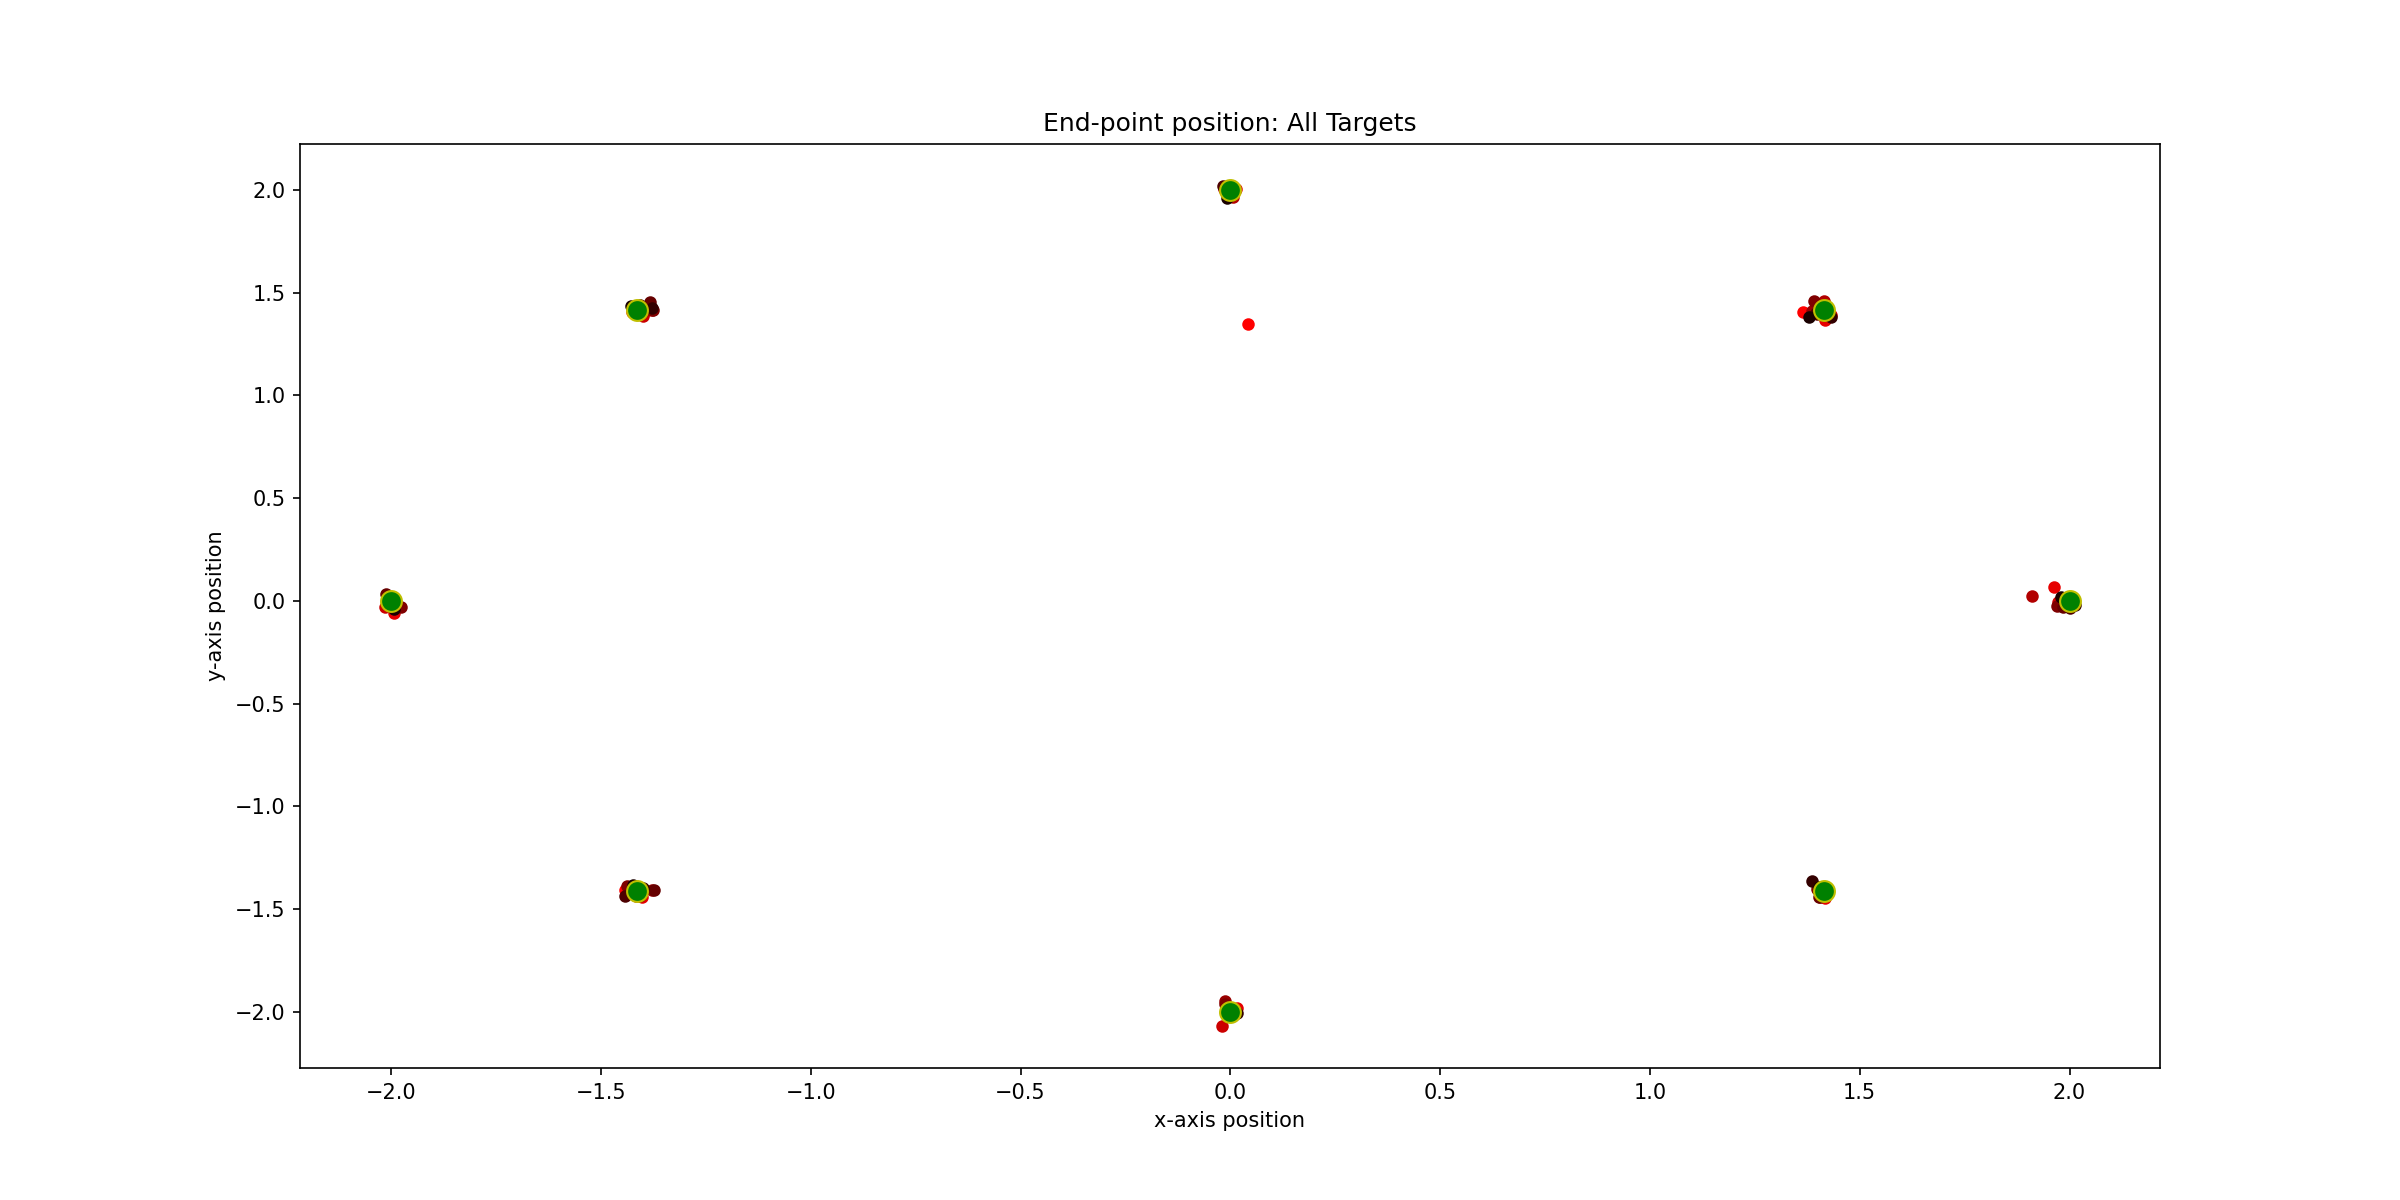
\includegraphics[width=\linewidth]{sujeto4/no_force/trayectorias_puntos}
		\caption{Sujeto 4, sin fuerza}
		\label{fig:figura1}
	\end{minipage}
\end{figure}


Sujetos mayores de 60 años:
\\
\begin{figure}[h]
	\begin{minipage}[b]{0.5\linewidth}
		\centering
		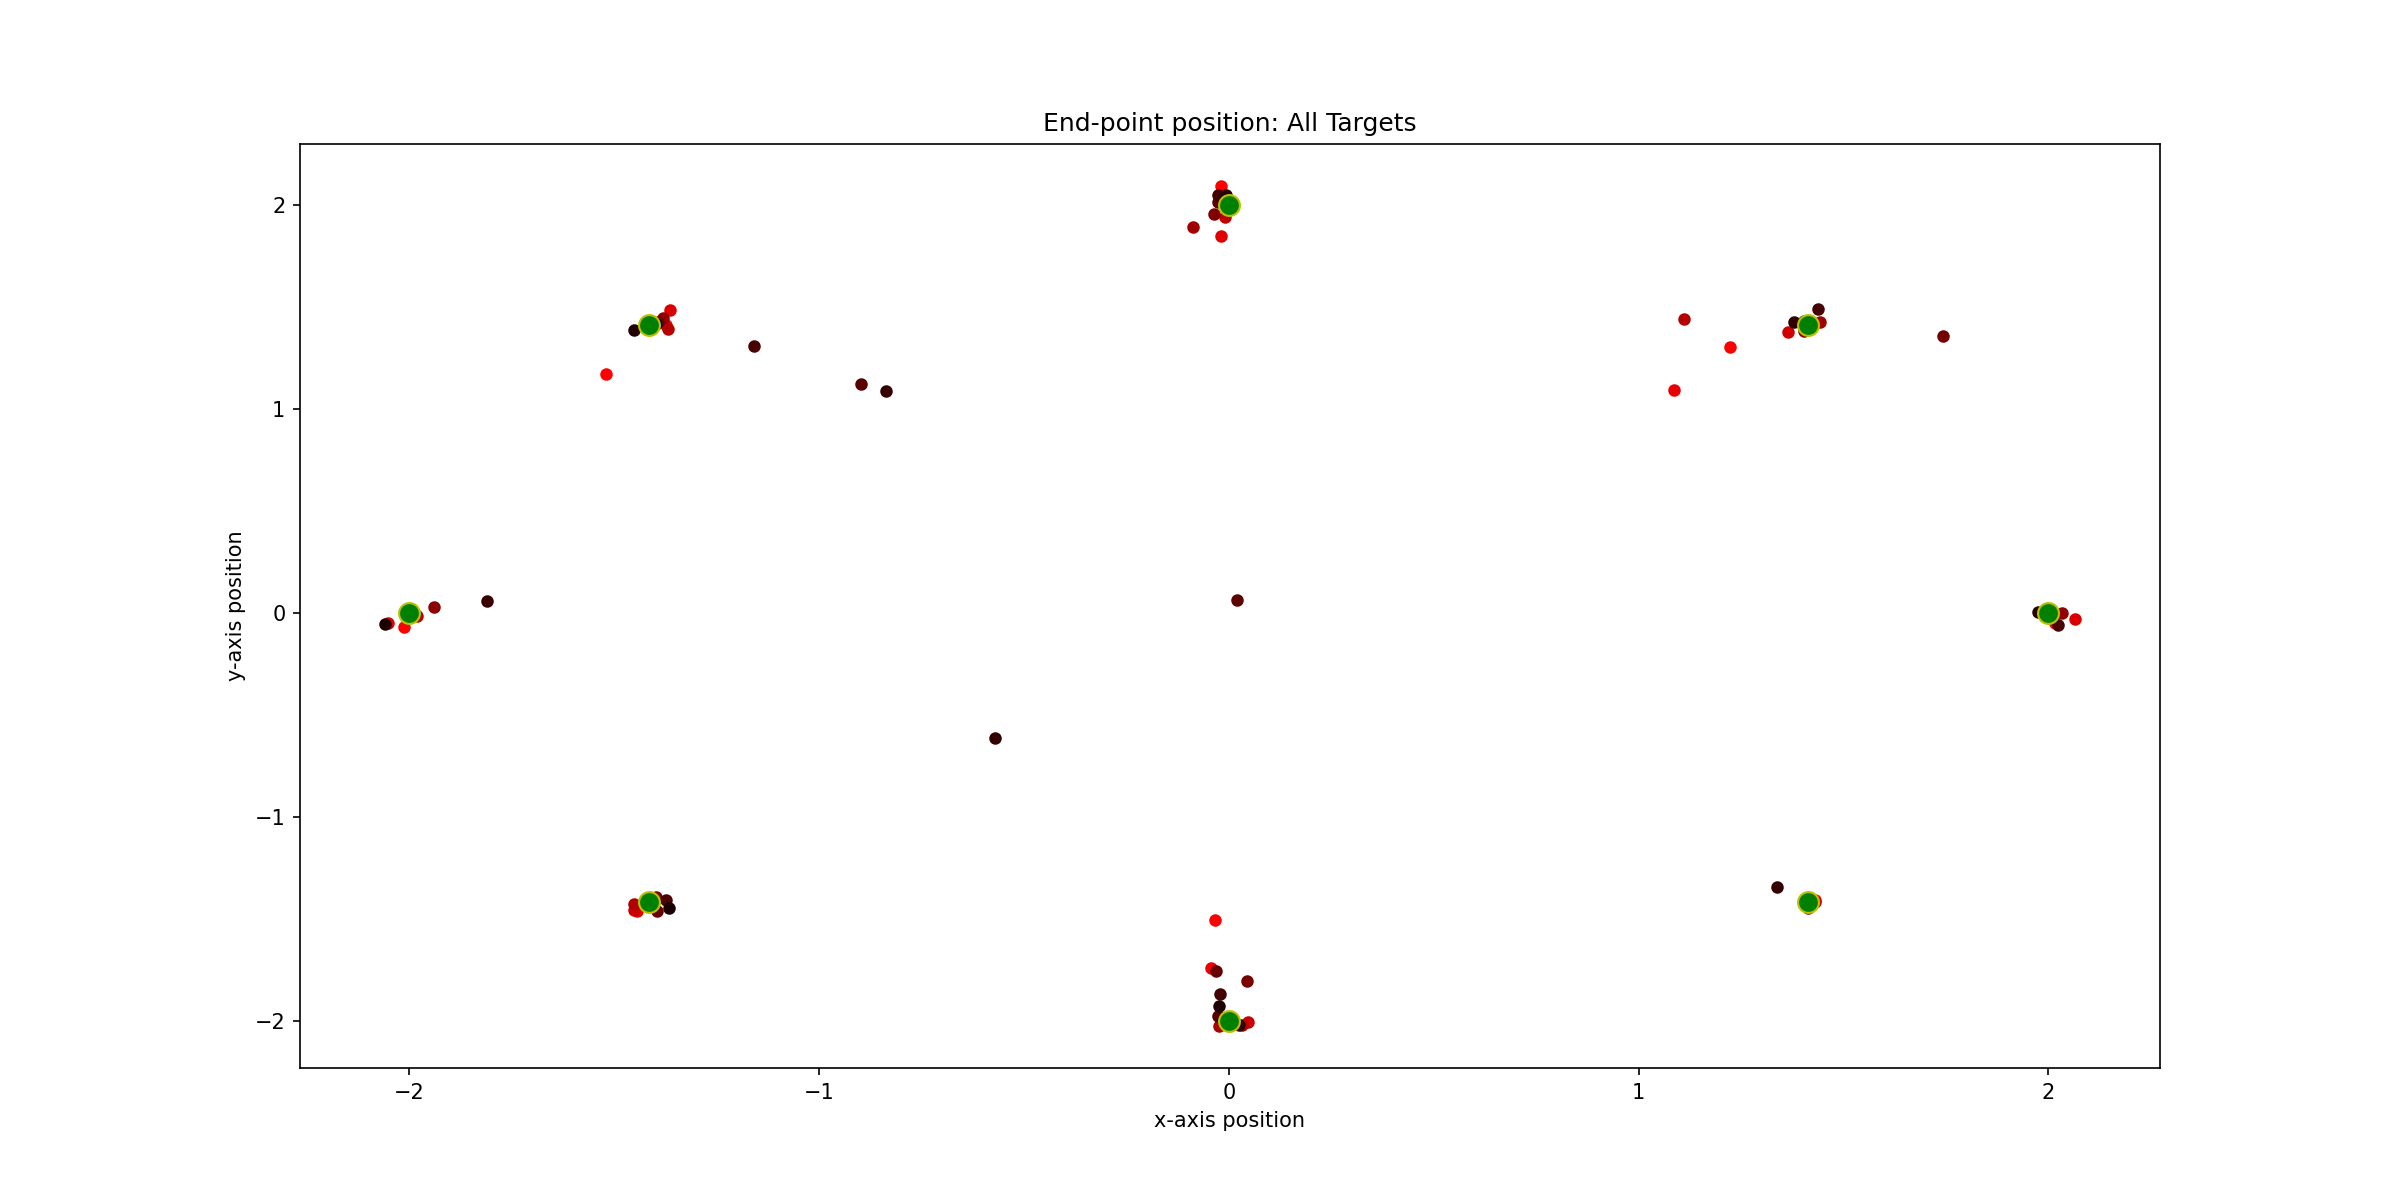
\includegraphics[width=\linewidth]{sujeto3/no_force/trayectorias_puntos}
		\caption{Sujeto 3, sin fuerza}
		\label{fig:figura1}
	\end{minipage}
	\hspace{0.5cm}
	\begin{minipage}[b]{0.5\linewidth}
		\centering
		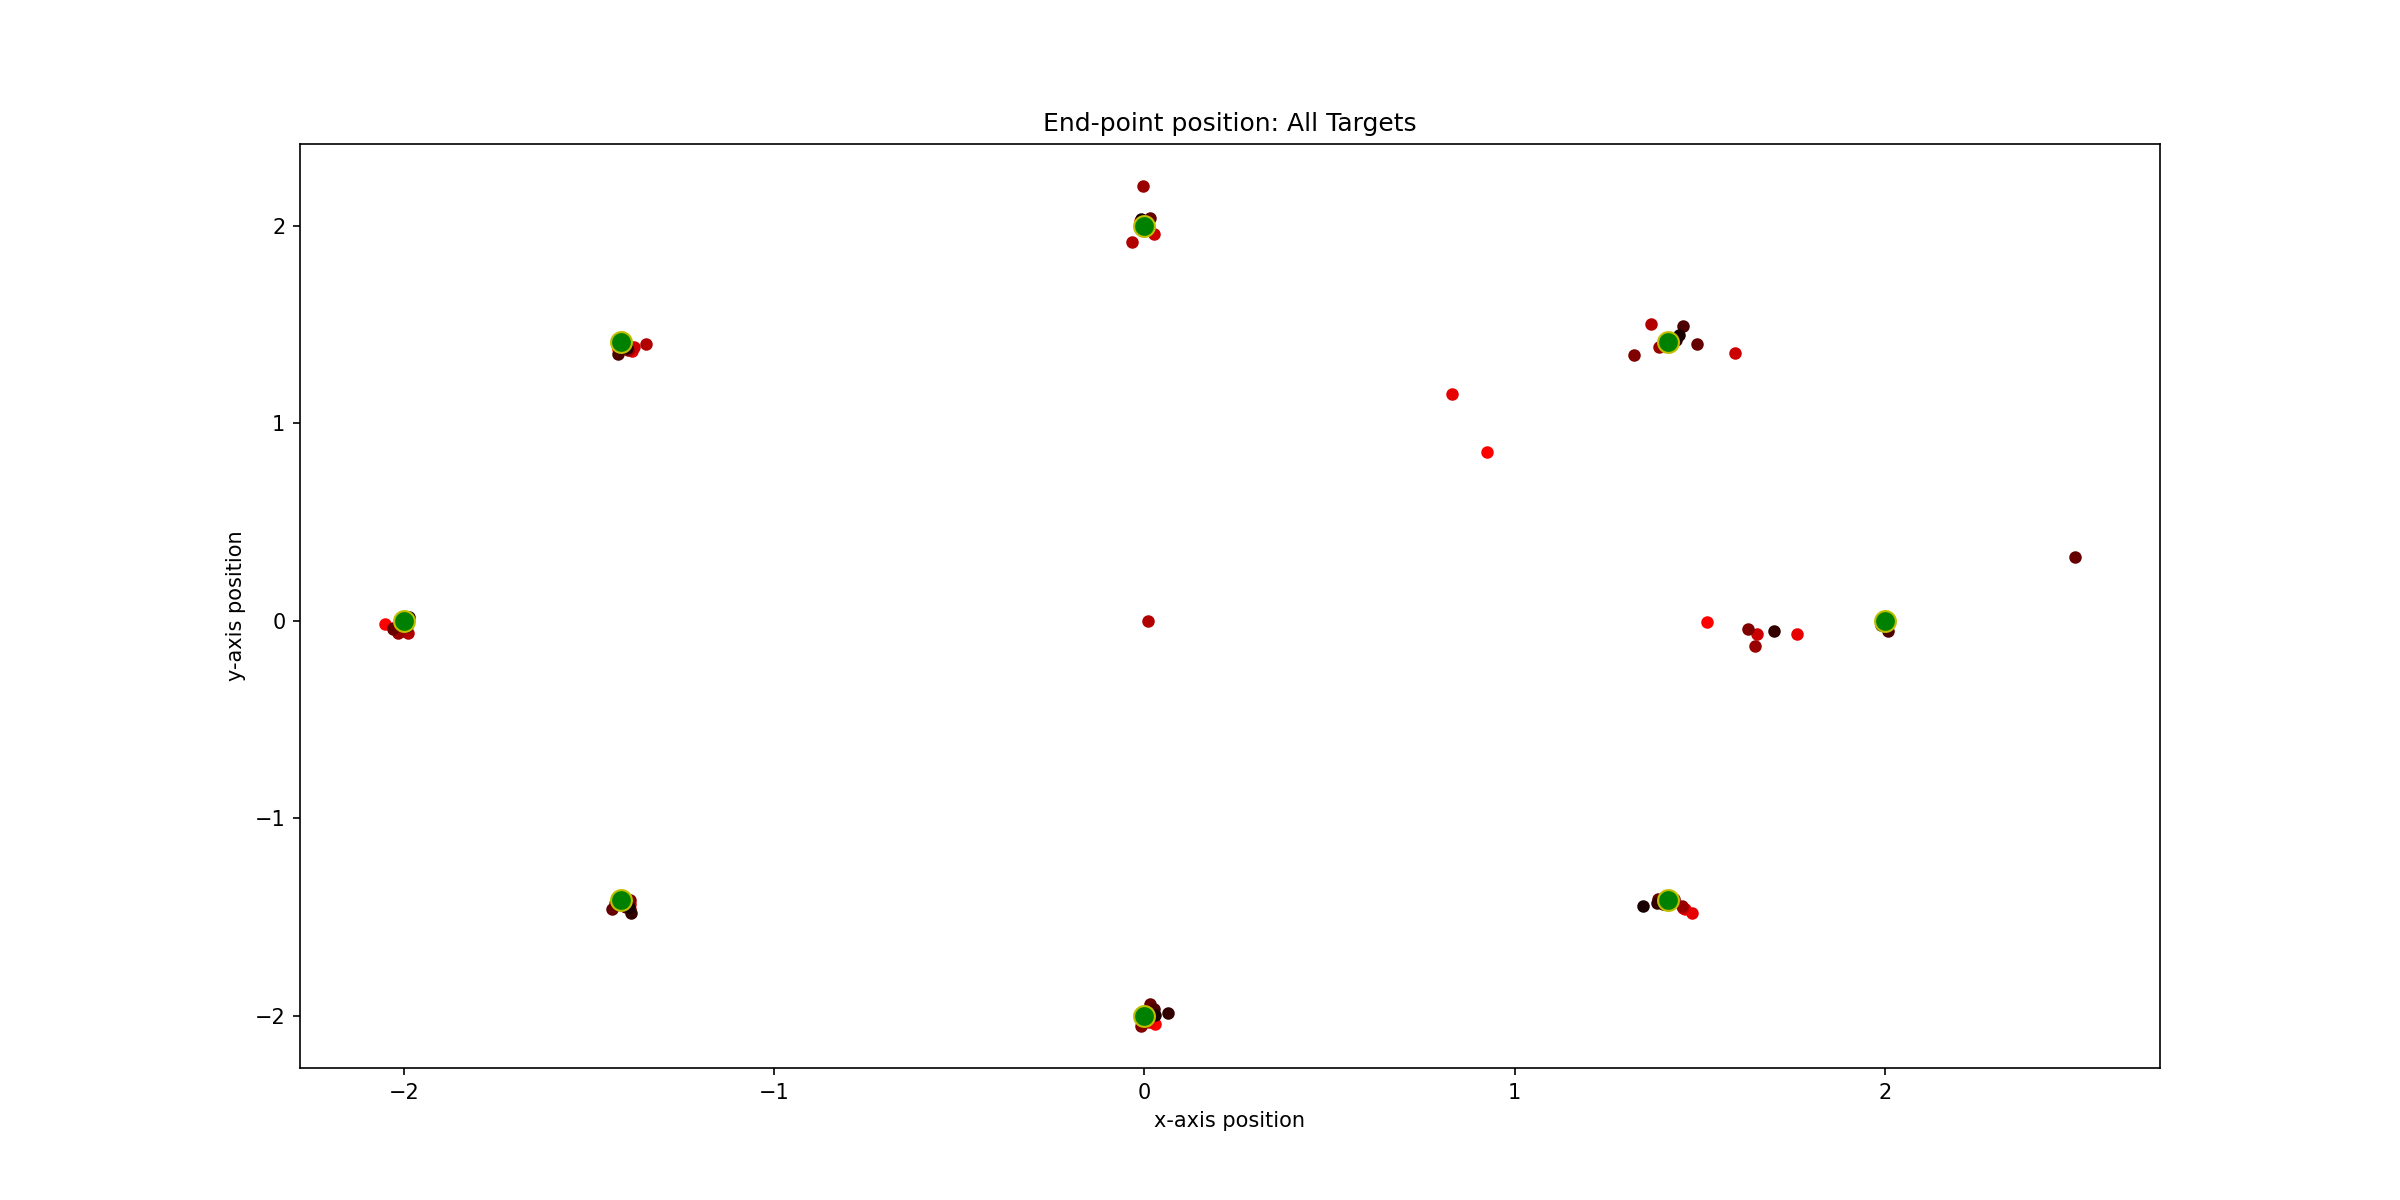
\includegraphics[width=\linewidth]{sujeto5/no_force/trayectorias_puntos}
		\caption{Sujeto 5, sin fuerza}
		\label{fig:figura2}
	\end{minipage}
\end{figure}

También lo podemos ver en las siguientes gráficas, donde ademas observamos que el proceso de aprendizaje en los sujetos jóvenes es casi instantáneo, mientras que en las personas mayores, en el caso de sujeto 2 (en orden) se aprecia un aprendizaje en los primeros puntos objetivos (T1 y T2) que luego se extrapola a los demás puntos, mientras que en el sujeto 3 (aleatorio) ese aprendizaje es más incierto.

Sujetos más jóvenes:
\\
\begin{figure}[h]
	\begin{minipage}[b]{0.5\linewidth}
		\centering
		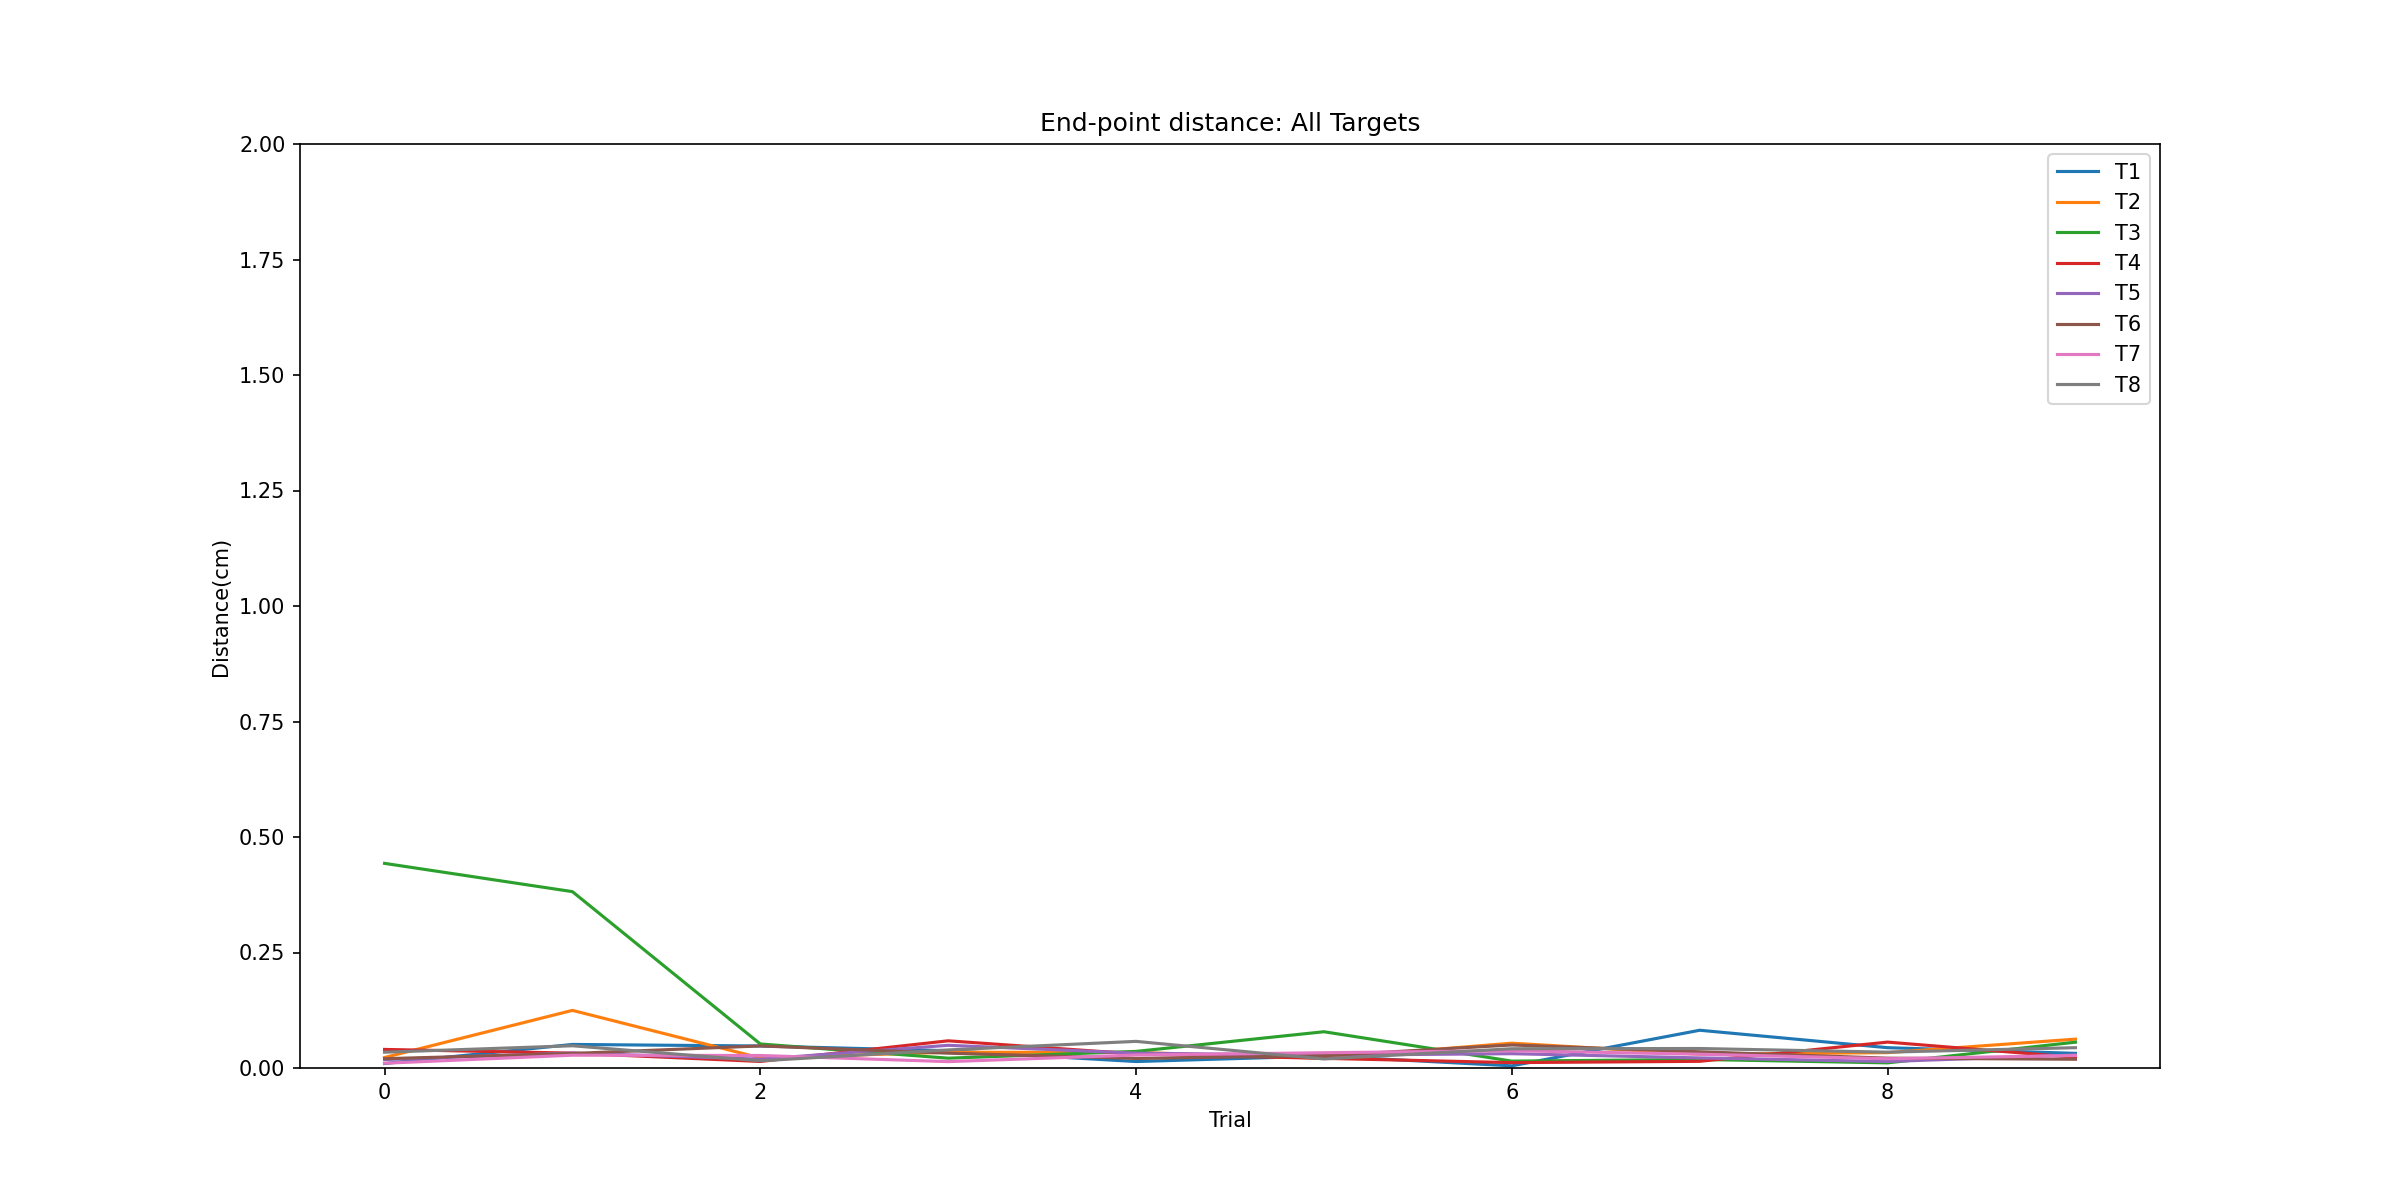
\includegraphics[width=\linewidth]{sujeto1/no_force/evolution_distance}
		\caption{Sujeto 1, sin fuerza}
		\label{fig:figura1}
	\end{minipage}
	\hspace{0.5cm}
	\begin{minipage}[b]{0.5\linewidth}
		\centering
		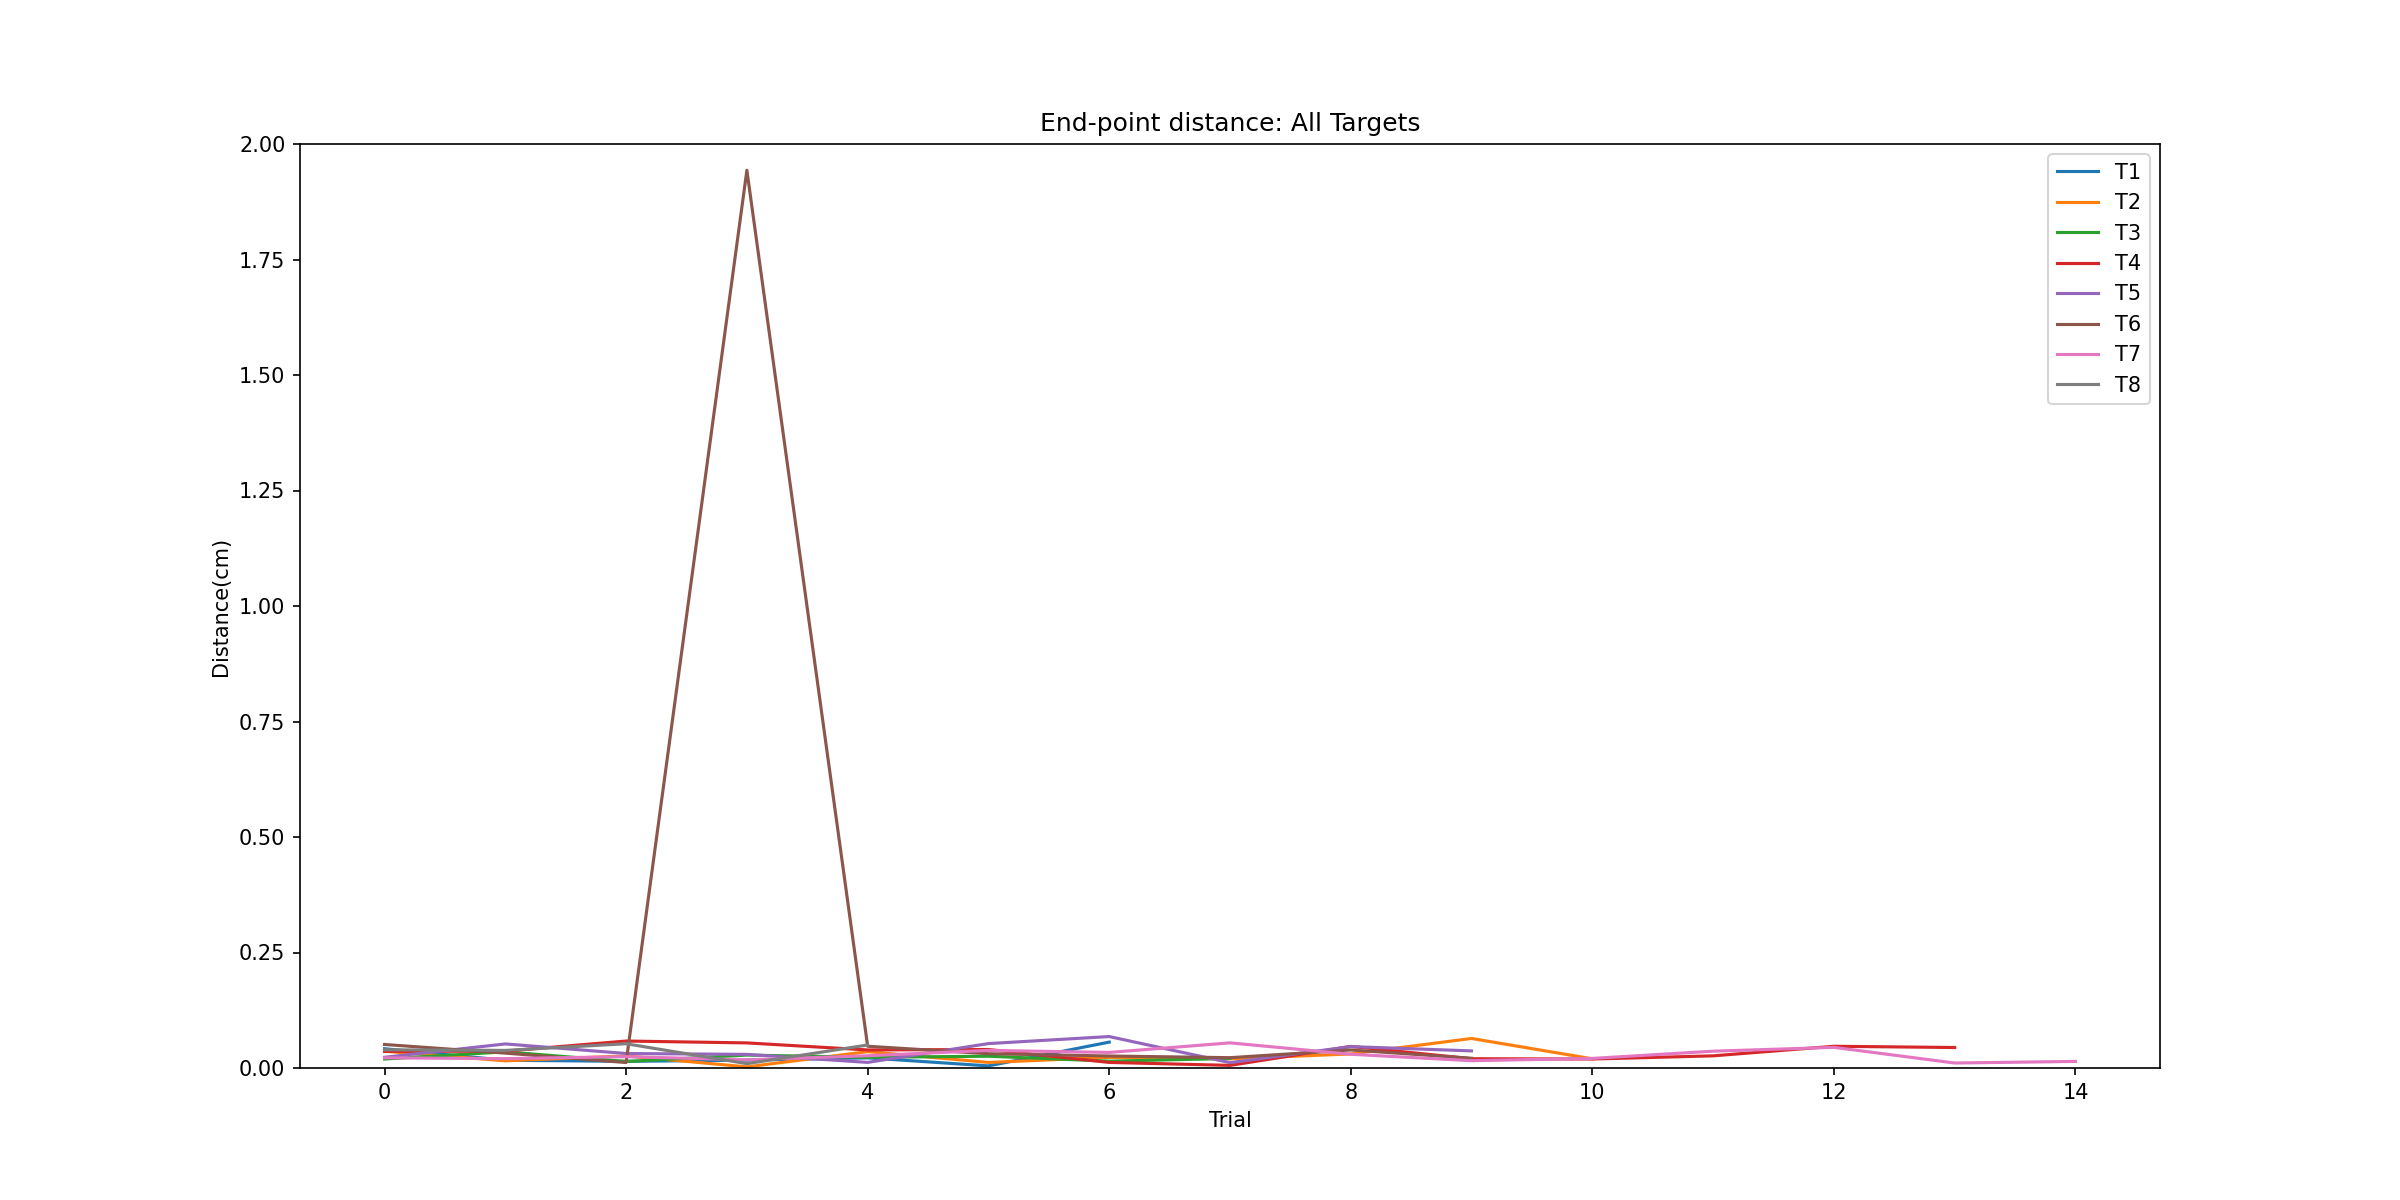
\includegraphics[width=\linewidth]{sujeto2/no_force/evolution_distance}
		\caption{Sujeto 2, sin fuerza}
		\label{fig:figura2}
	\end{minipage}
\end{figure}
\begin{figure}[h]
	\begin{minipage}[b]{0.5\linewidth}
		\centering
		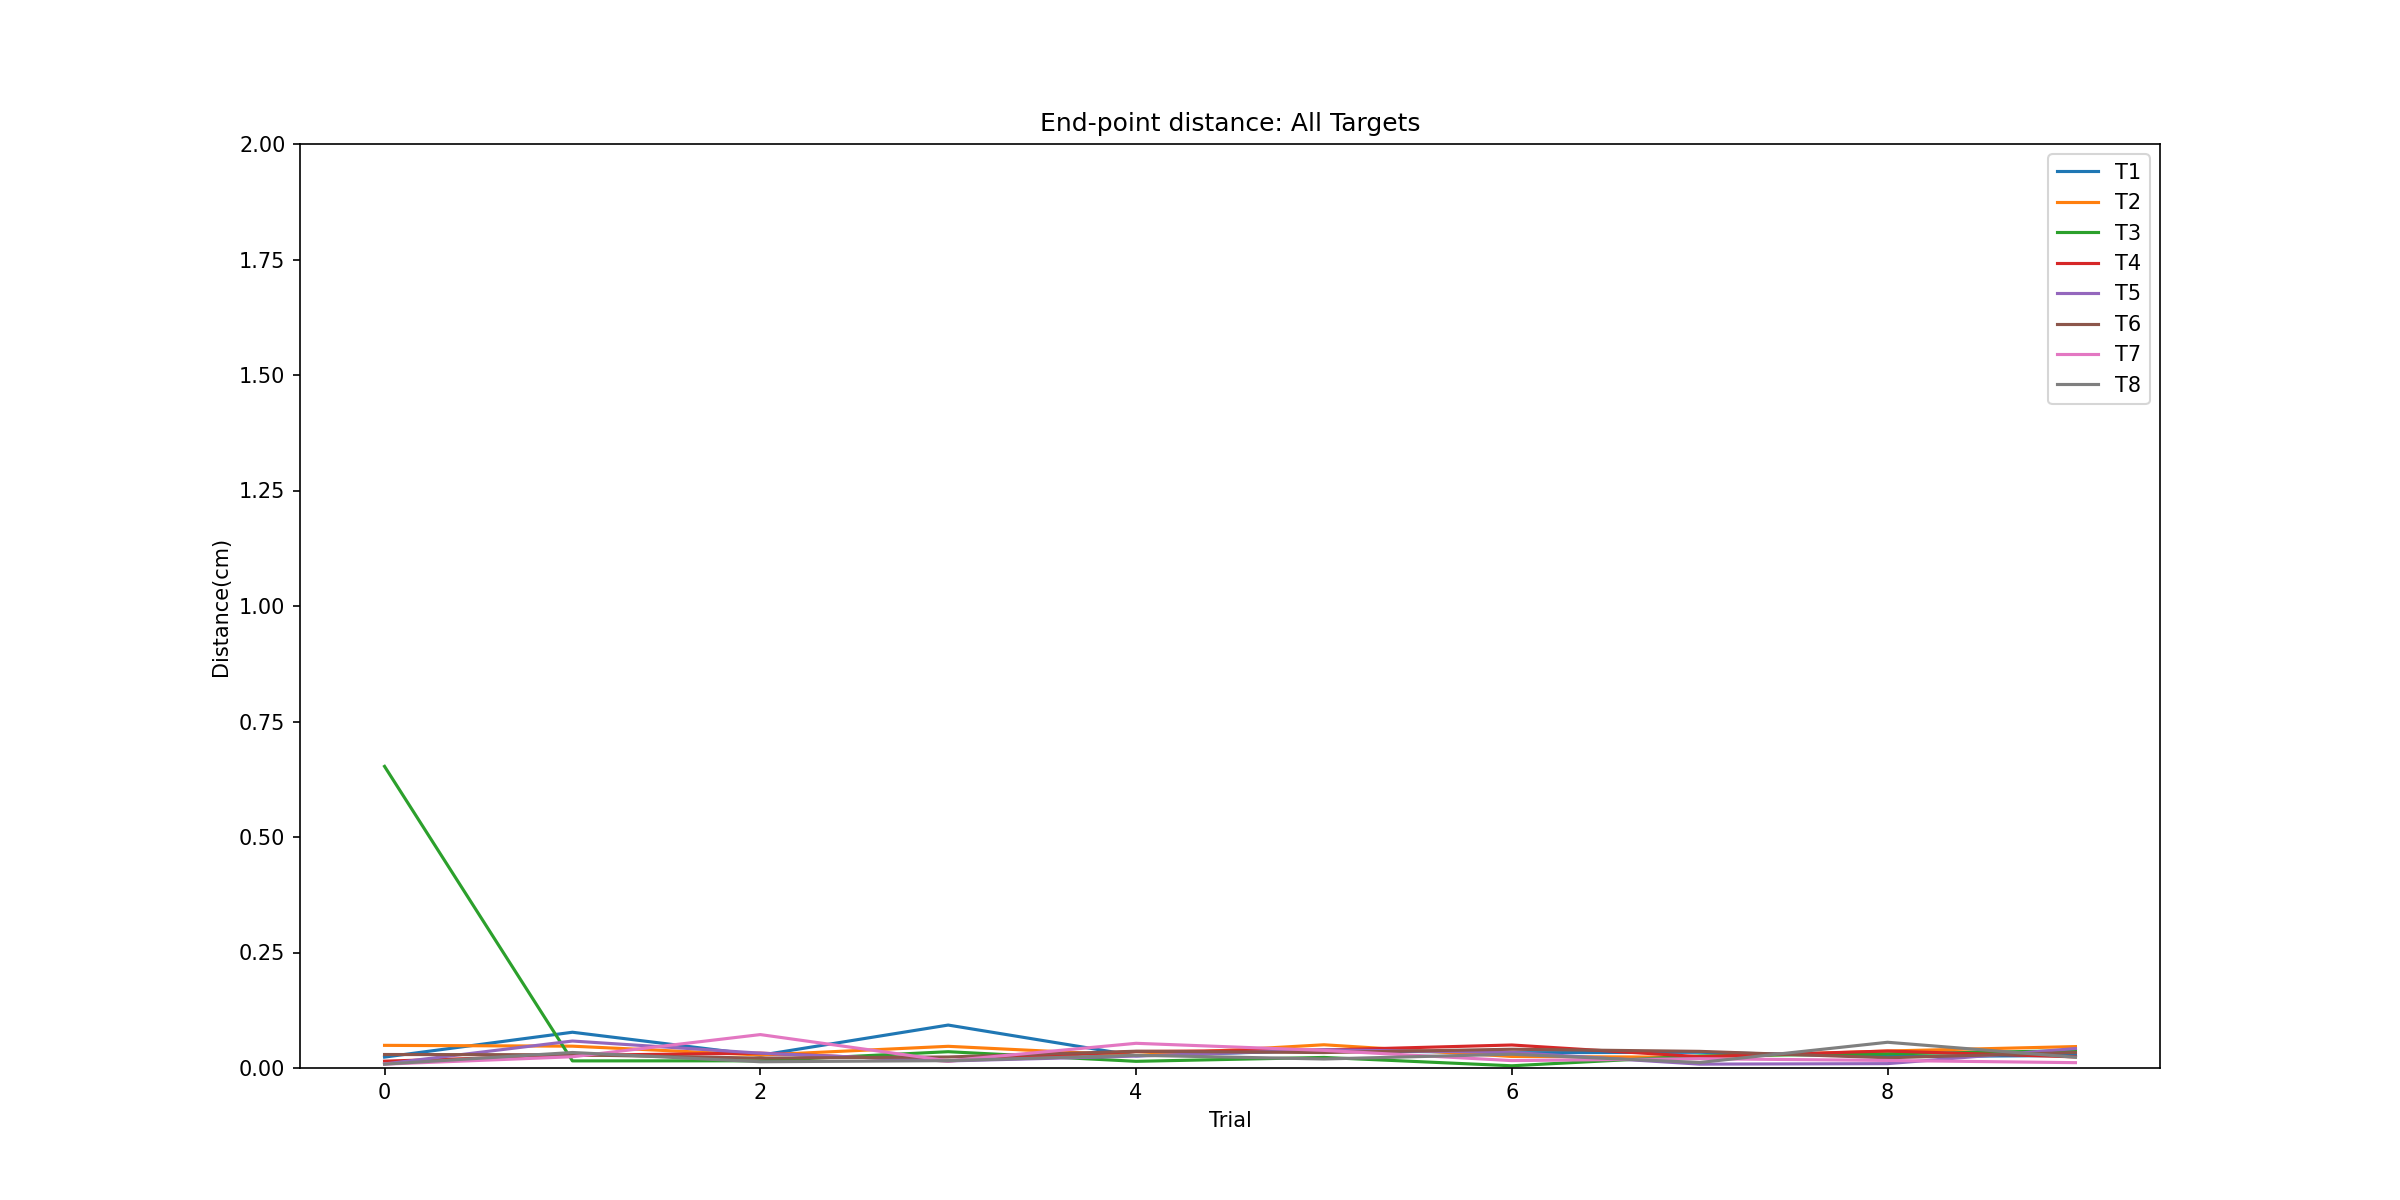
\includegraphics[width=\linewidth]{sujeto4/no_force/evolution_distance}
		\caption{Sujeto 4, sin fuerza}
		\label{fig:figura1}
	\end{minipage}
\end{figure}


Sujetos mayores de 60 años:
\\
\begin{figure}[h]
	\begin{minipage}[b]{0.5\linewidth}
		\centering
		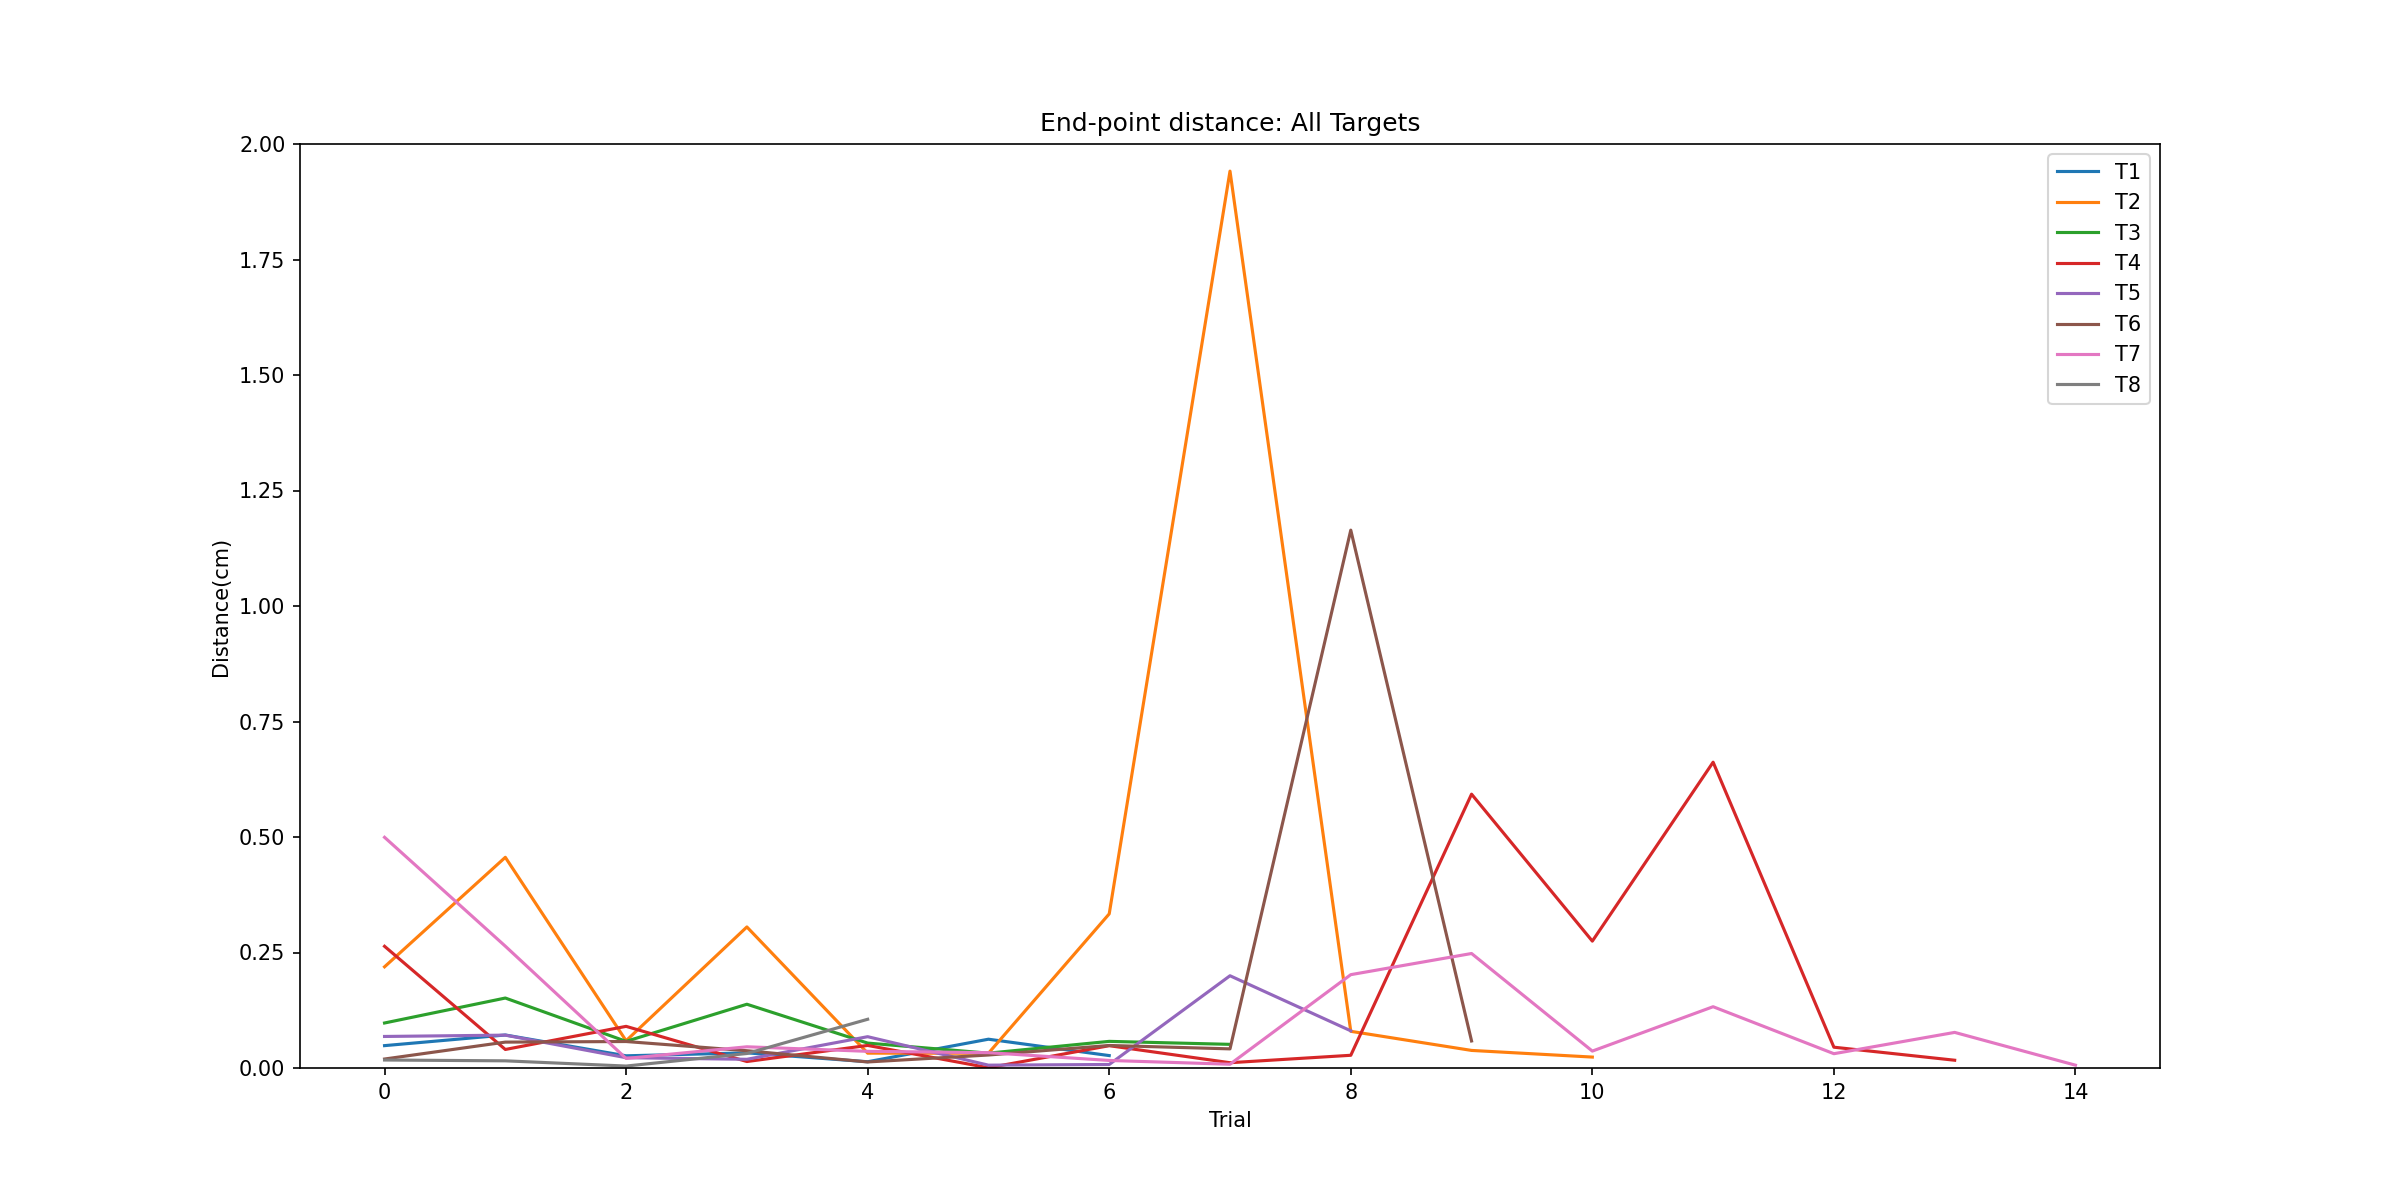
\includegraphics[width=\linewidth]{sujeto3/no_force/evolution_distance}
		\caption{Sujeto 3, sin fuerza}
		\label{fig:figura1}
	\end{minipage}
	\hspace{0.5cm}
	\begin{minipage}[b]{0.5\linewidth}
		\centering
		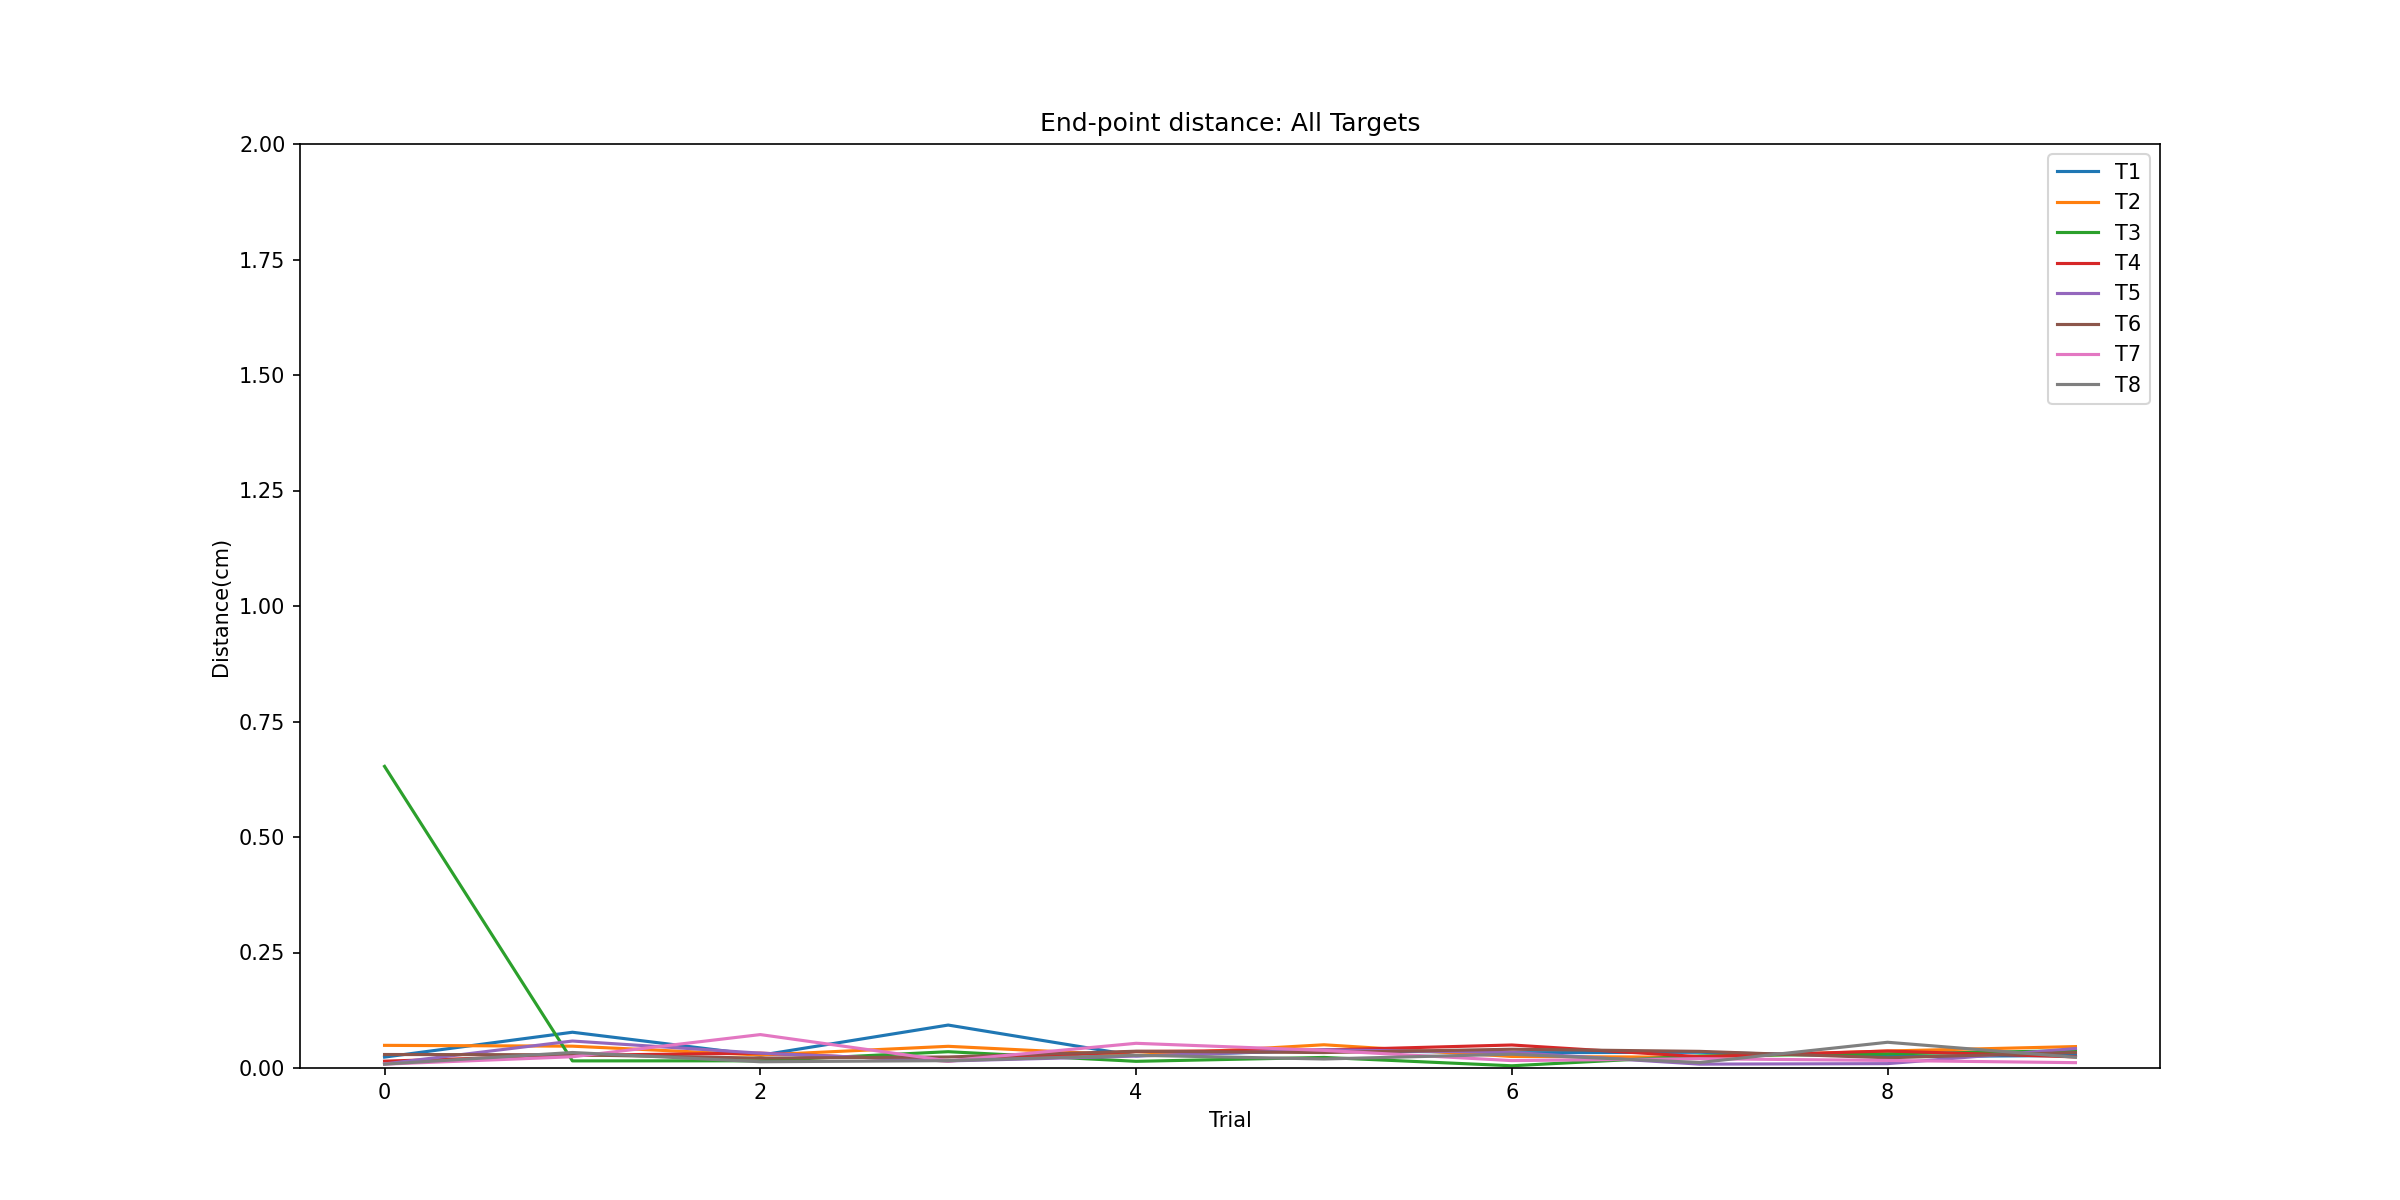
\includegraphics[width=\linewidth]{sujeto4/no_force/evolution_distance}
		\caption{Sujeto 5, sin fuerza}
		\label{fig:figura2}
	\end{minipage}
\end{figure}


Si además estudiamos la rapidez en la ejecución de los movimientos podemos ver que el sujeto que peor lo hace es el 3 (persona mayor, aleatorio), y el mejor el sujeto 4 (50 años, en orden). Podemos ver que, aunque los sujetos 3 y 5 tienen una tasa de errores similar, en el sujeto 5 podemos reconocer un aprendizaje en la rapidez del movimiento (T1 y T2 empiezan a mejorar en las últimas iteraciones y los demás movimientos comienzan a ser más rápidos, especialmente T5 y T7, donde podemos observar una curva casi completamente descendente). Sin embargo en el sujeto 	3 con los puntos en orden aleatorio no lo podemos apreciar, y los tiempos de ejecución son mayores.

\begin{figure}[h]
	\begin{minipage}[b]{0.5\linewidth}
		\centering
		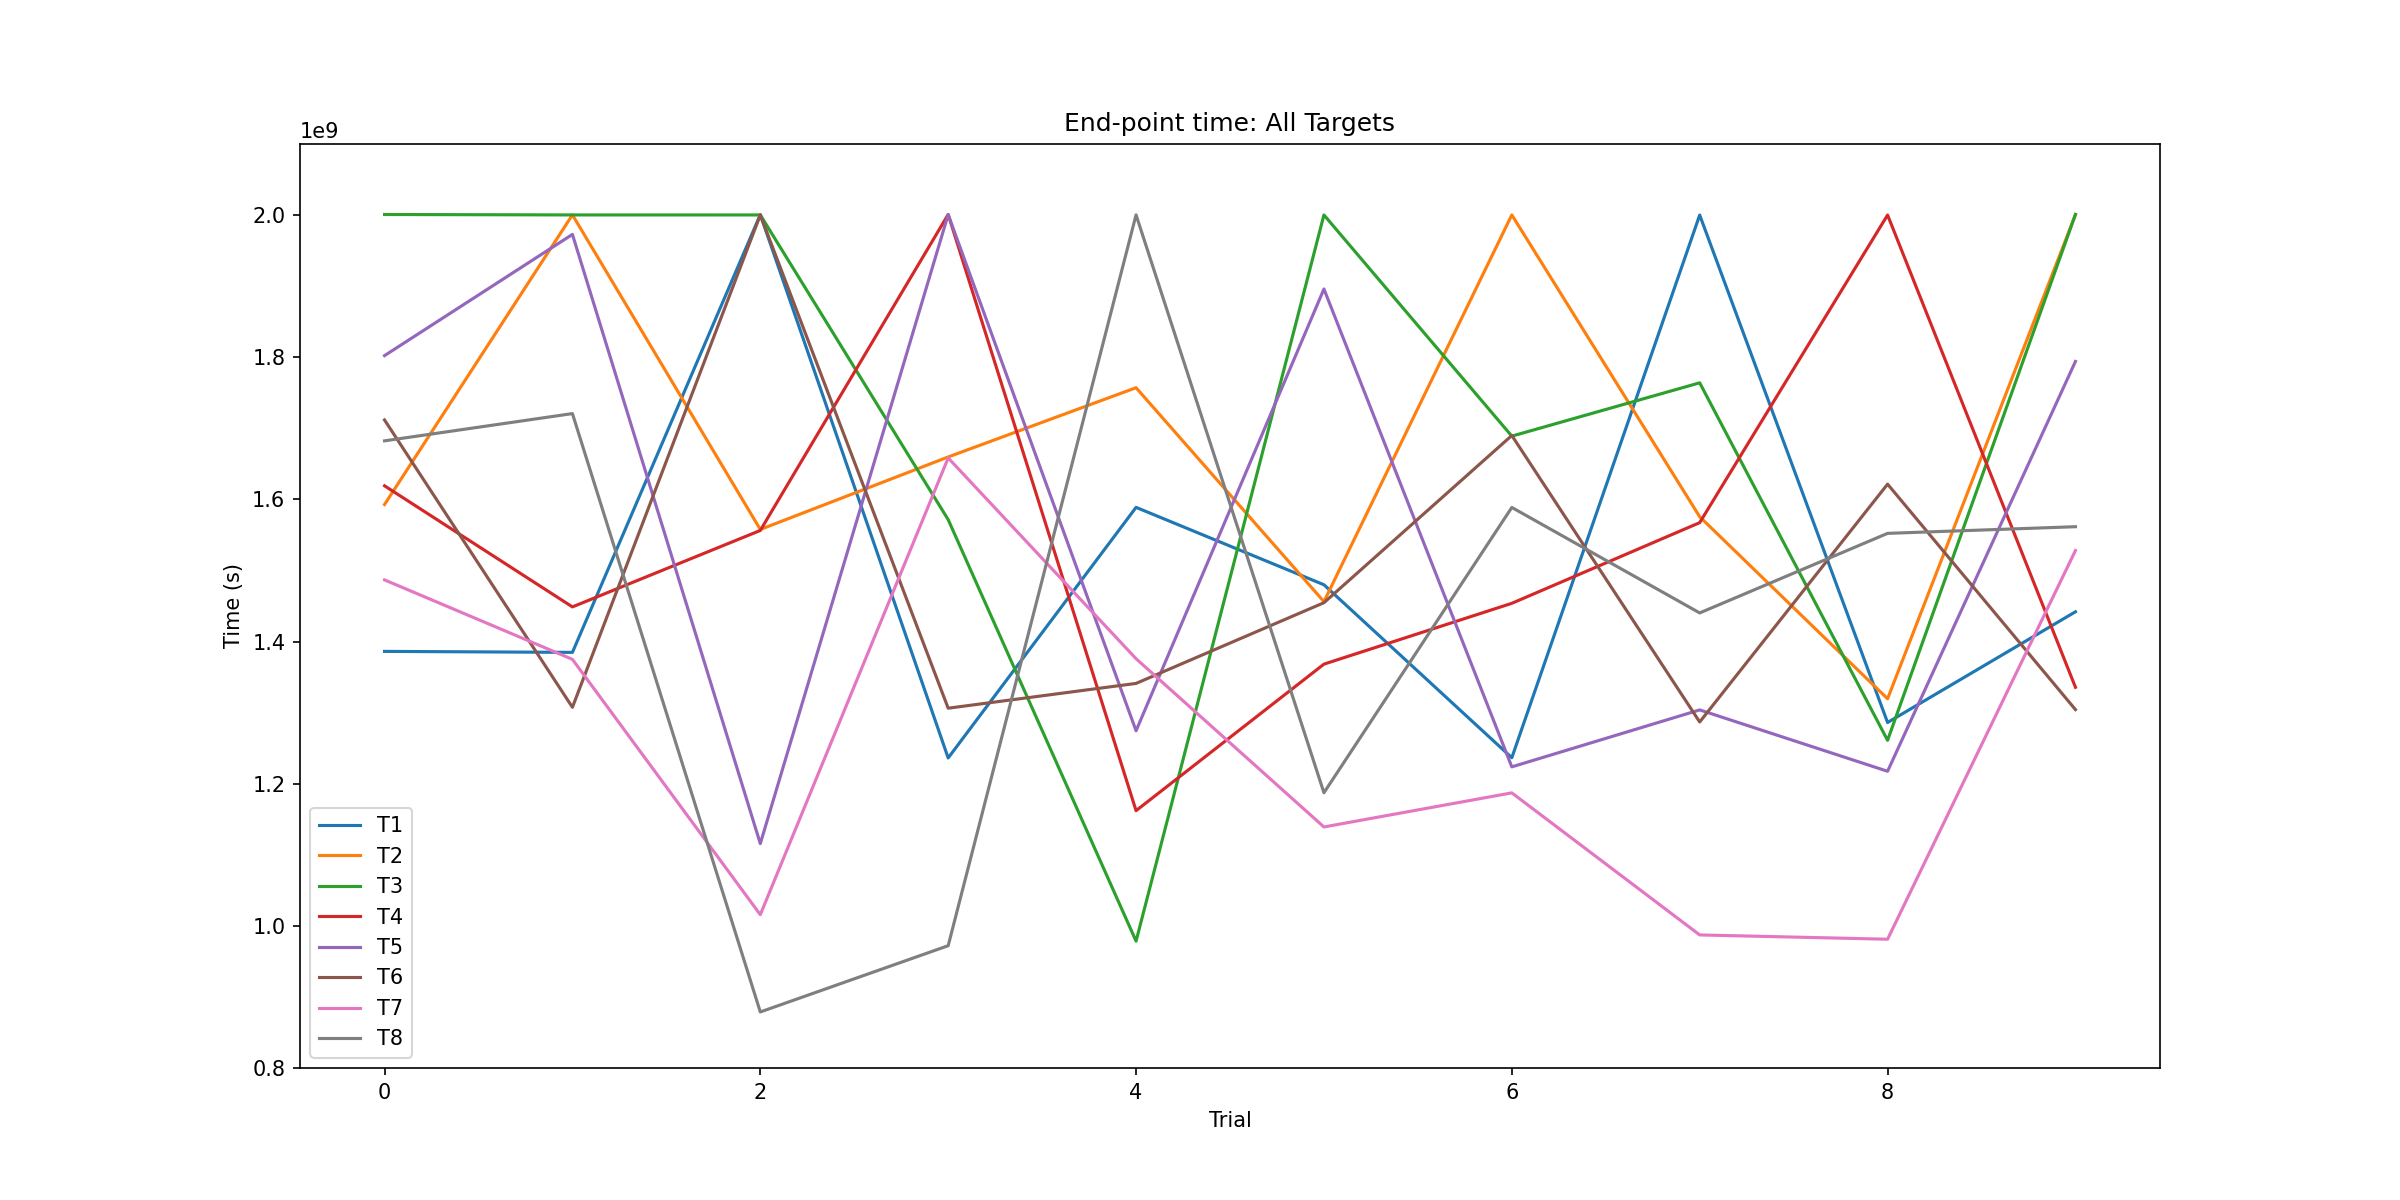
\includegraphics[width=\linewidth]{sujeto1/no_force/evolution_time}
		\caption{Sujeto 1, sin fuerza}
		\label{fig:figura1}
	\end{minipage}
	\hspace{0.5cm}
	\begin{minipage}[b]{0.5\linewidth}
		\centering
		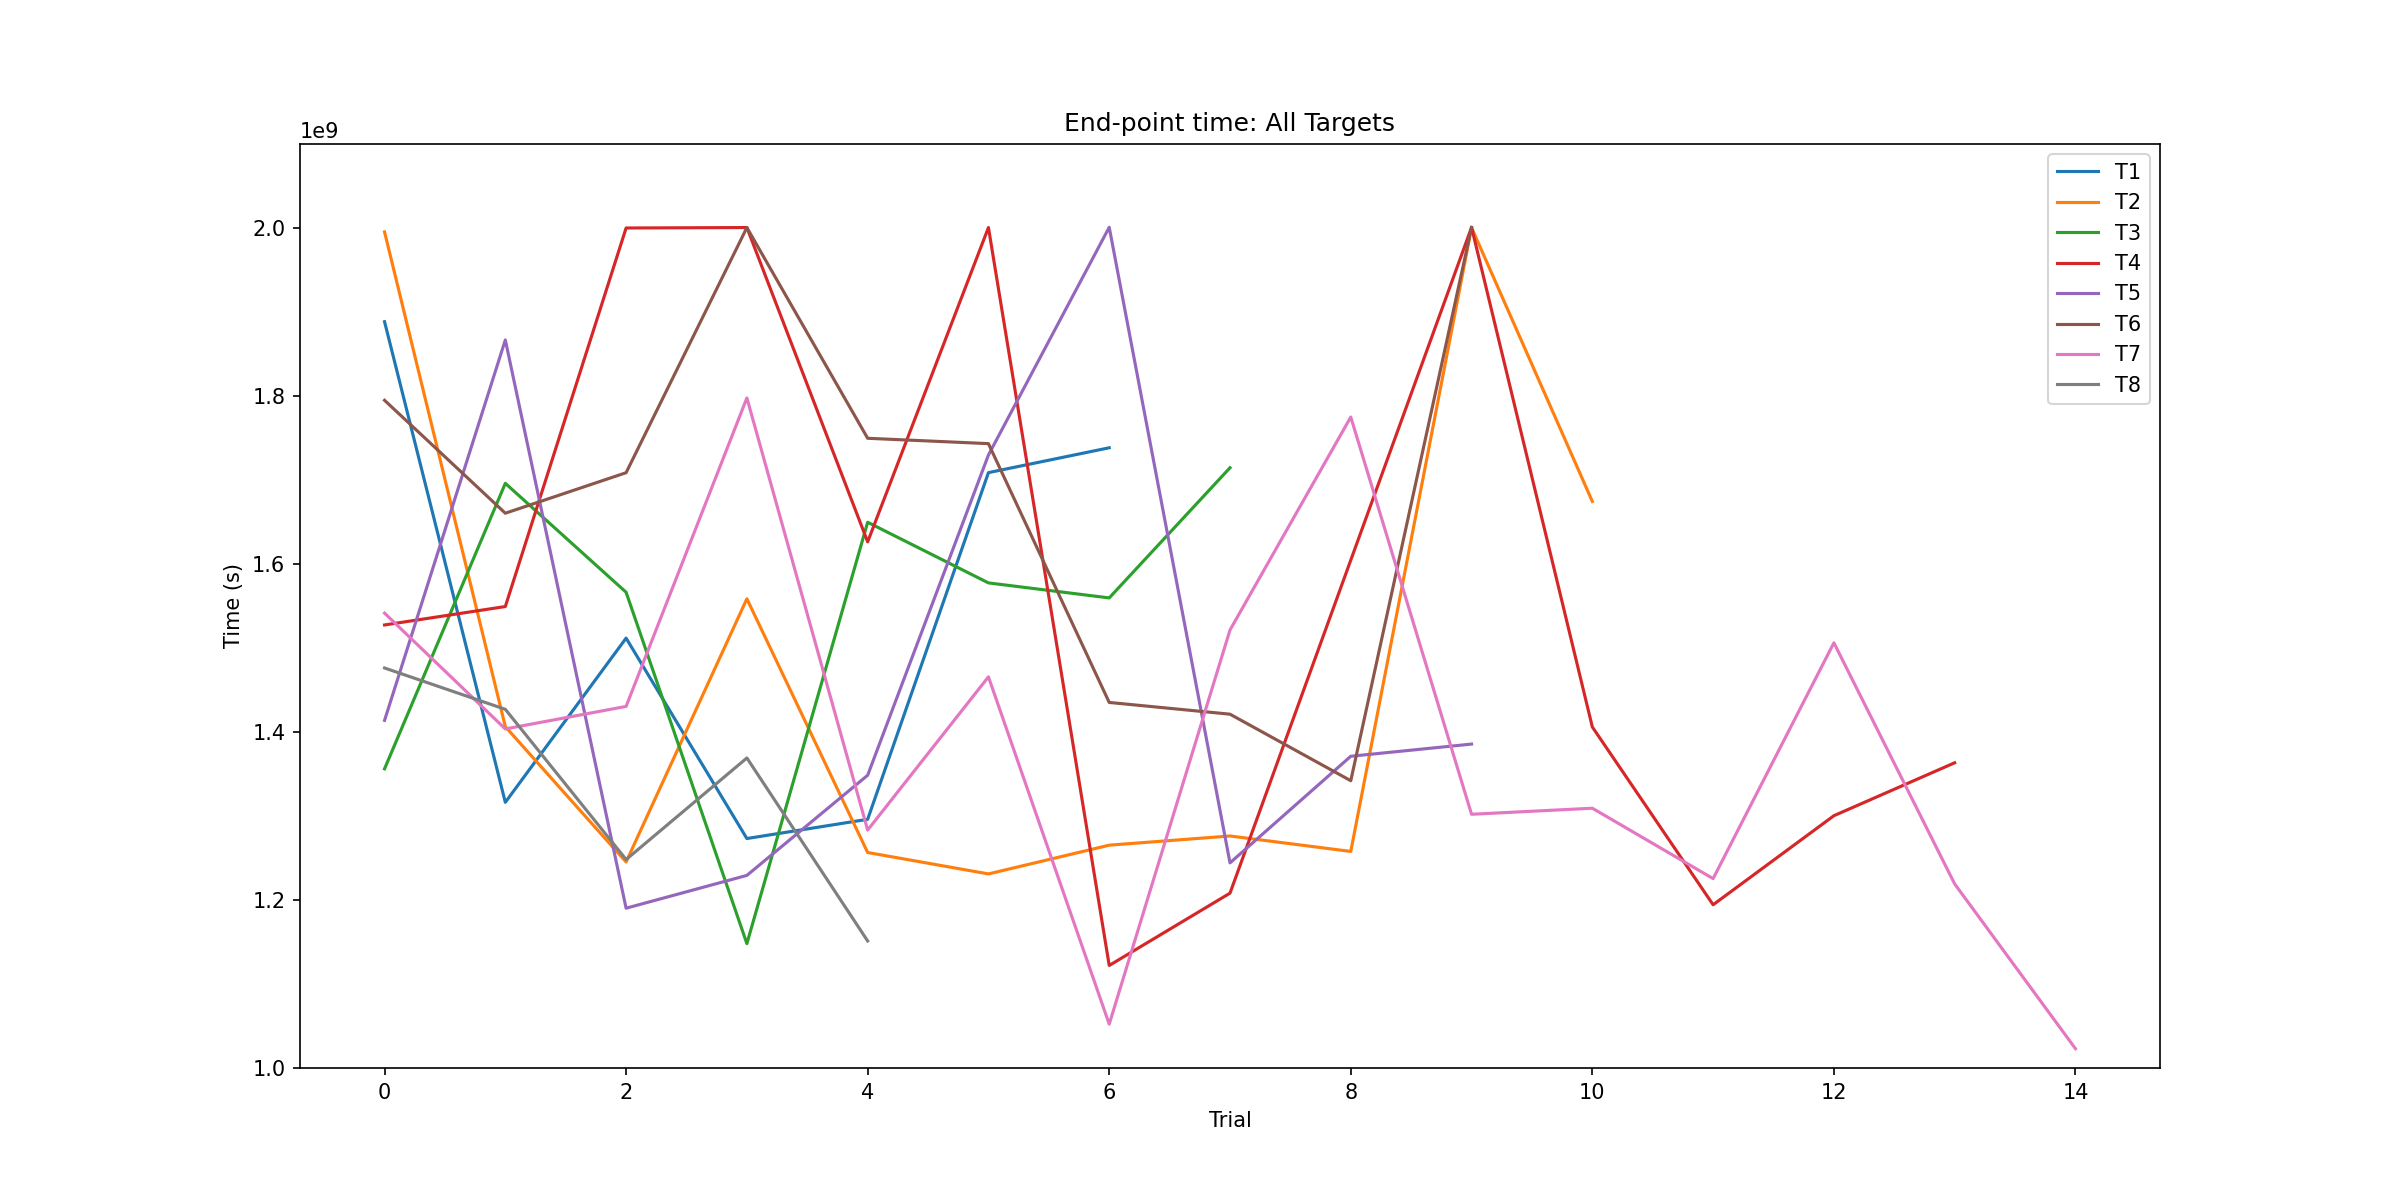
\includegraphics[width=\linewidth]{sujeto2/no_force/evolution_time}
		\caption{Sujeto 2, sin fuerza}
		\label{fig:figura2}
	\end{minipage}
\end{figure}
\begin{figure}[h]
	\begin{minipage}[b]{0.5\linewidth}
		\centering
		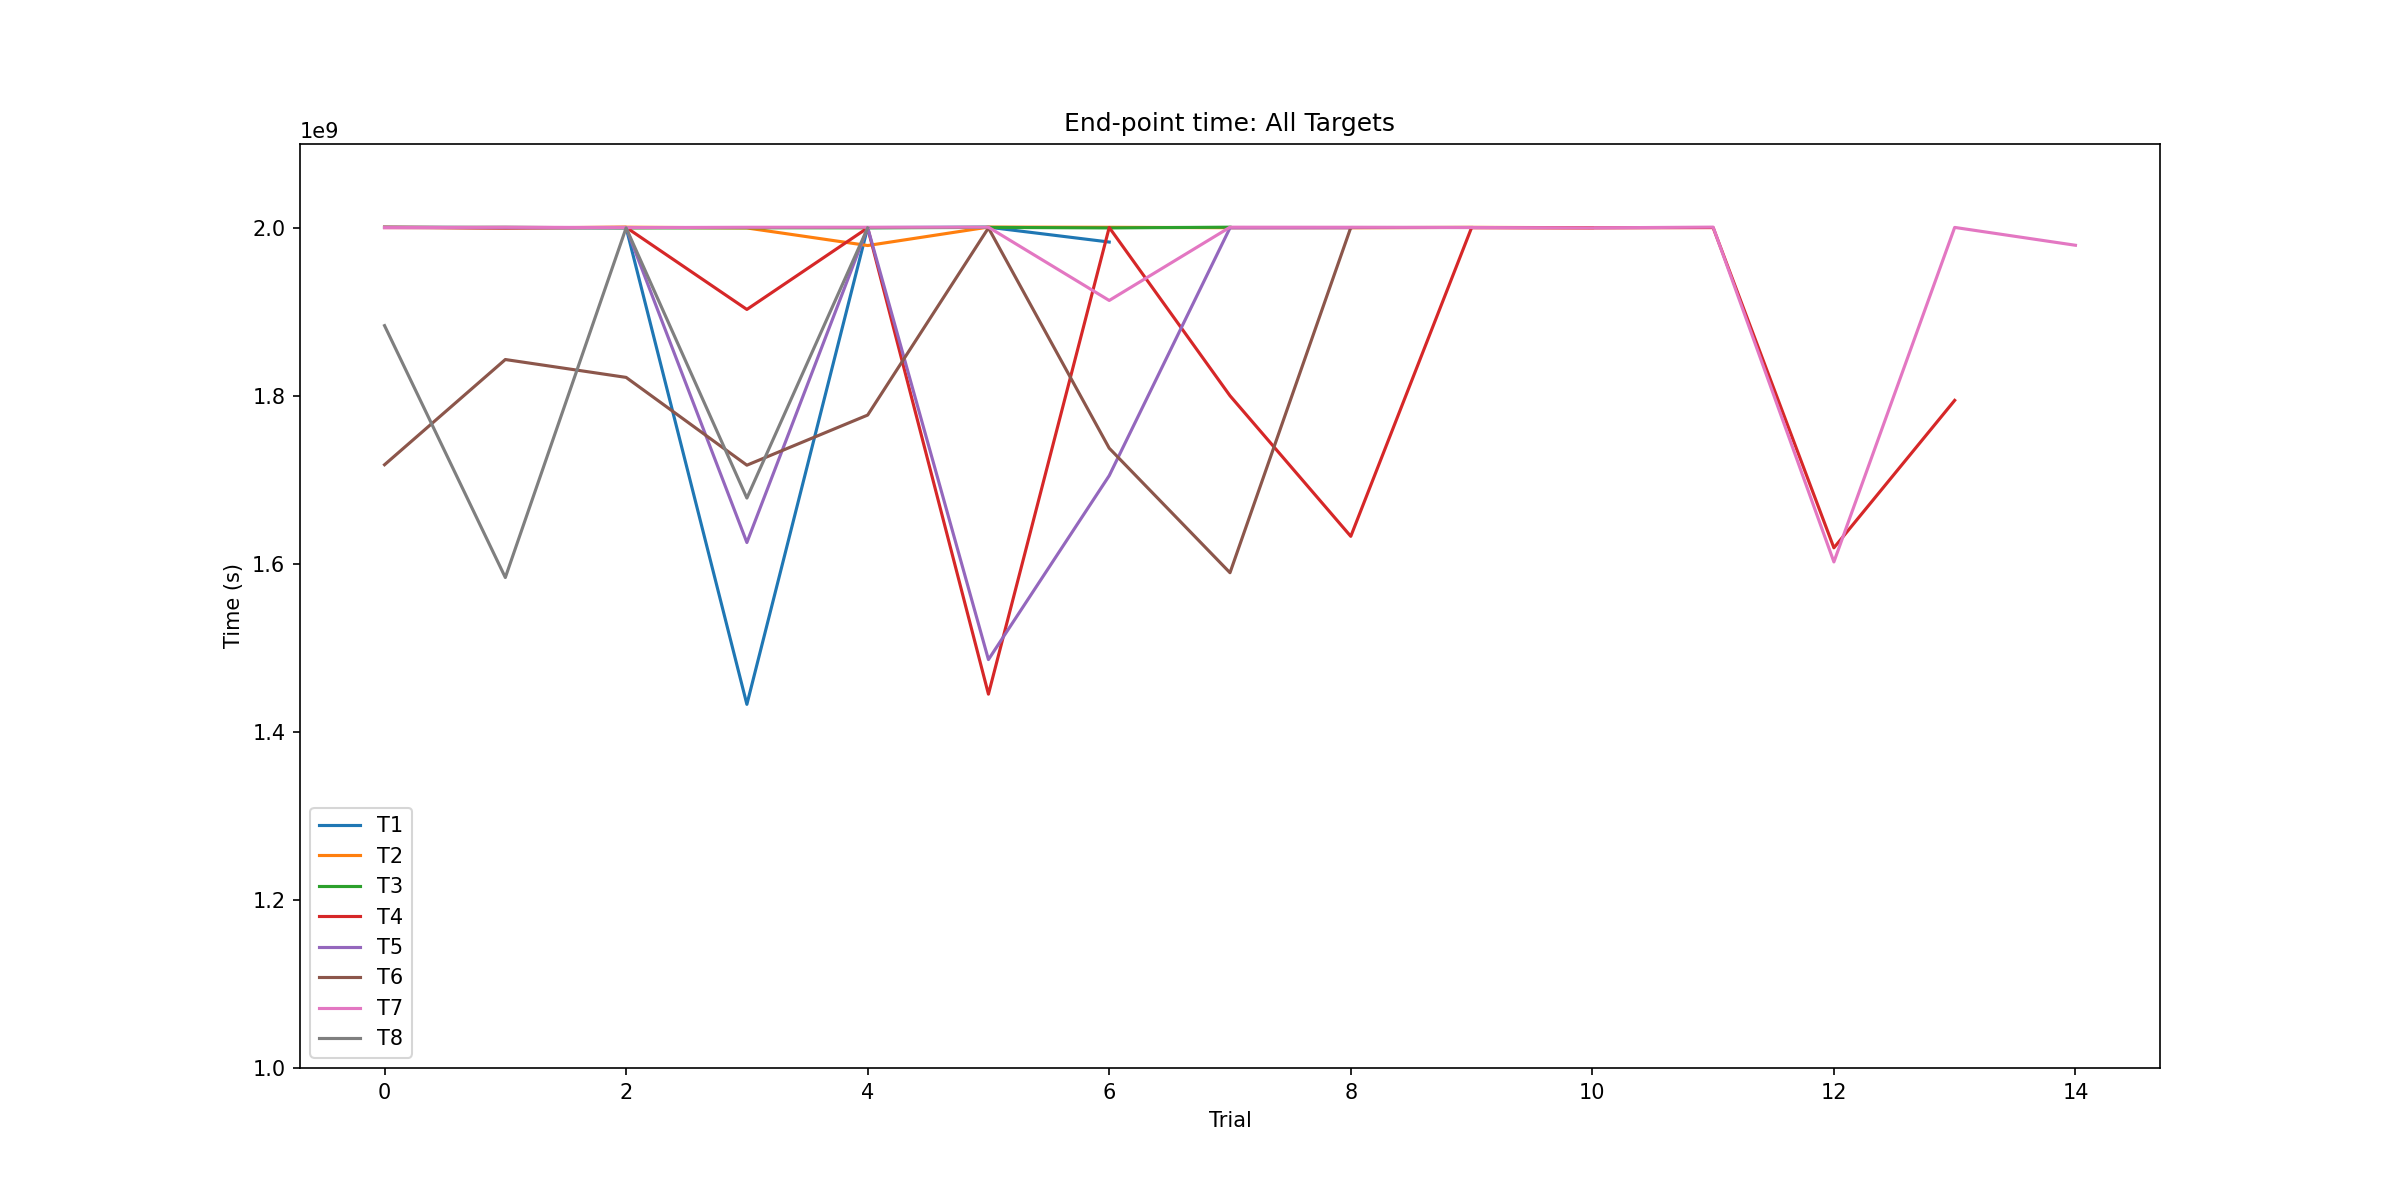
\includegraphics[width=\linewidth]{sujeto3/no_force/evolution_time}
		\caption{Sujeto 3, sin fuerza}
		\label{fig:figura1}
	\end{minipage}
	\hspace{0.5cm}
	\begin{minipage}[b]{0.5\linewidth}
		\centering
		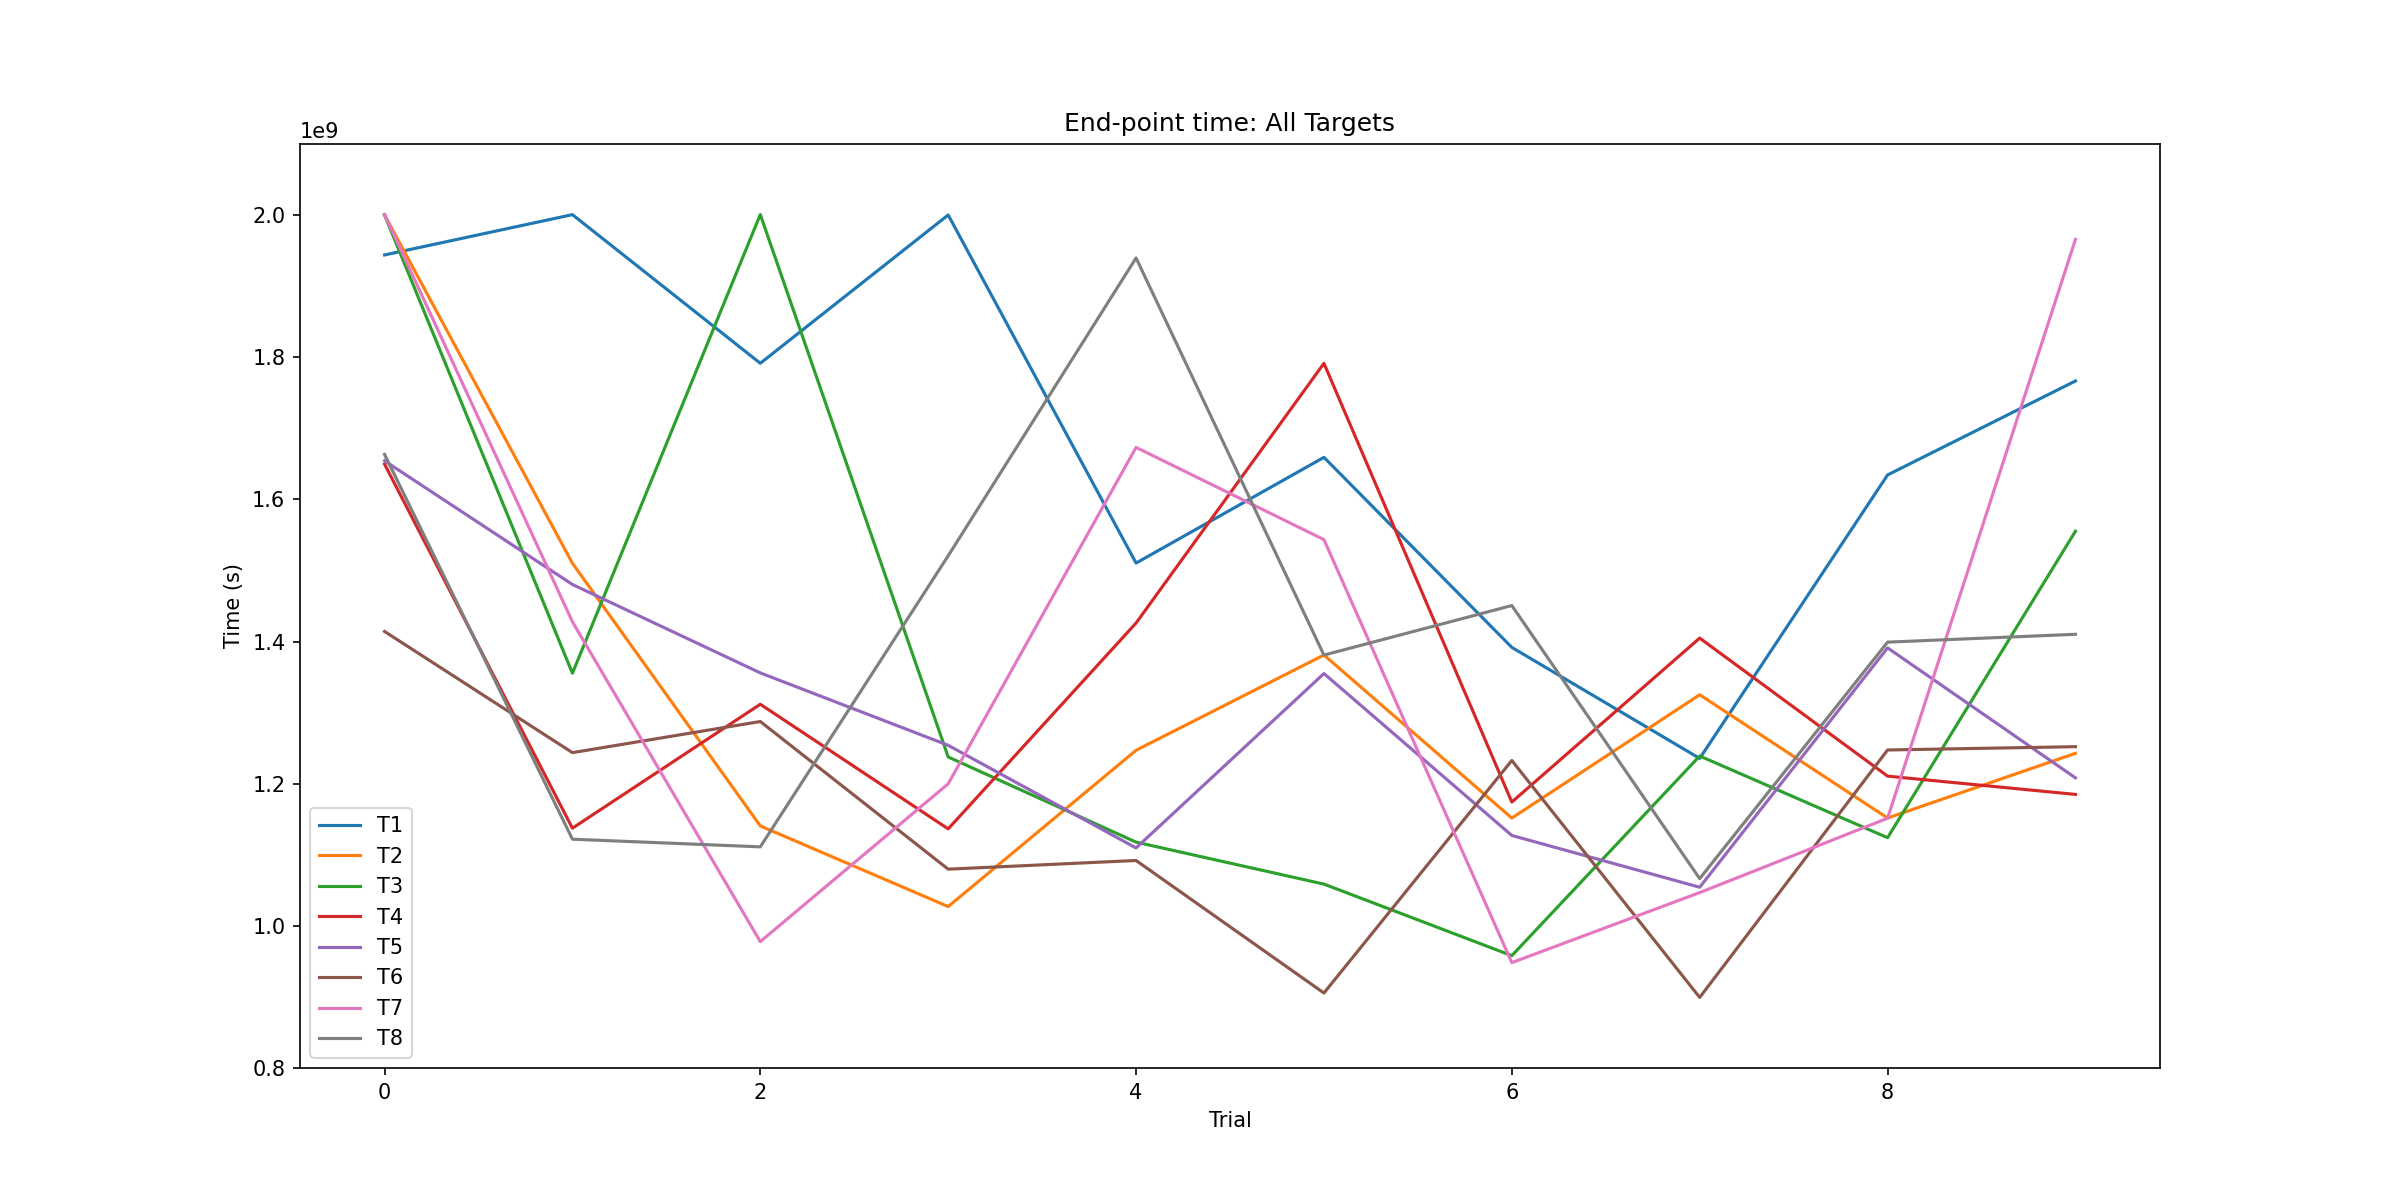
\includegraphics[width=\linewidth]{sujeto4/no_force/evolution_time}
		\caption{Sujeto 4, sin fuerza}
		\label{fig:figura2}
	\end{minipage}
\end{figure}
\begin{figure}[h]
	\begin{minipage}[b]{0.5\linewidth}
		\centering
		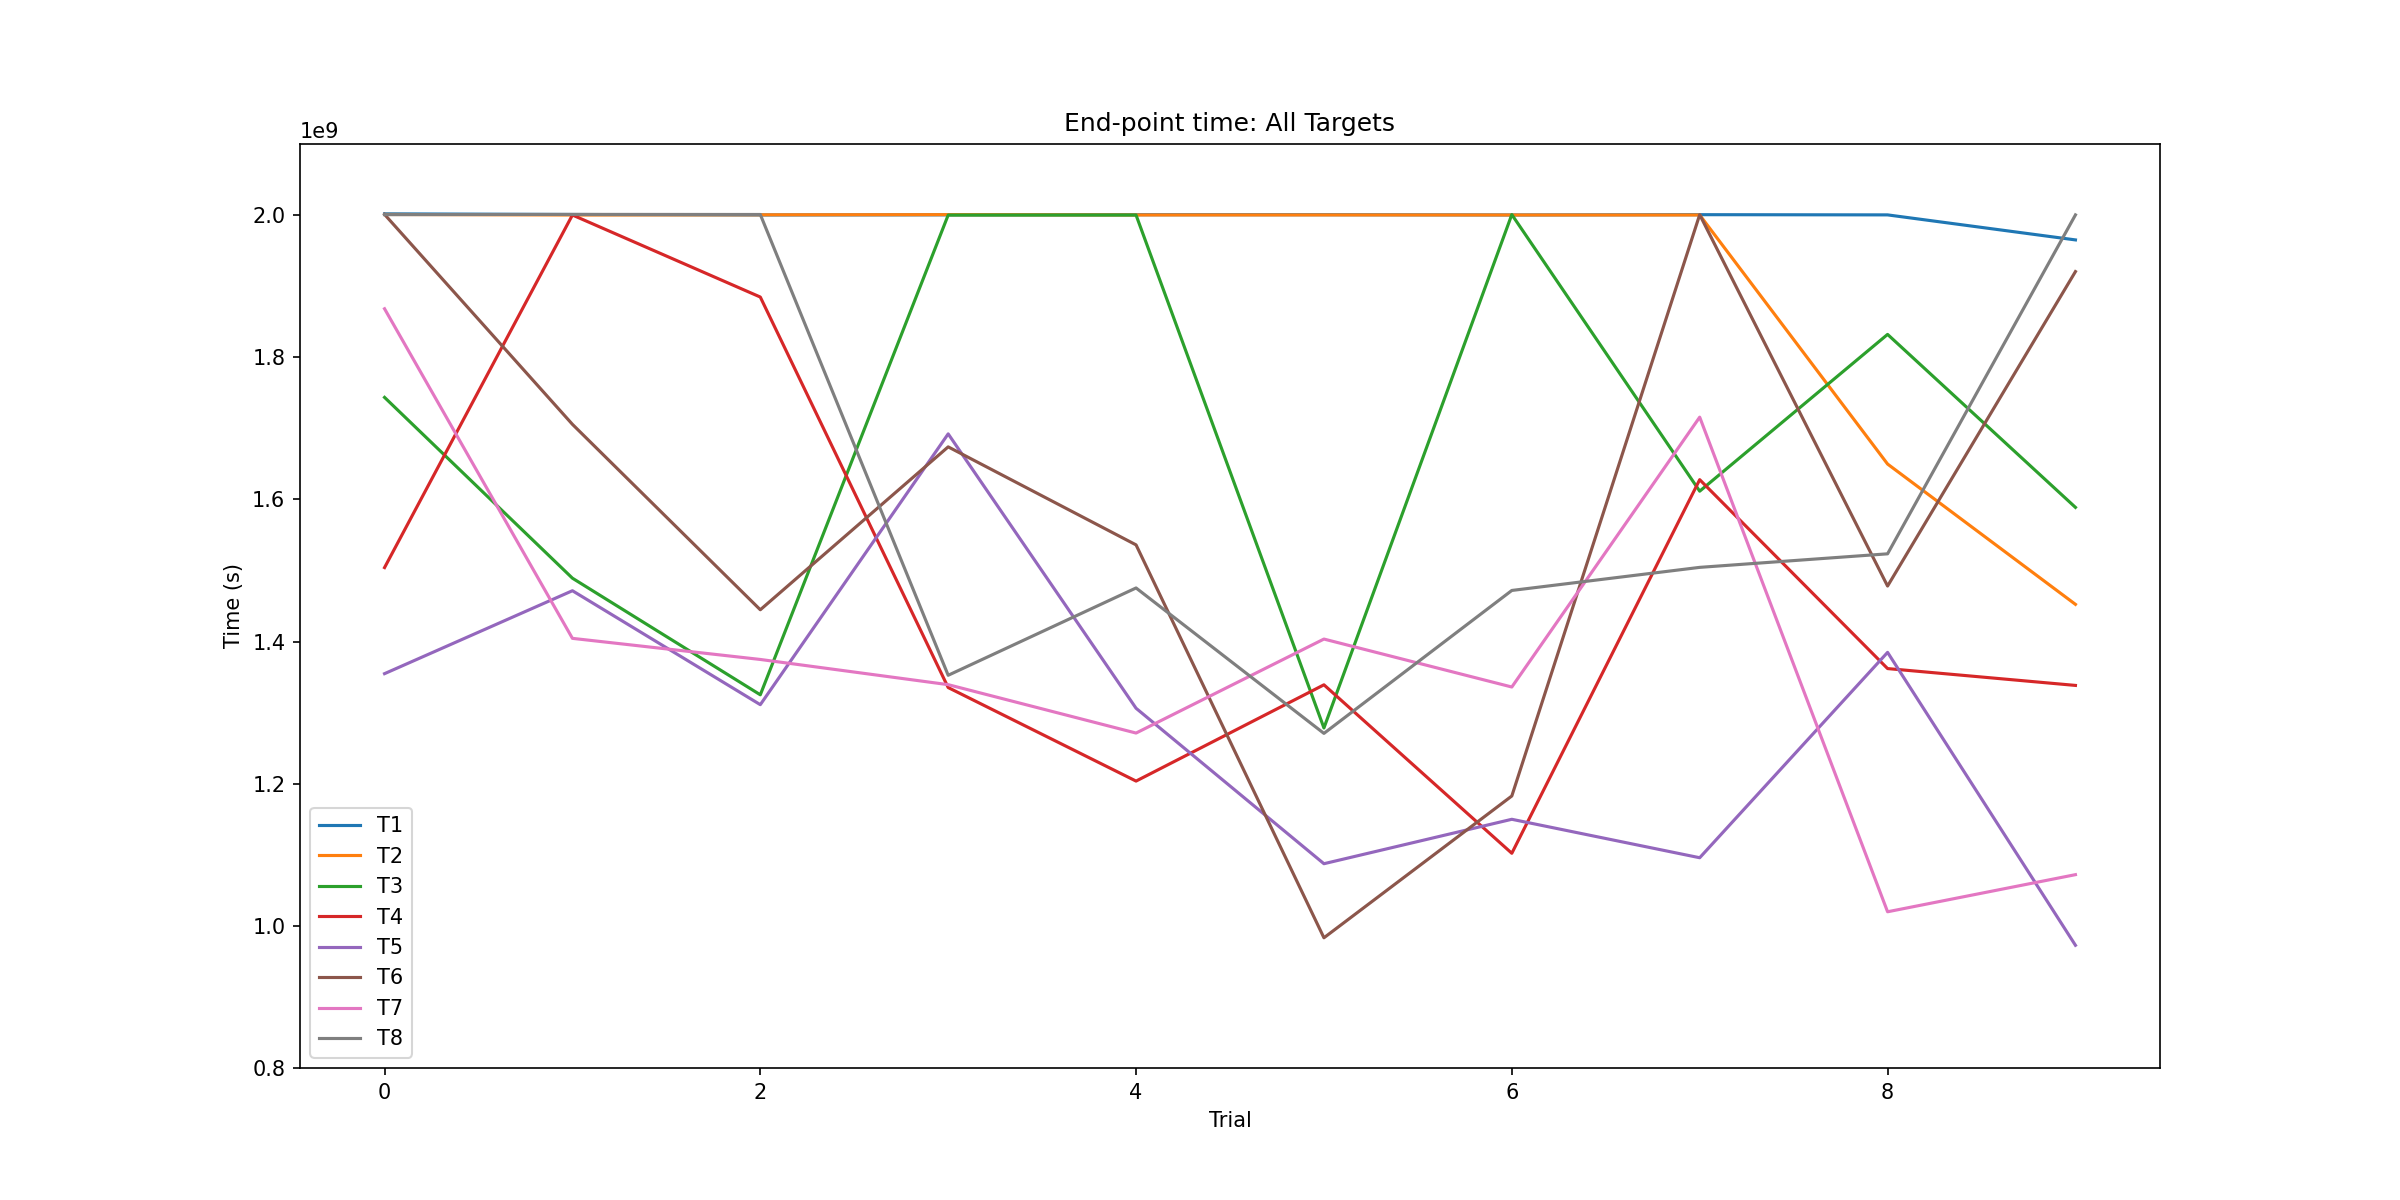
\includegraphics[width=\linewidth]{sujeto5/no_force/evolution_time}
		\caption{Sujeto 5, sin fuerza}
		\label{fig:figura1}
	\end{minipage}
\end{figure}

\subsubsection{Con fuerza}

Esta fase del experimento trataba de aprender a controlar y corregir la fuerza que aplicábamos al dispositivo Touch.

Estudiando las trayectorias de los movimientos podemos ver que hay una gran diferencia entre los sujetos de mayor edad y los de menor. Las trayectorias de los sujetos 1,2,4 están muy definidas, teniendo los primeros movimientos en cada punto trayectorias más largas (las trayectorias rojas más claras) y luego siendo cada vez líneas más rectas (las negras). Las trayectorias de los sujetos 3 y 5, sin embargo, son bastante más difusas, con especial mención del sujeto 5, que en todo momento se deja llevar por la fuerza.

Sujetos más jóvenes:
\\

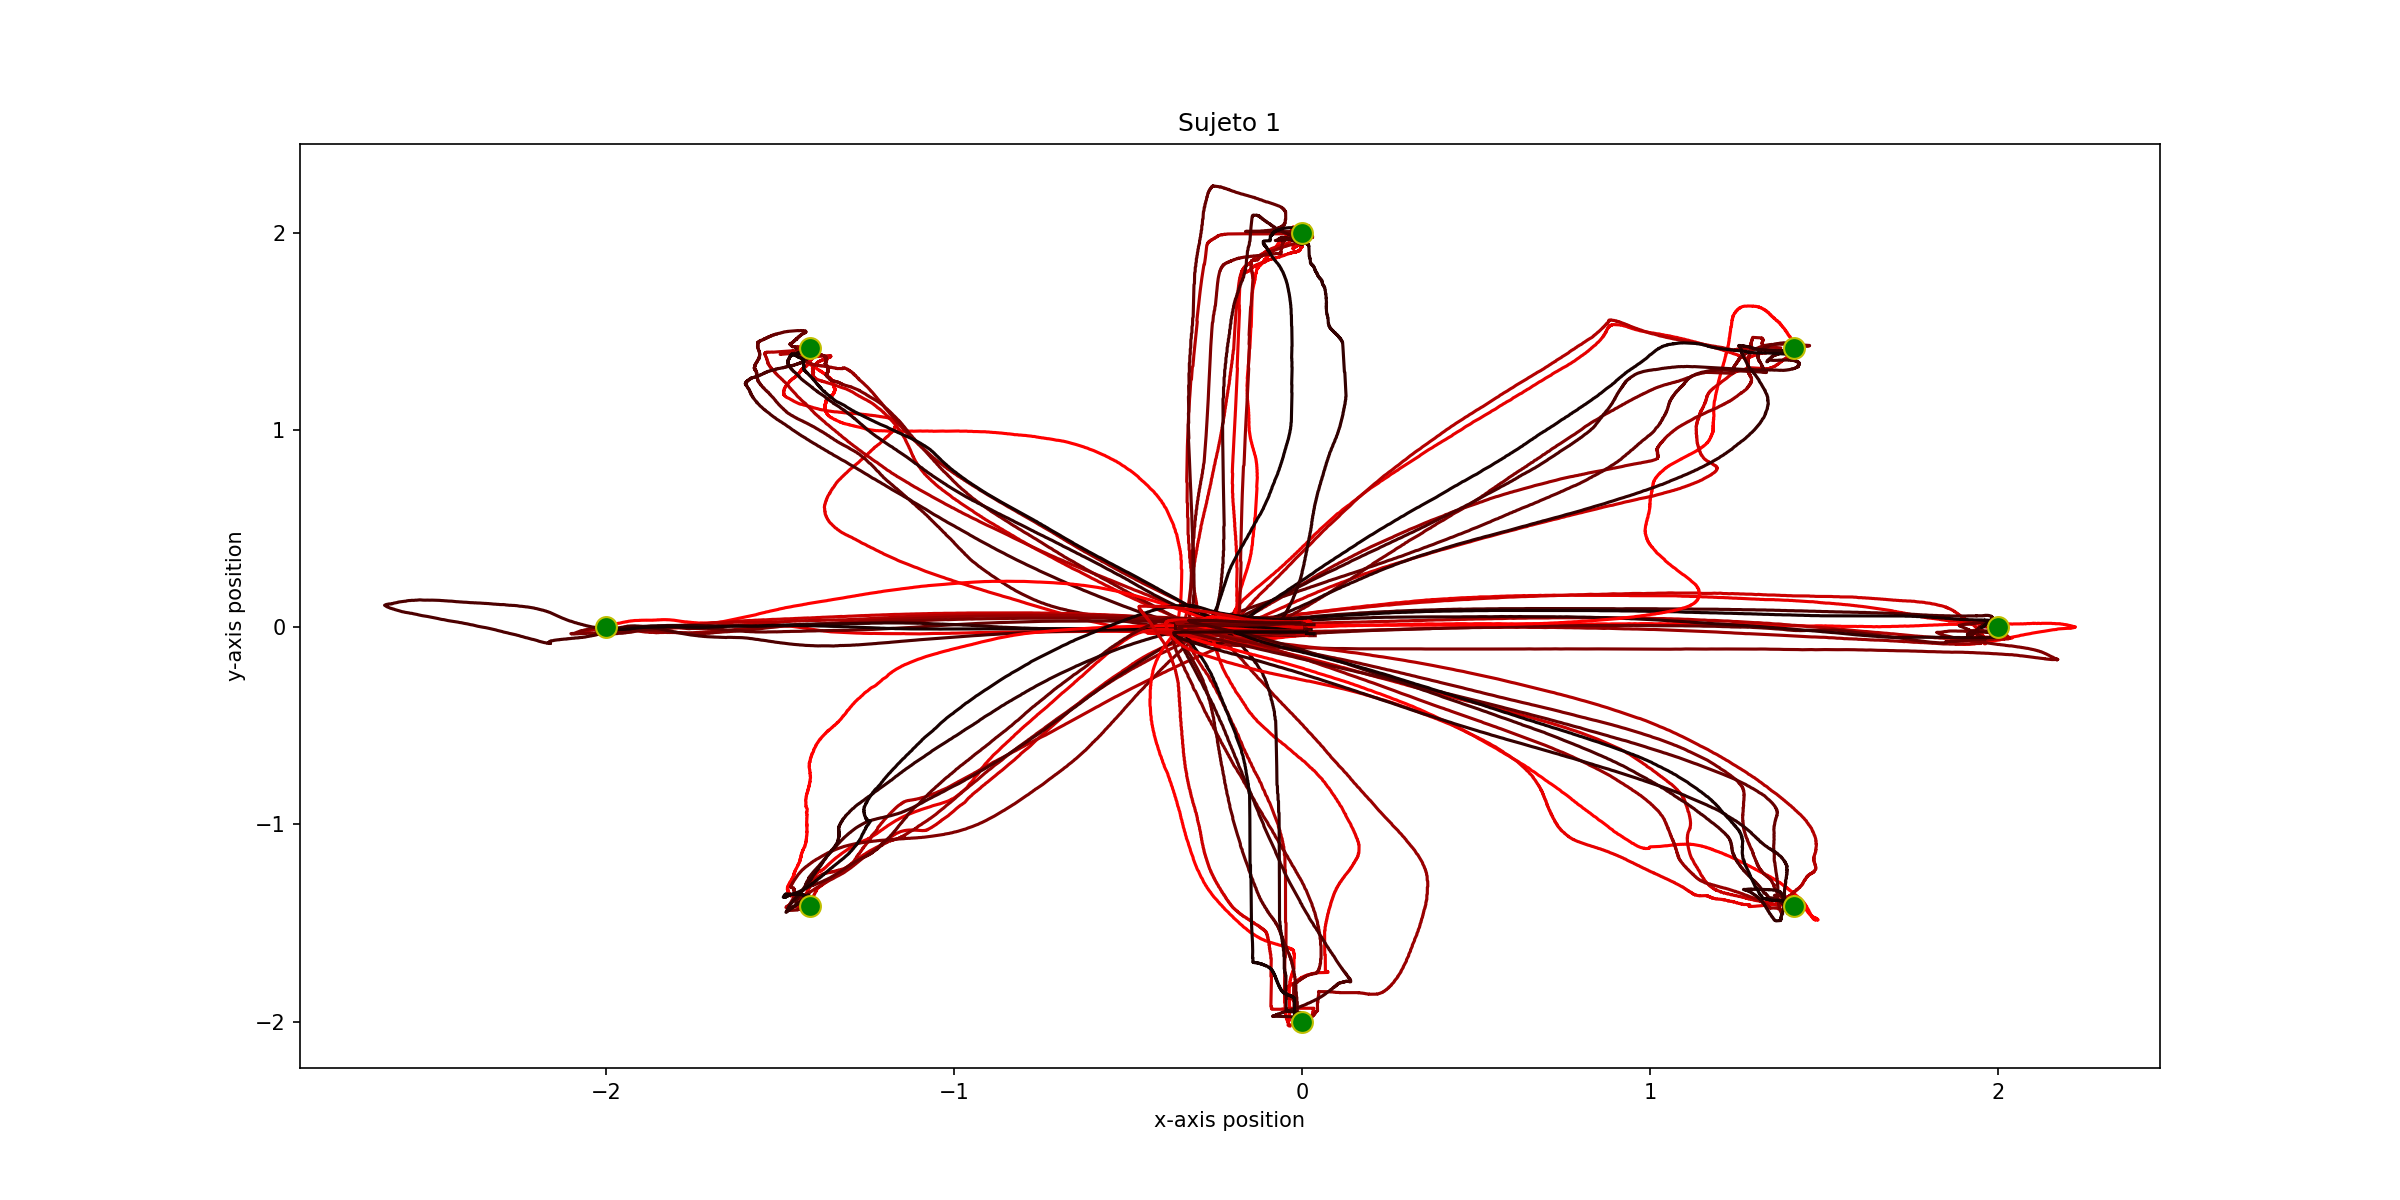
\includegraphics[scale=0.2]{sujeto1/force/trayectorias}
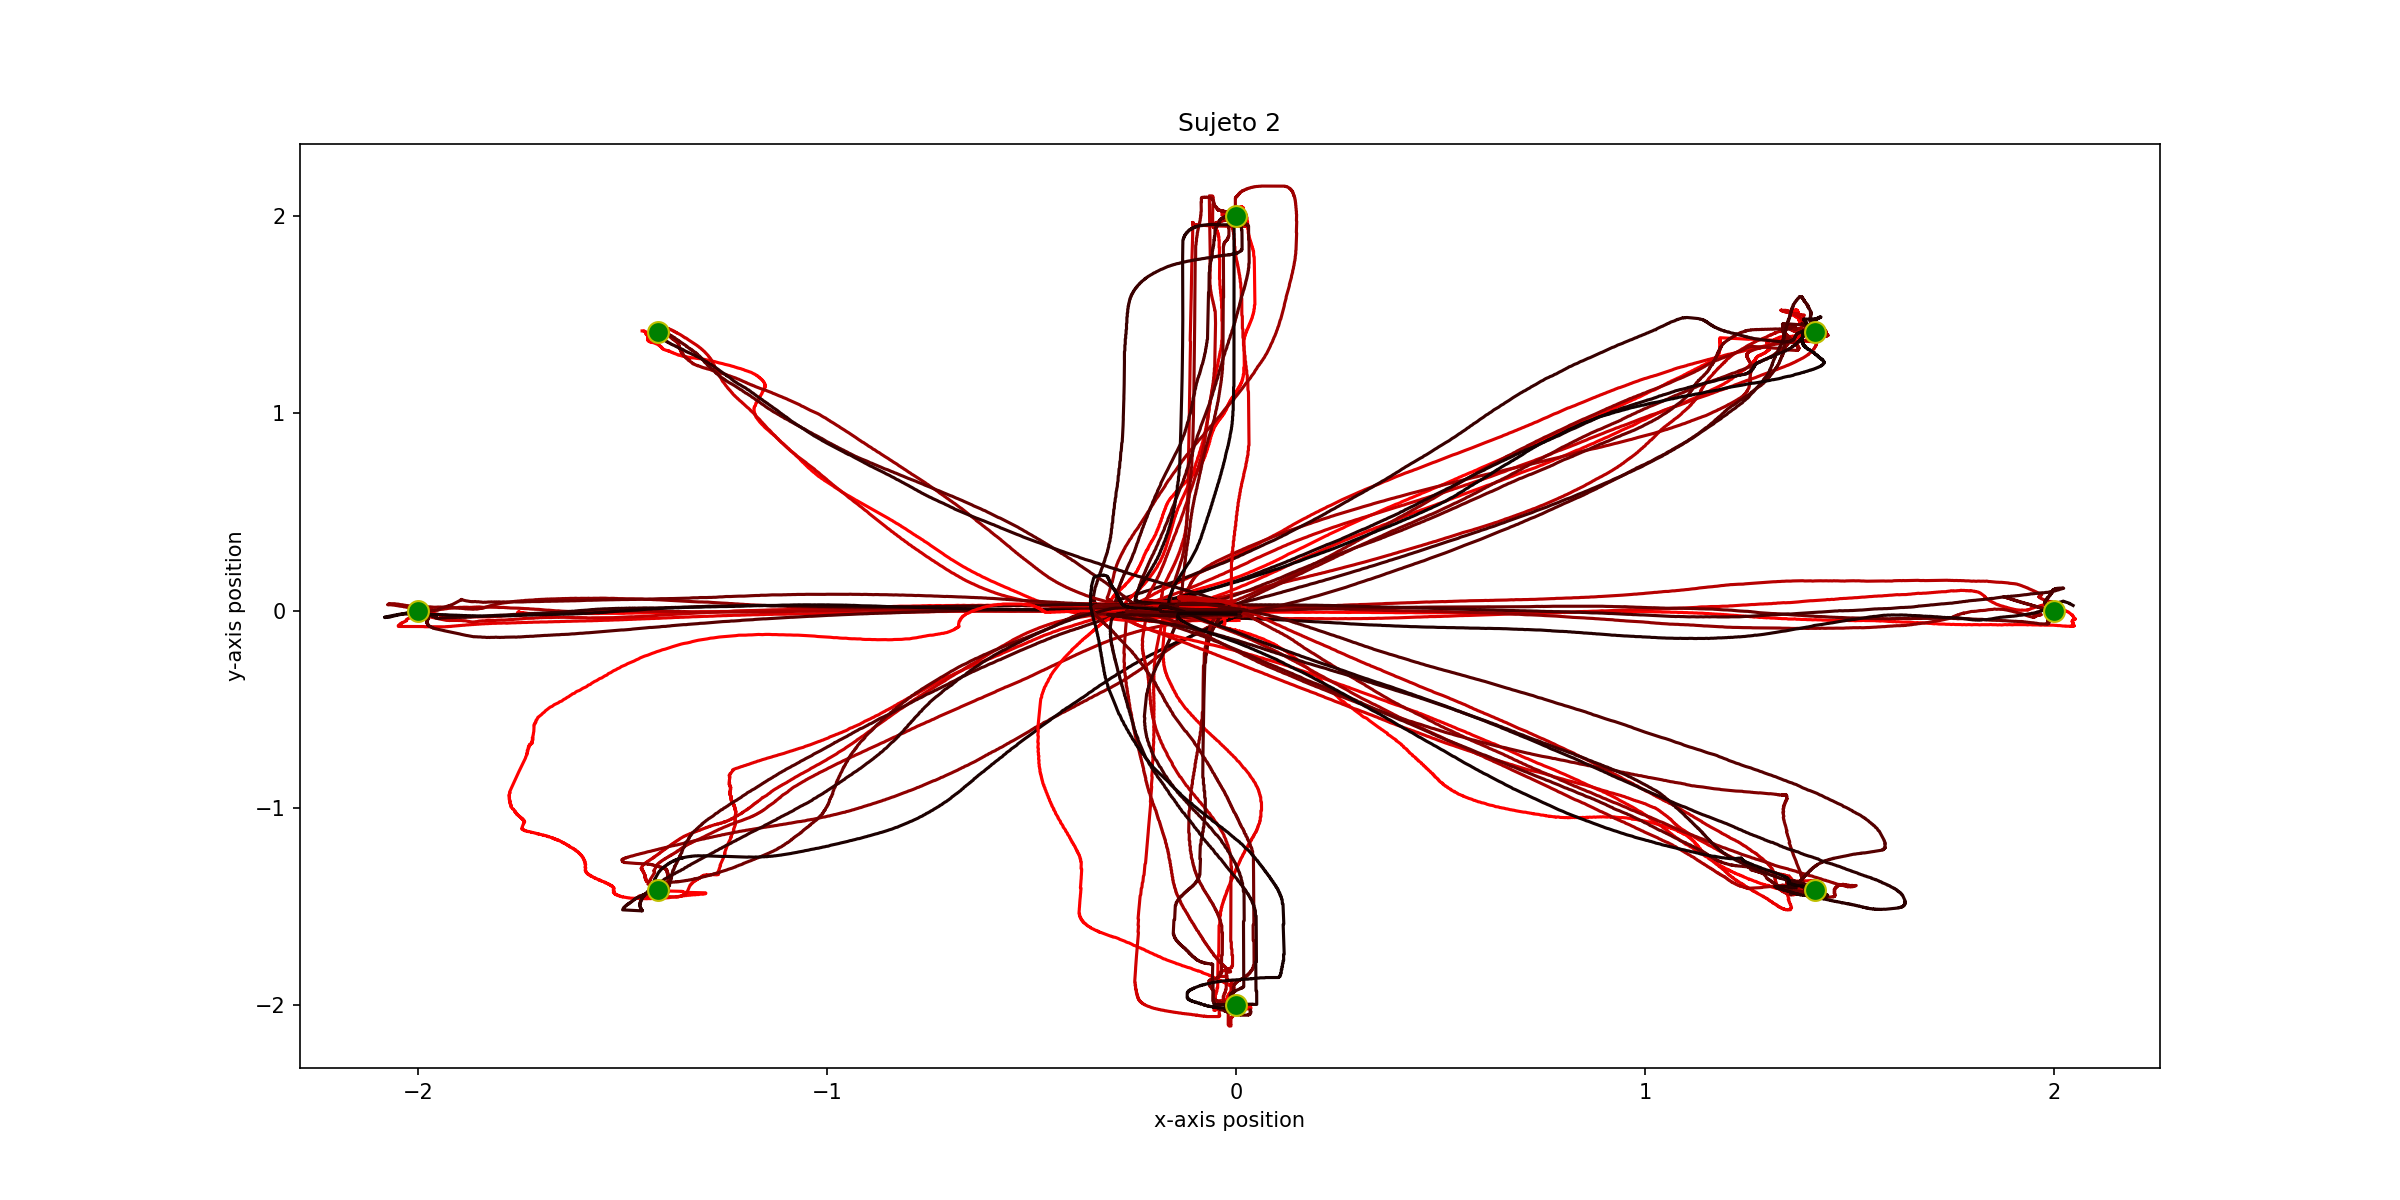
\includegraphics[scale=0.2]{sujeto2/force/trayectorias}
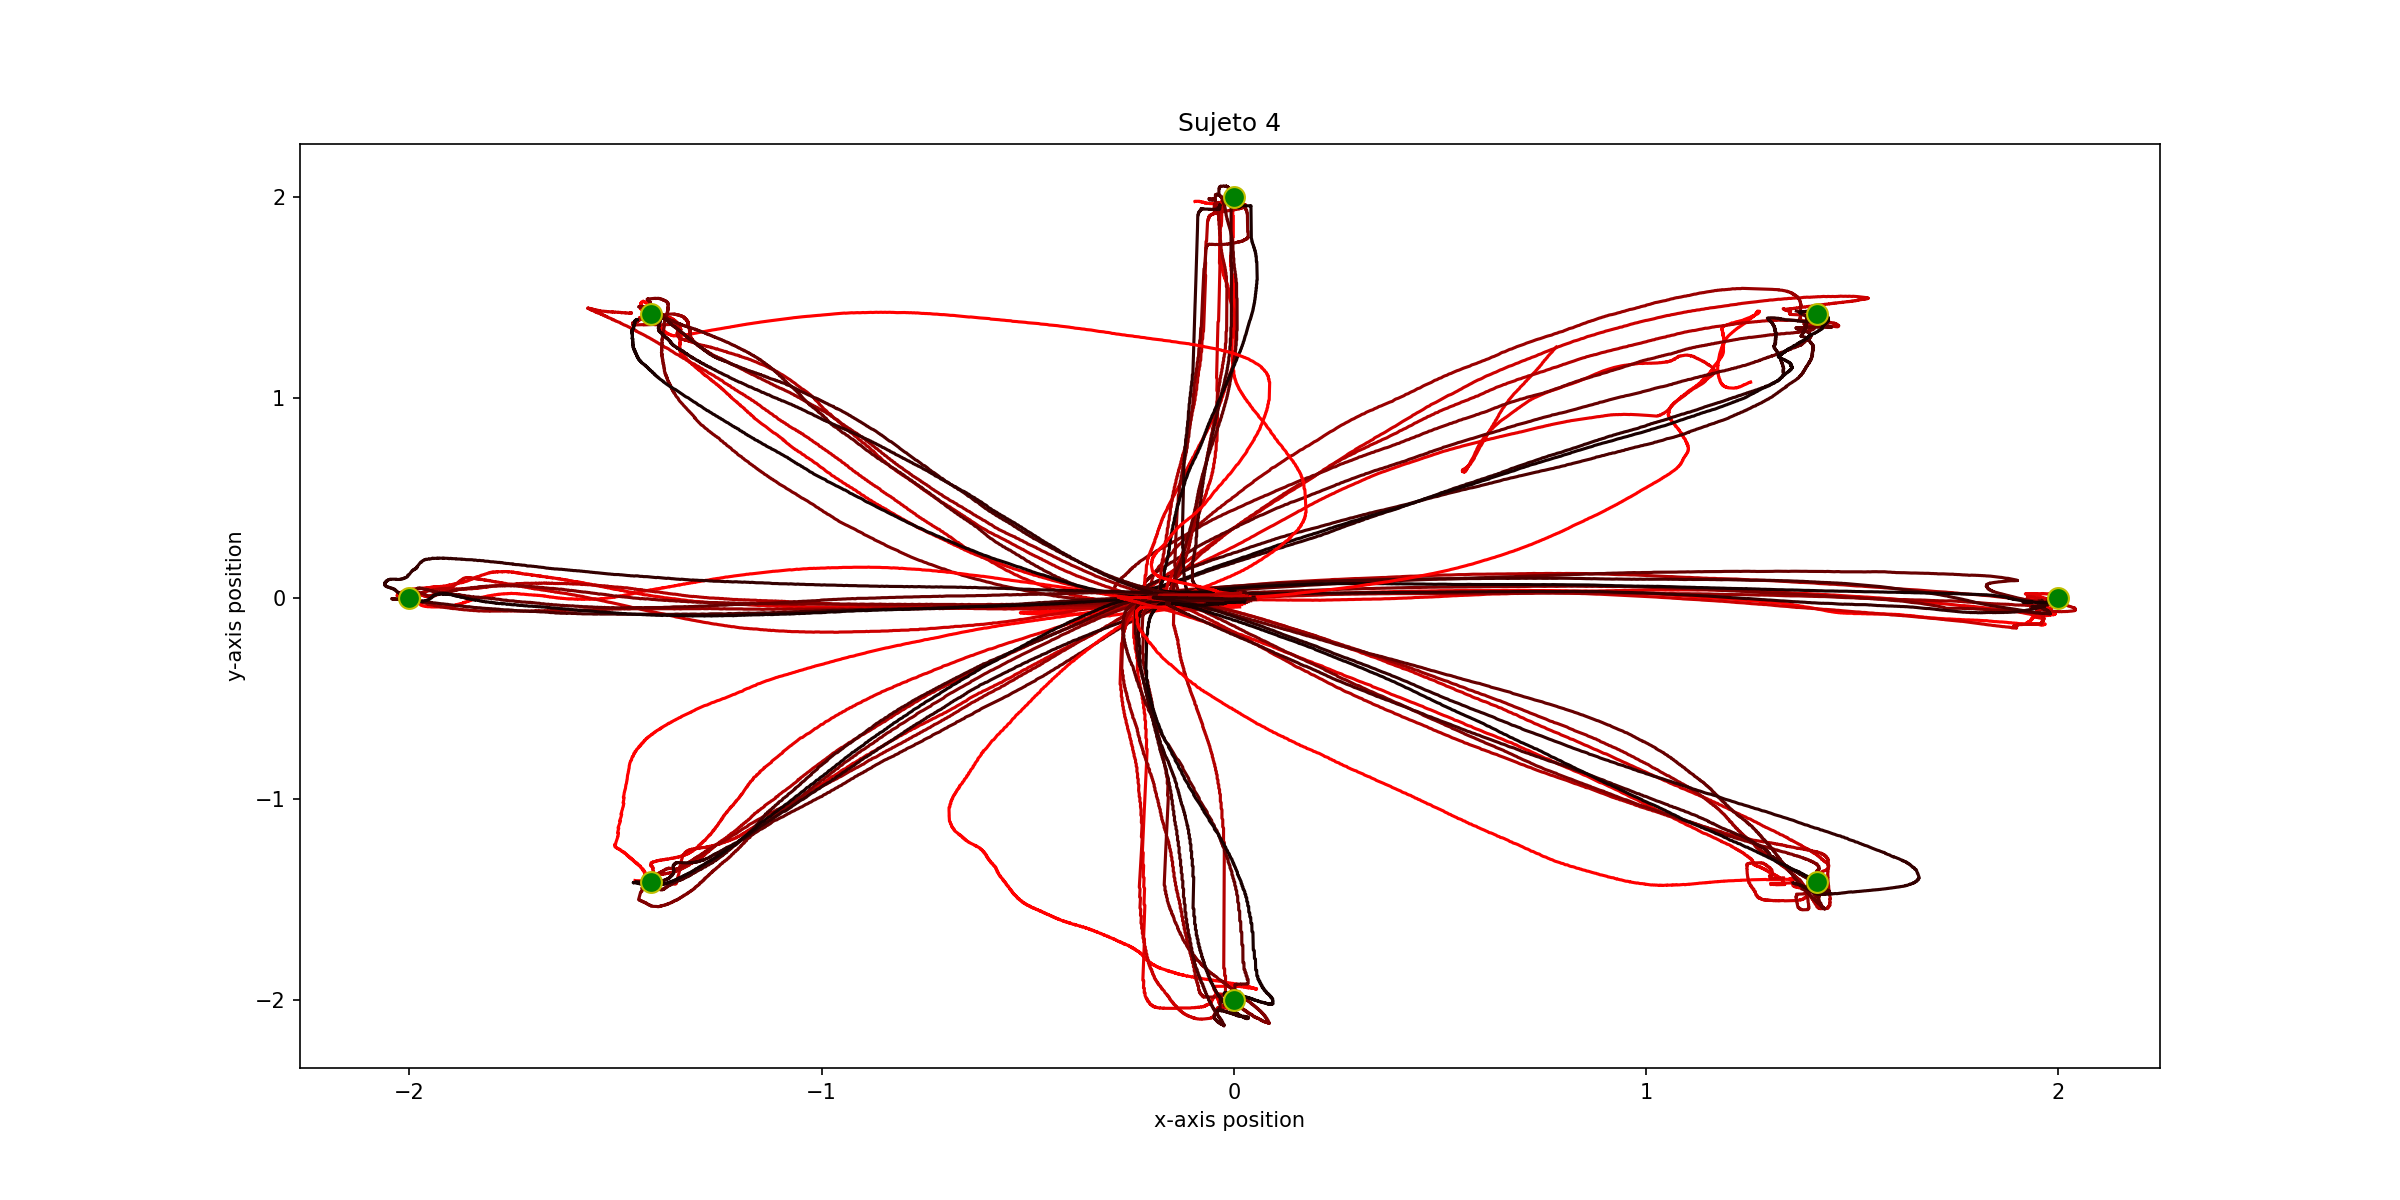
\includegraphics[scale=0.2]{sujeto4/force/trayectorias}

Sujetos mayores de 60 años:
\\
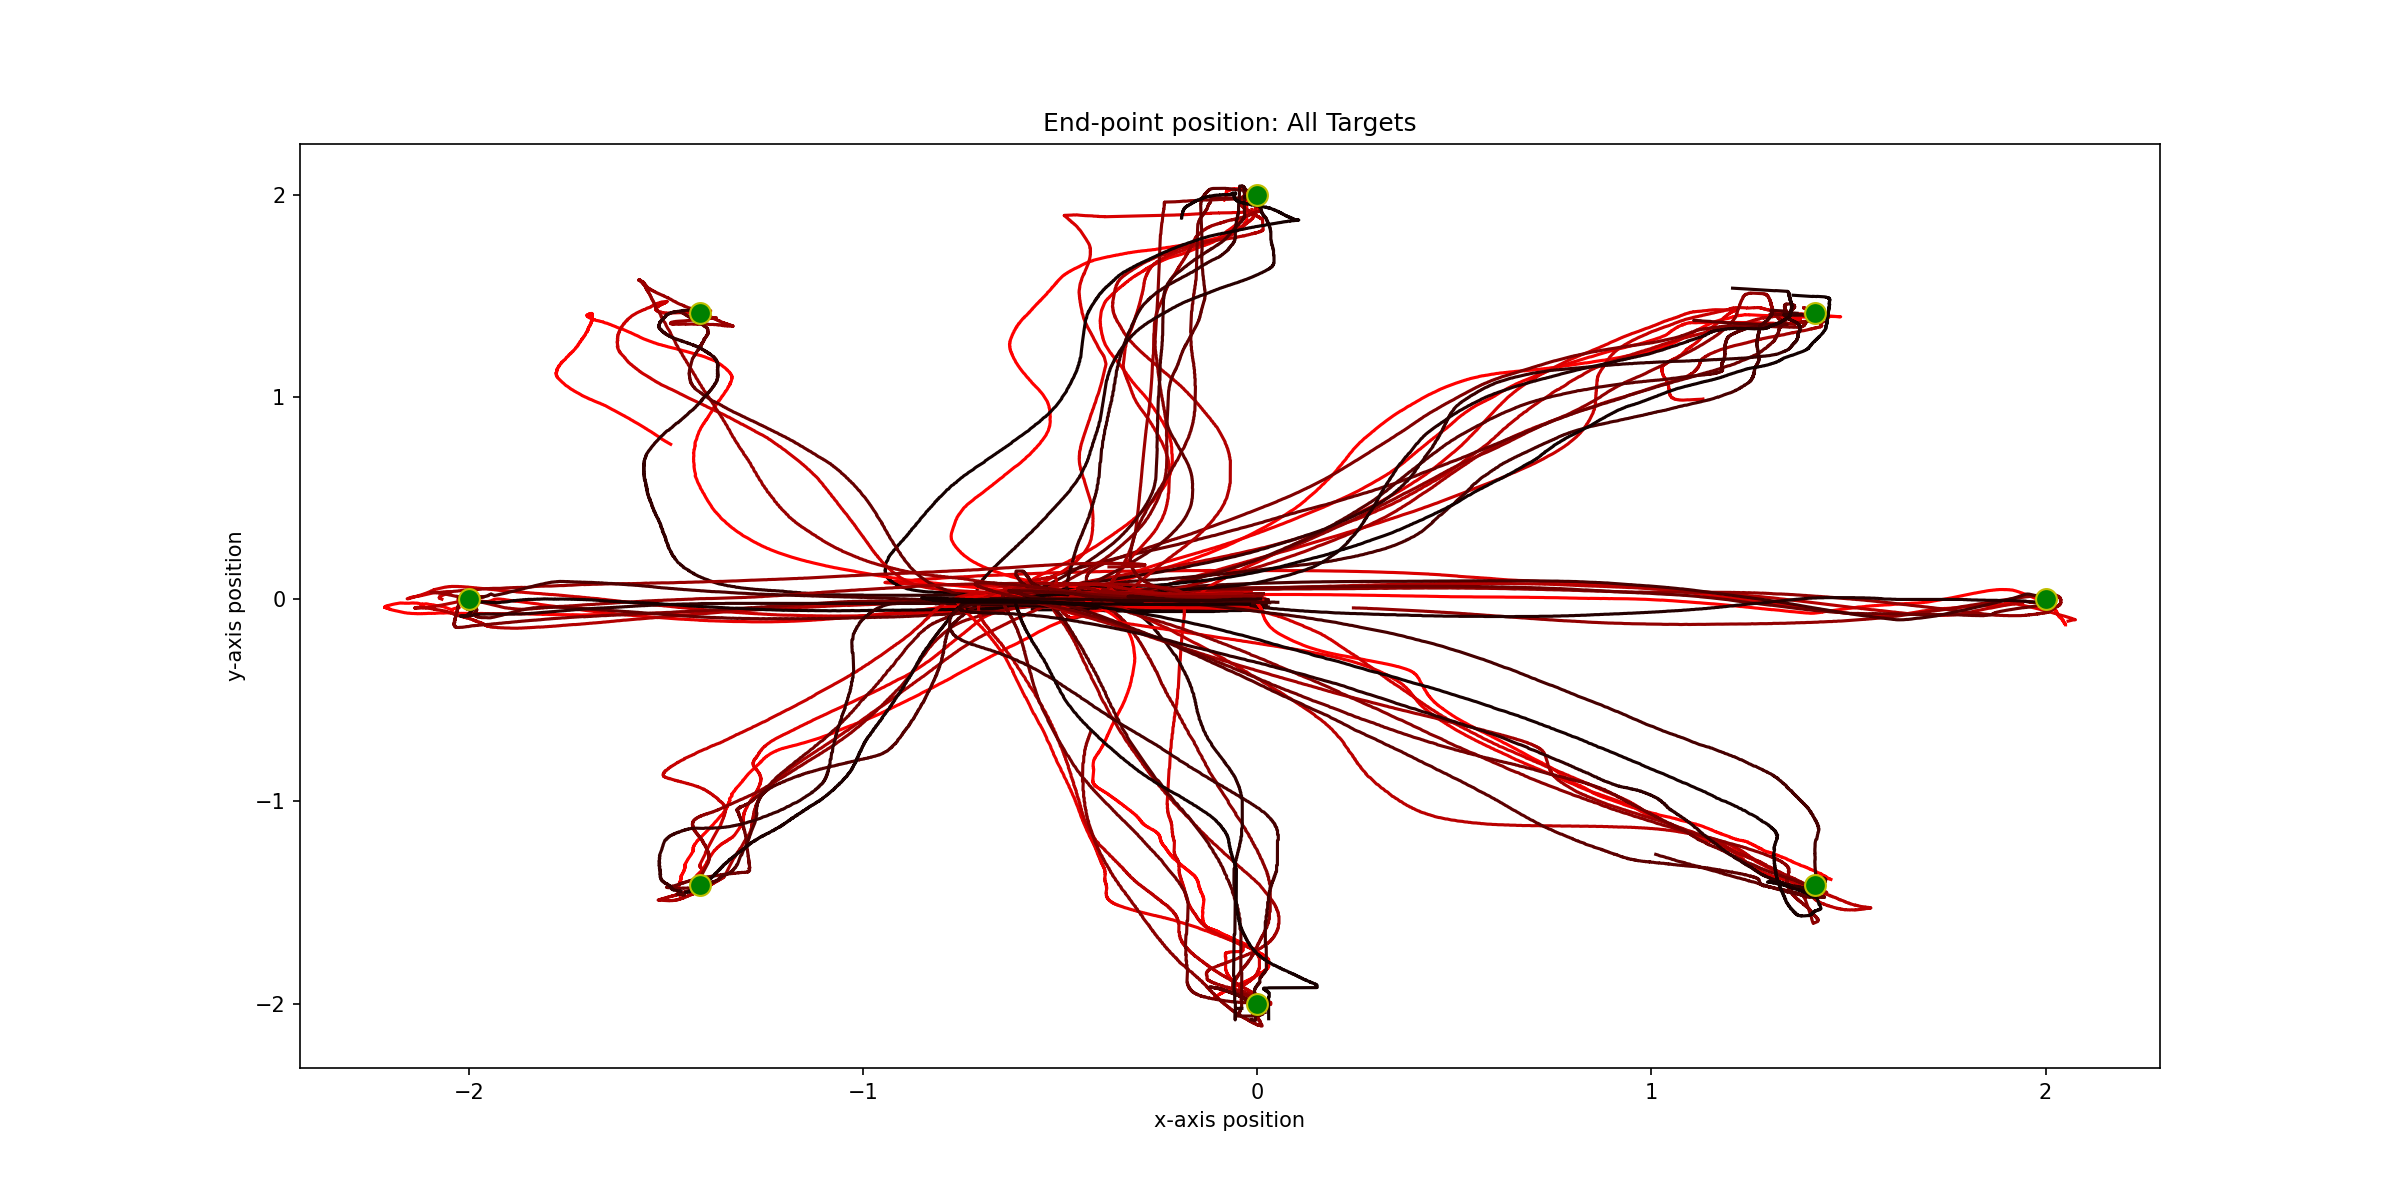
\includegraphics[scale=0.2]{sujeto3/force/trayectorias}
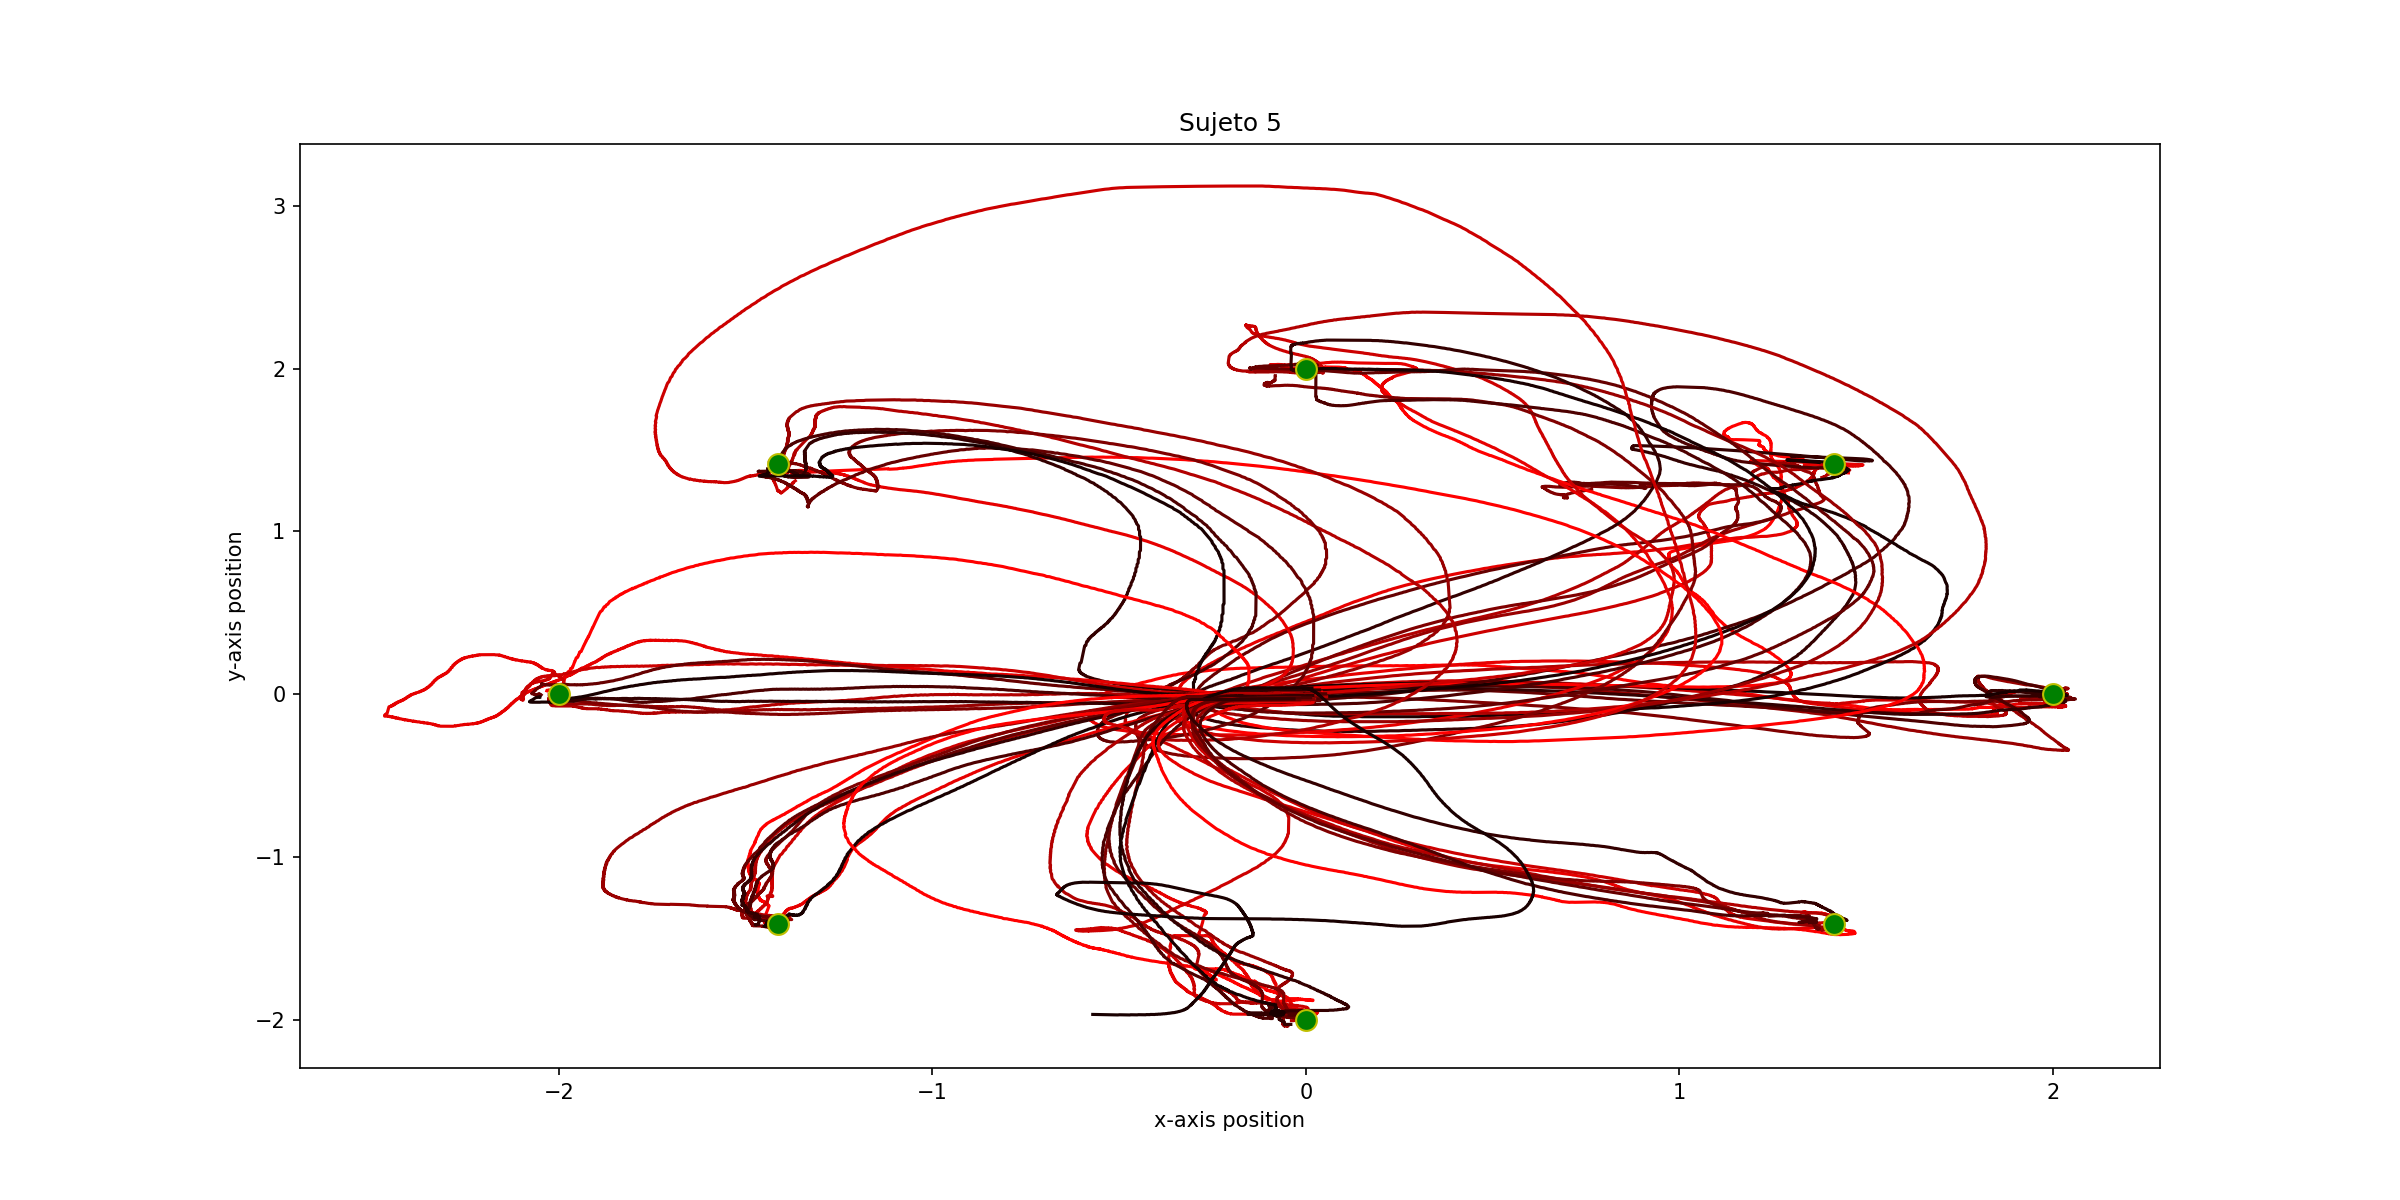
\includegraphics[scale=0.2]{sujeto5/force/trayectorias}

Si estudiamos sin embargo la distribución de puntos finales podemos observar que la precisión del sujeto 5 ha sido algo peor que la de los sujetos jóvenes, pero mejor que la del sujeto 3, concentrándose los errores en T2 y T7.

Sujetos jóvenes:
\\
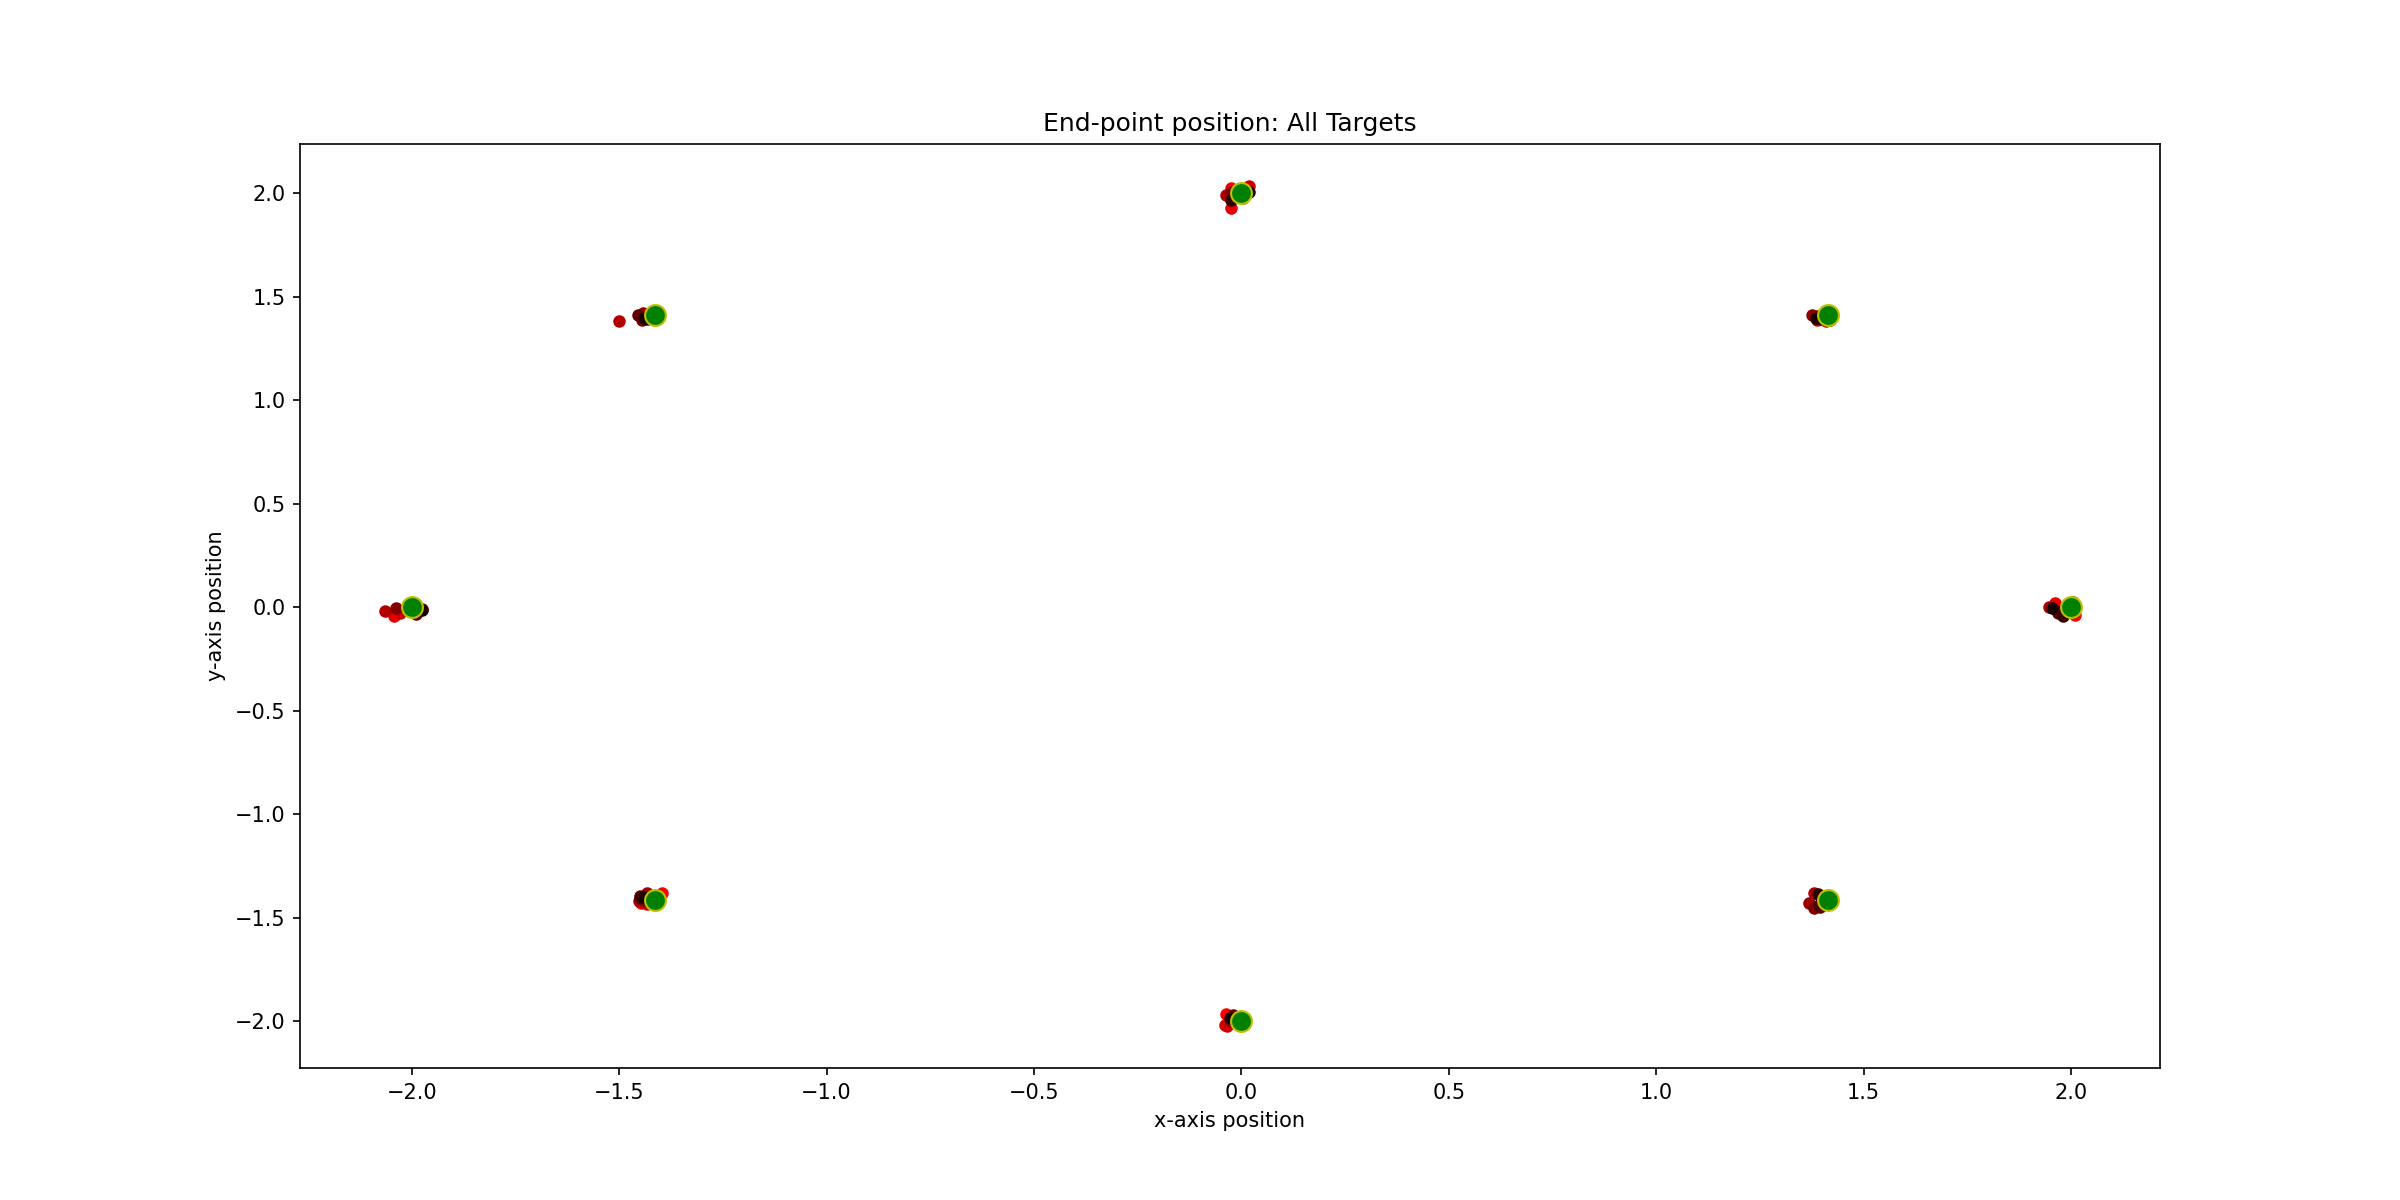
\includegraphics[scale=0.2]{sujeto1/force/trayectorias_puntos}
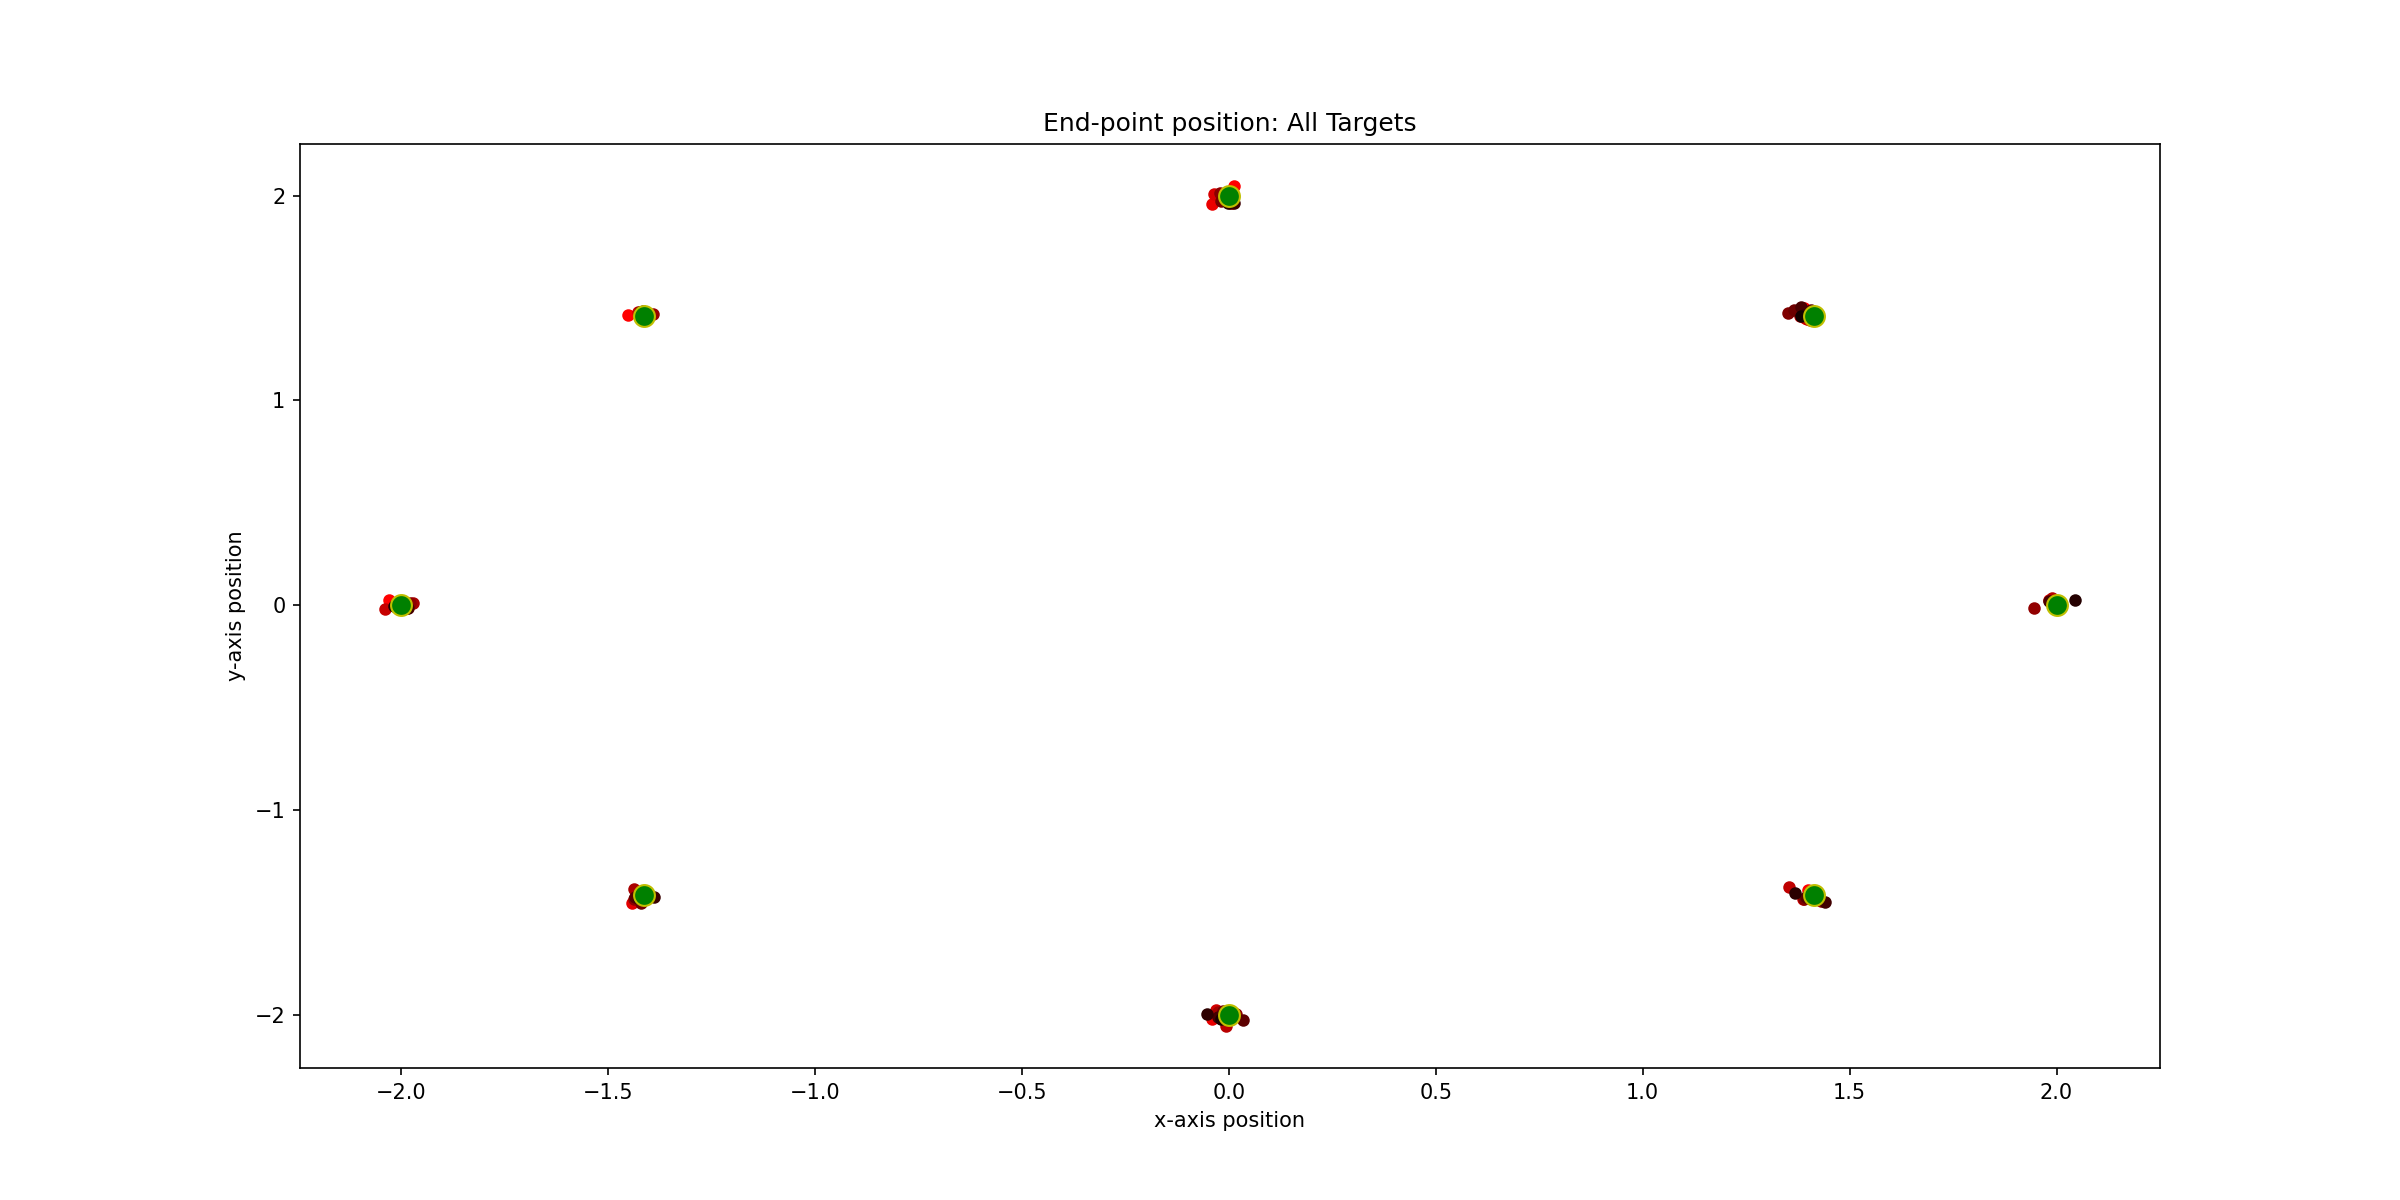
\includegraphics[scale=0.2]{sujeto2/force/trayectorias_puntos}
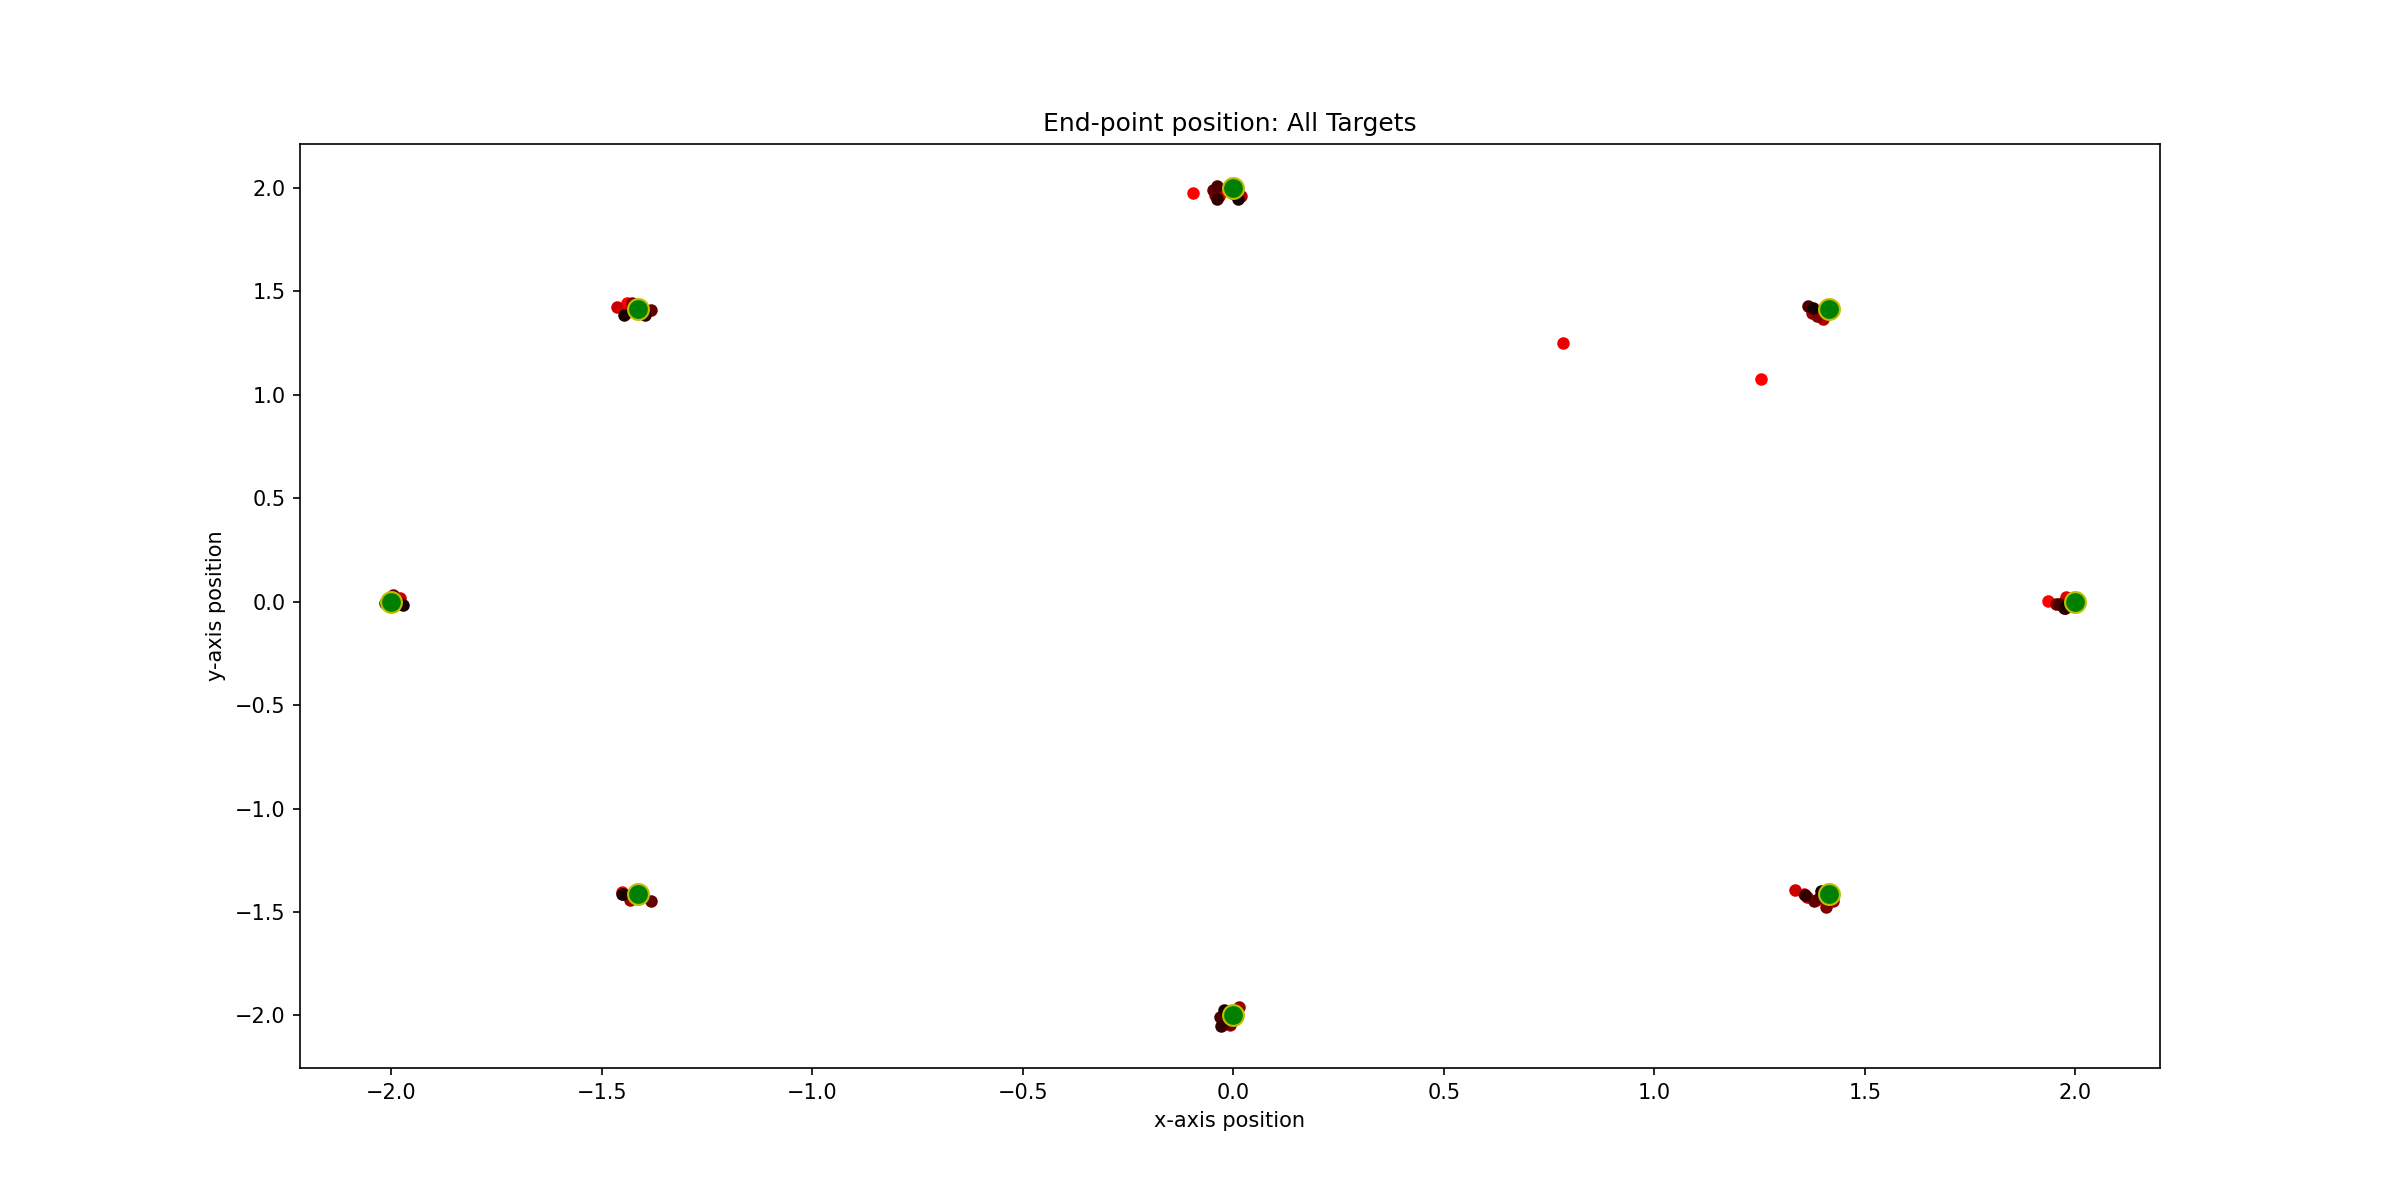
\includegraphics[scale=0.2]{sujeto4/force/trayectorias_puntos}

Sujetos mayores de 60 años:
\\
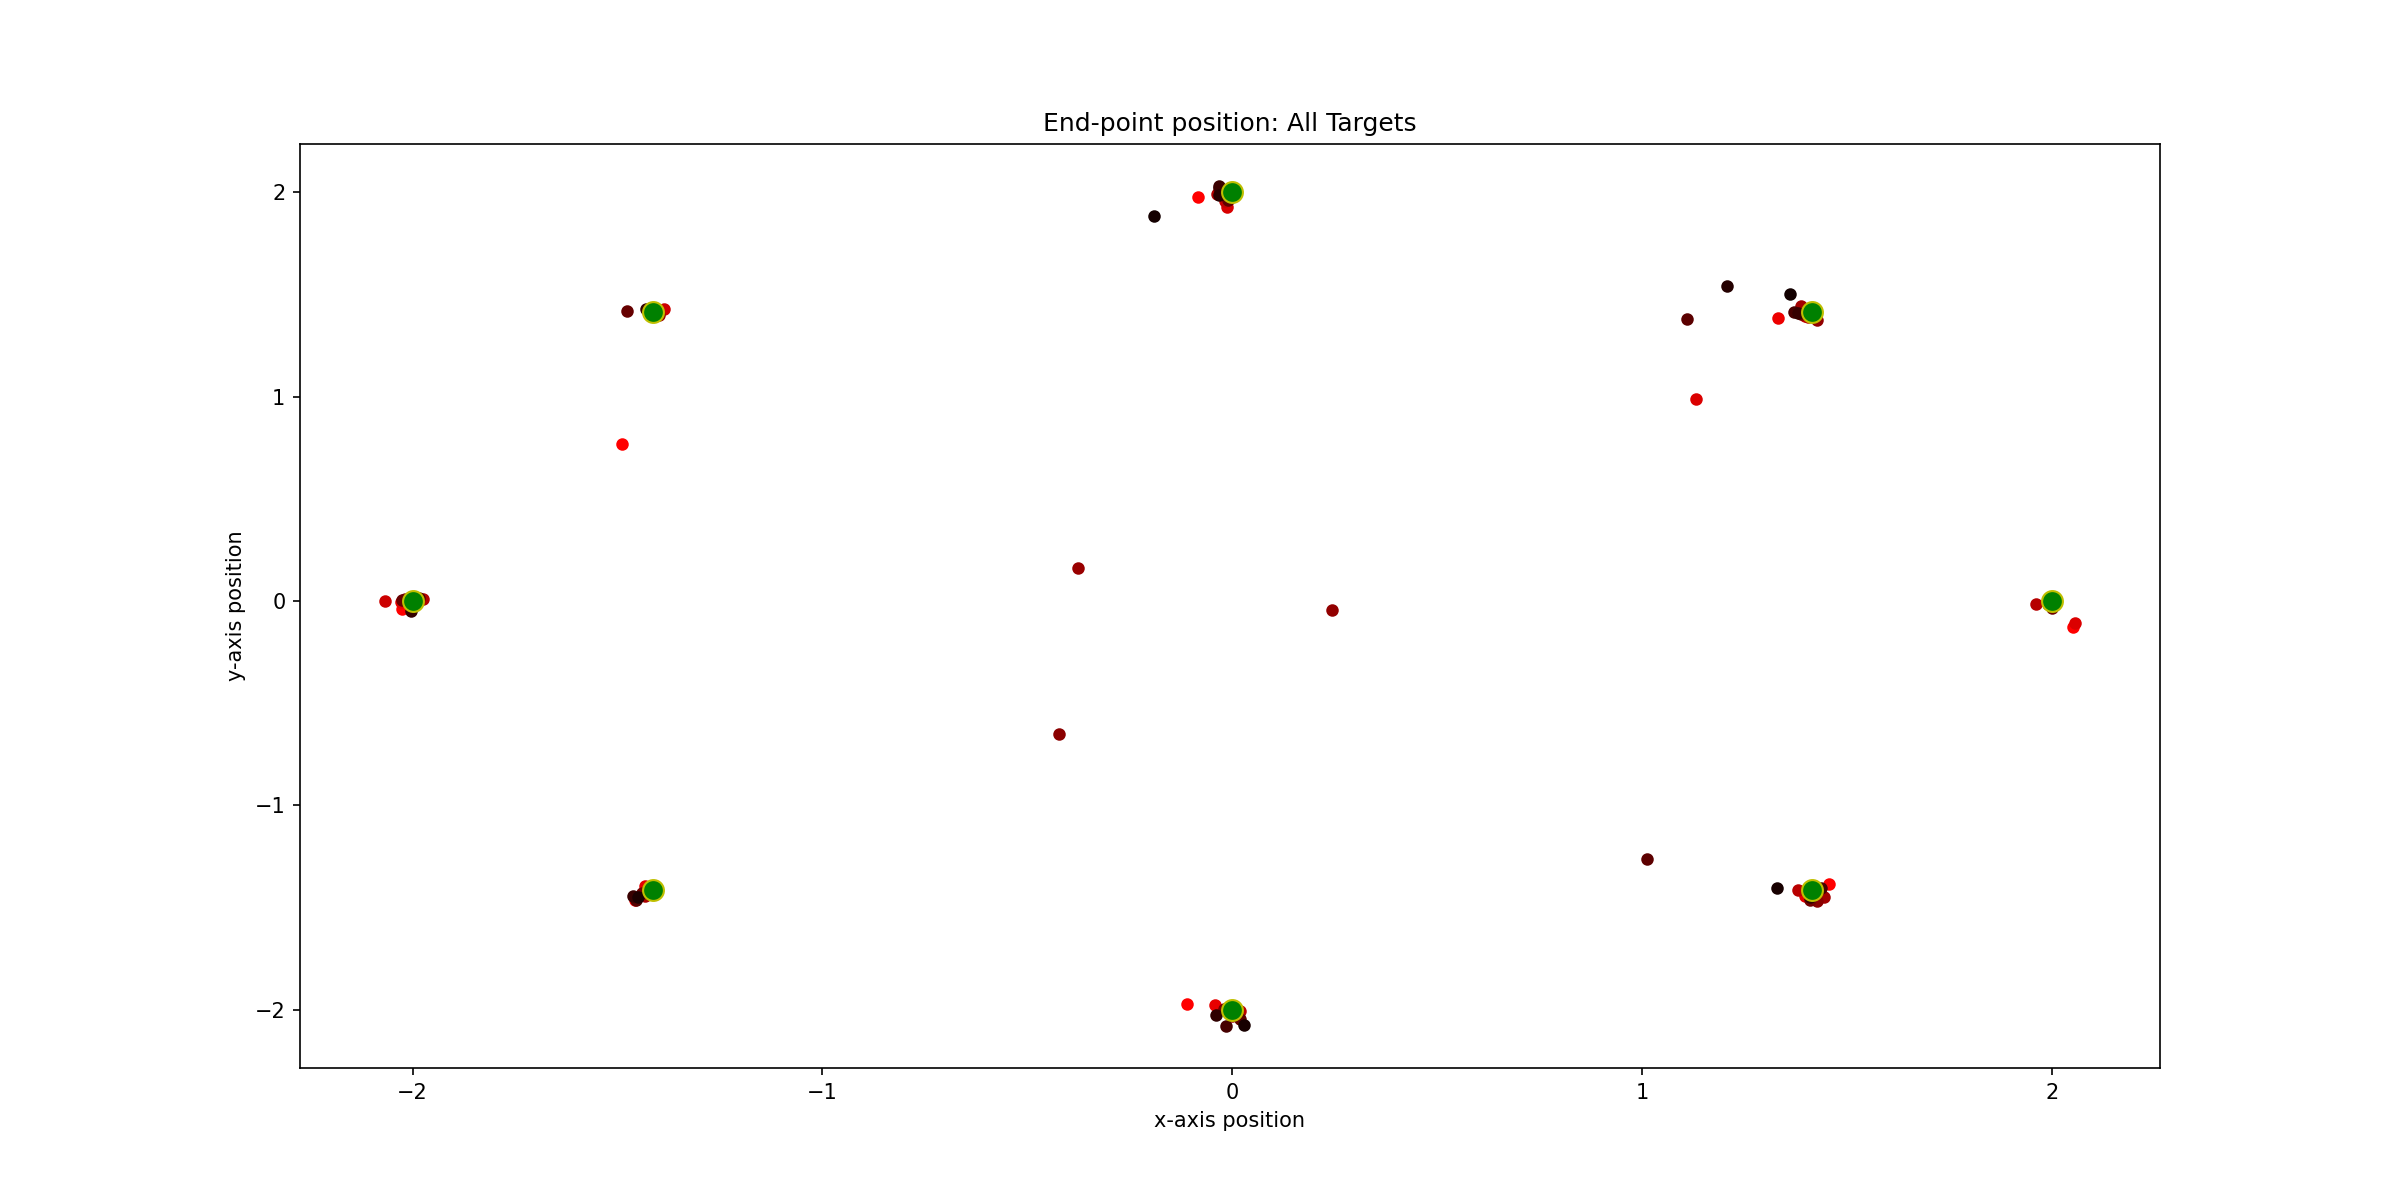
\includegraphics[scale=0.2]{sujeto3/force/trayectorias_puntos}
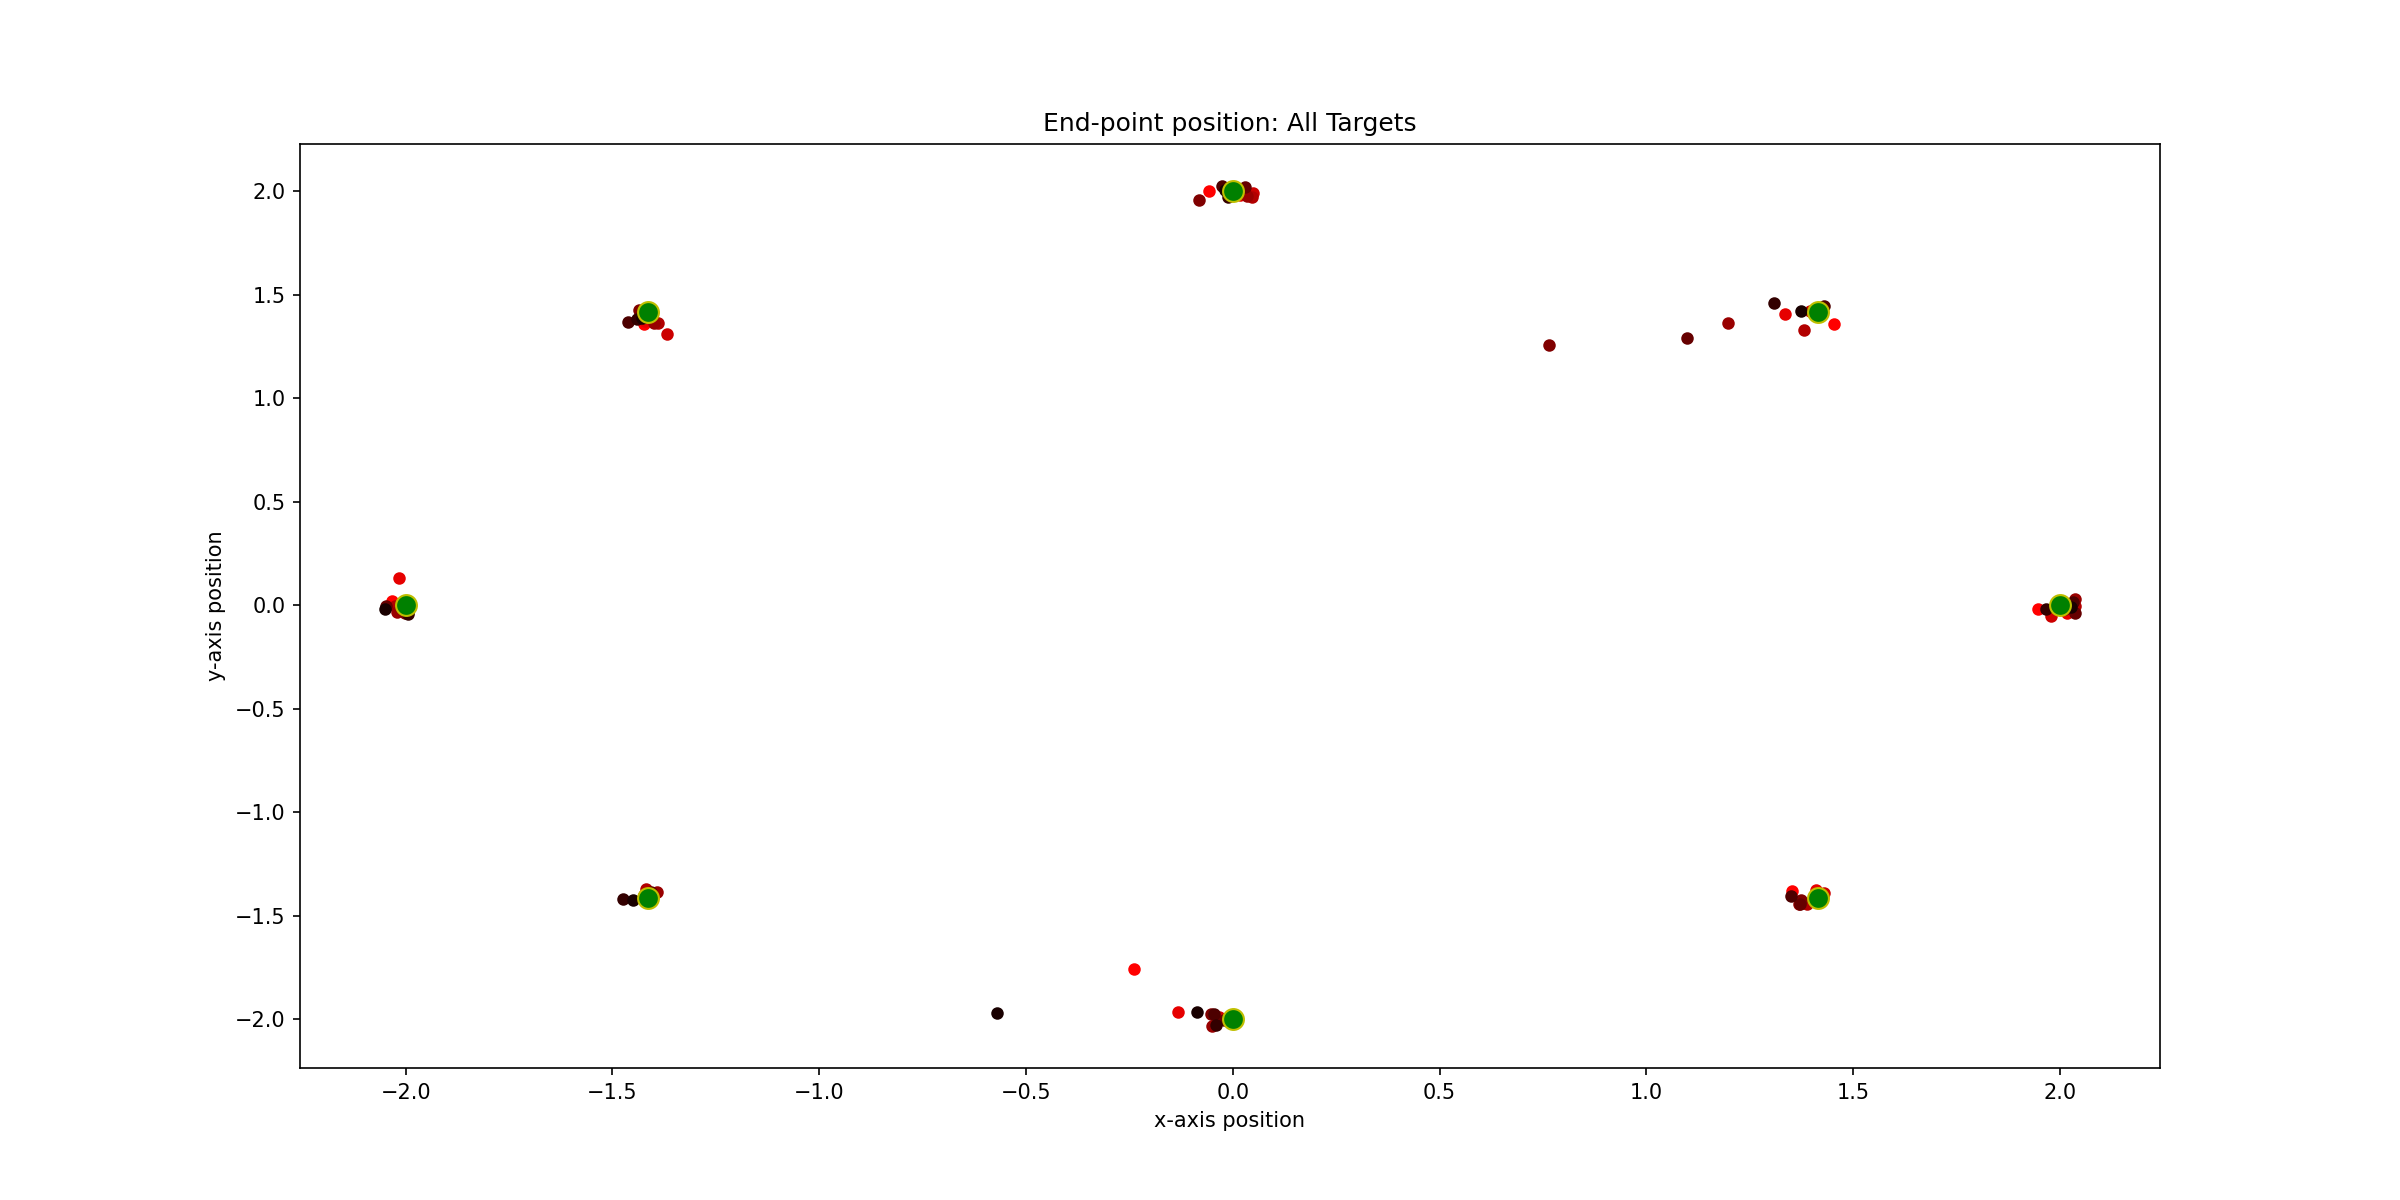
\includegraphics[scale=0.2]{sujeto5/force/trayectorias_puntos}

En cuanto a la evolución de los errores podemos ver que los sujetos 1,2 y 4 han extrapolado el aprendizaje del movimiento sin fuerza al movimiento con fuerza, y el error es cero o muy cercano a cero desde el primer momento:
\\
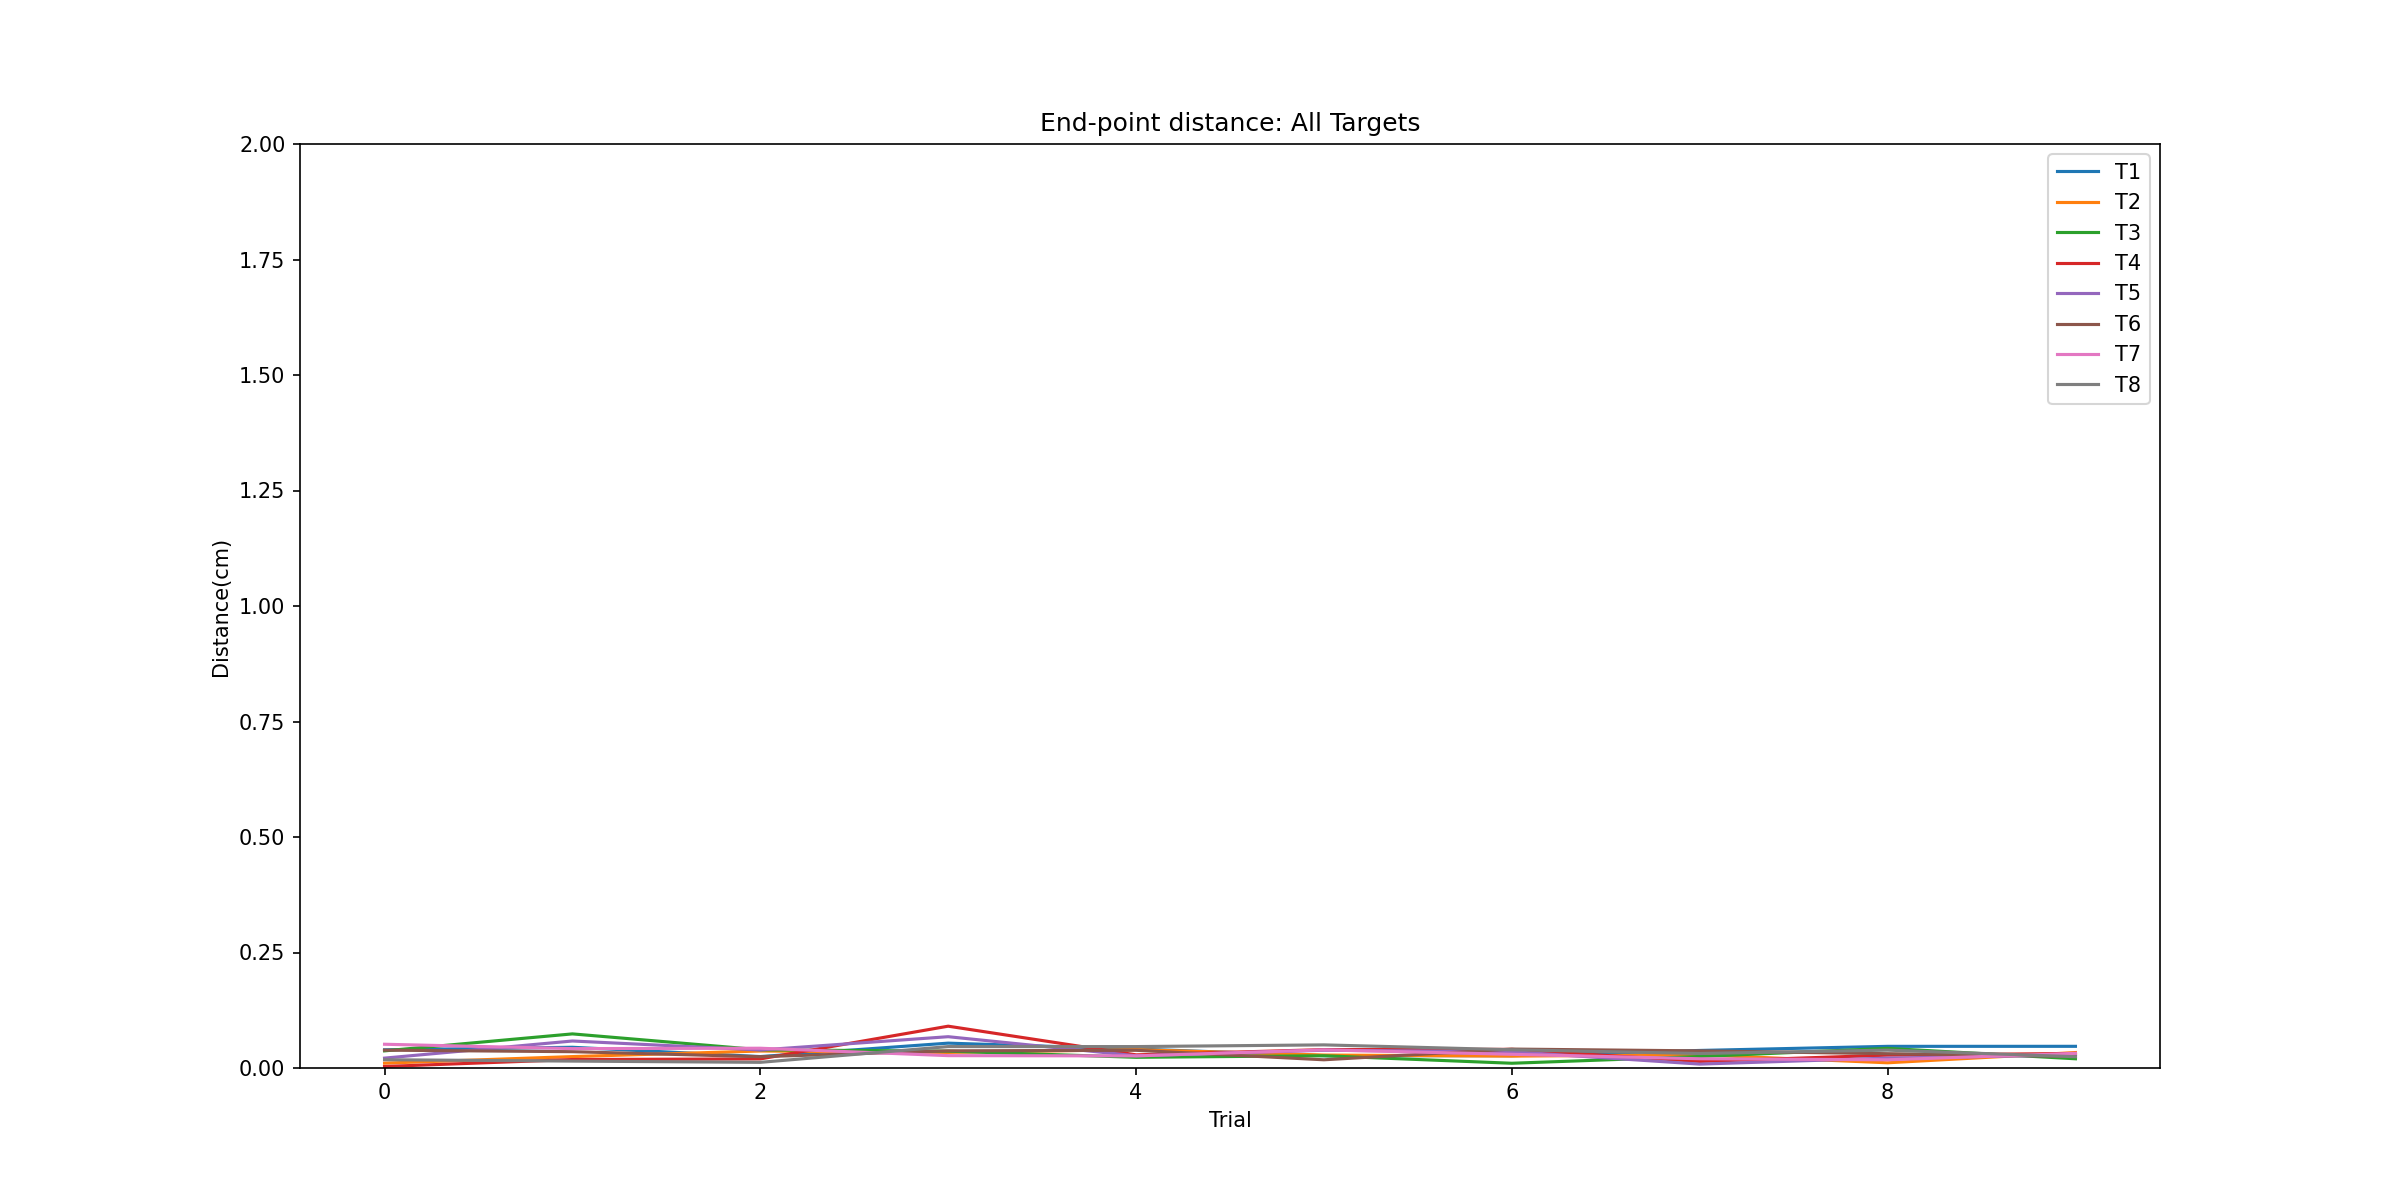
\includegraphics[scale=0.2]{sujeto1/force/evolution_distance}
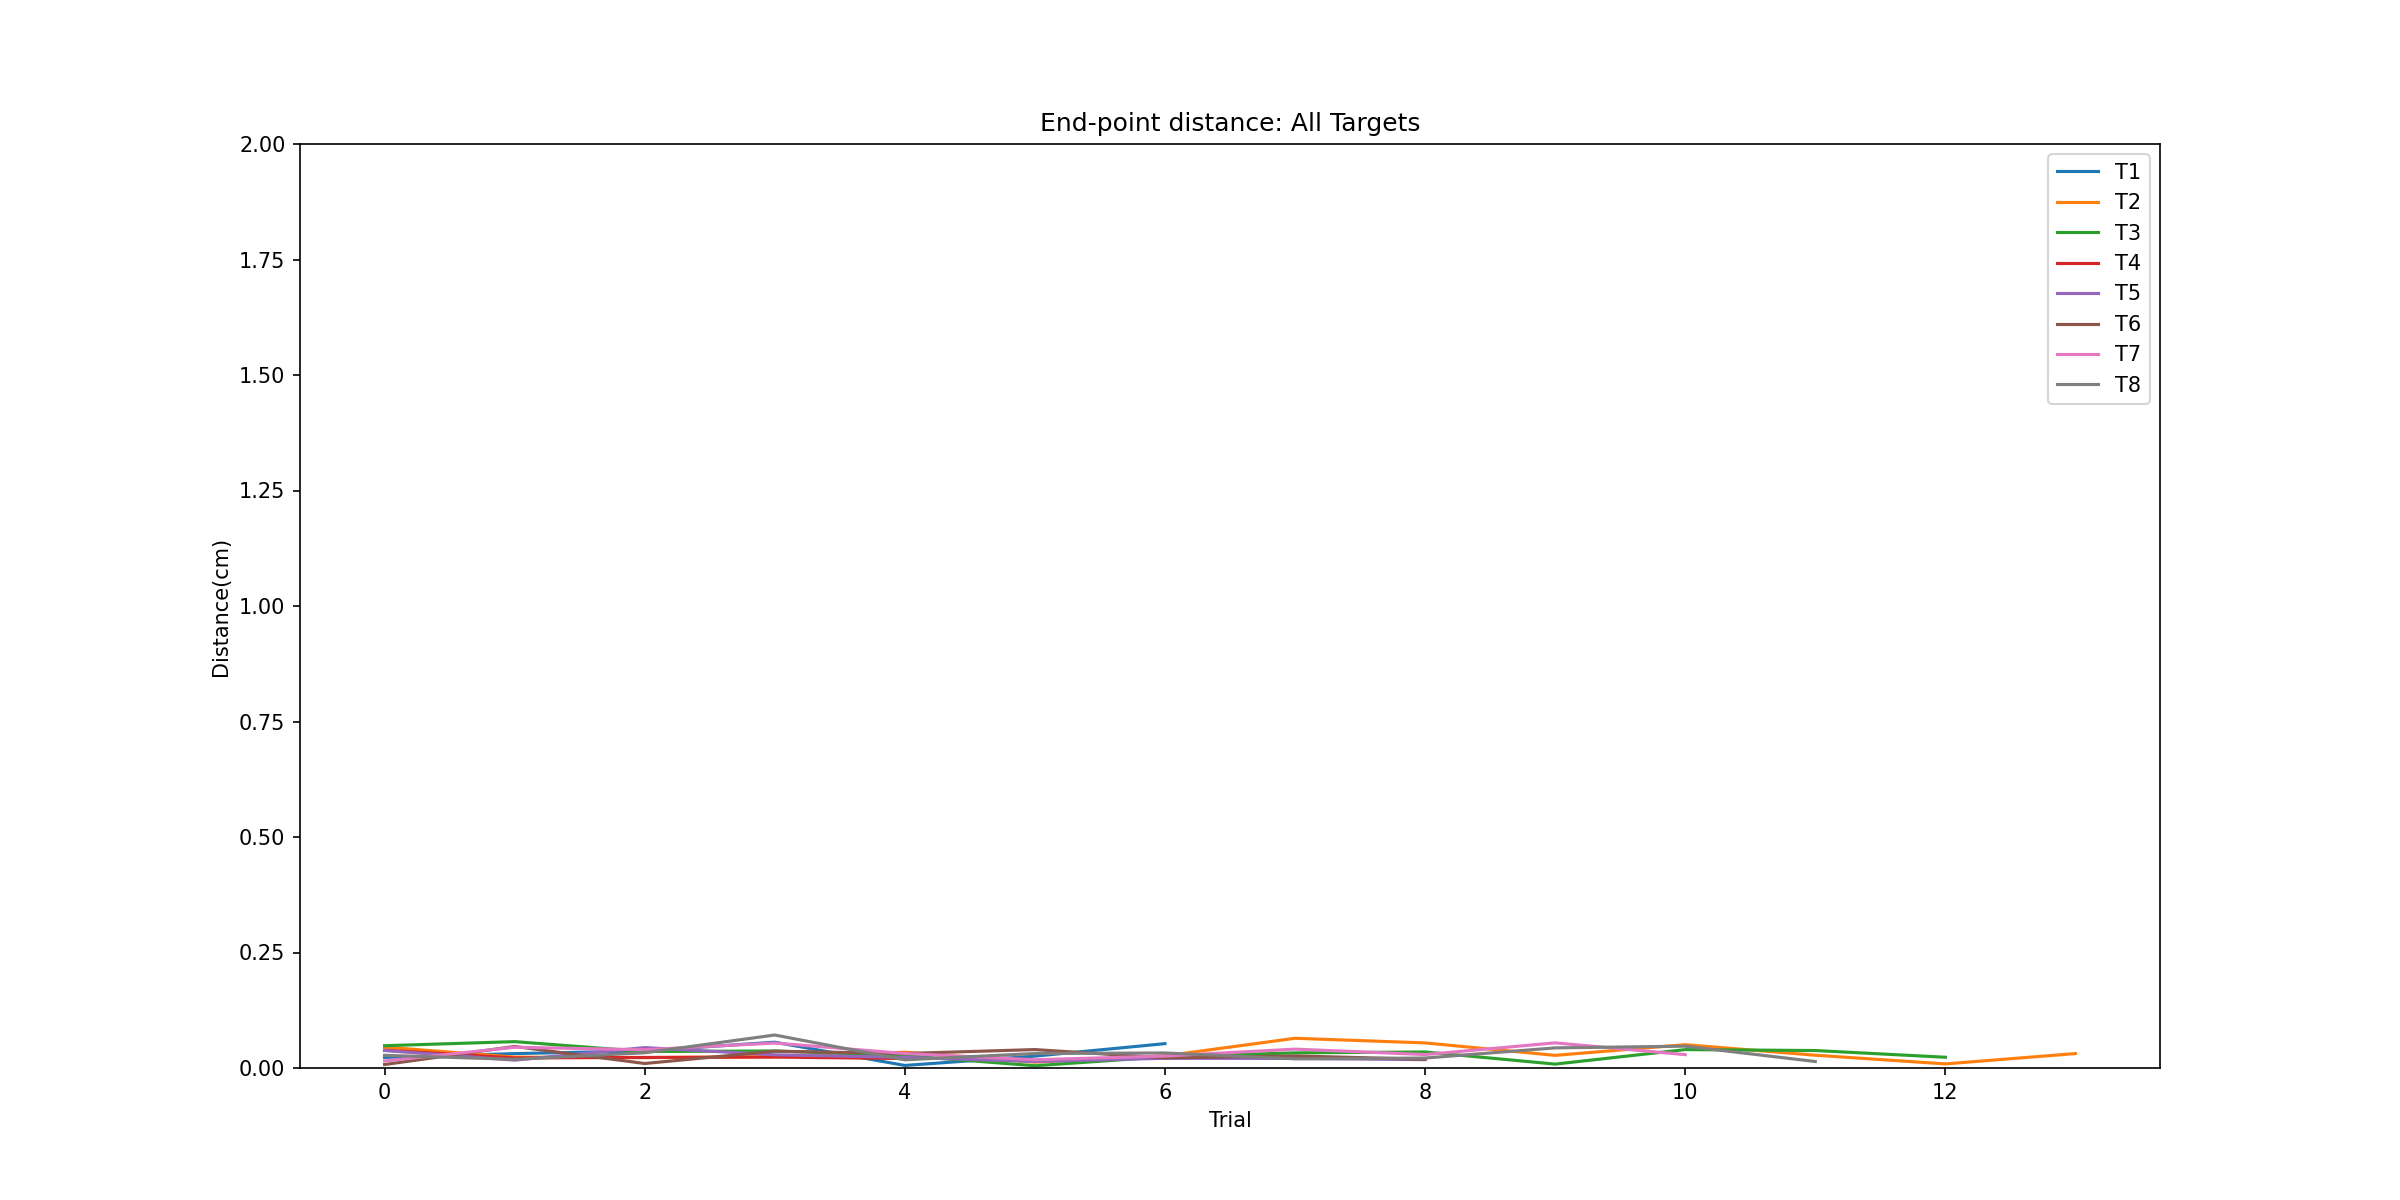
\includegraphics[scale=0.2]{sujeto2/force/evolution_distance}
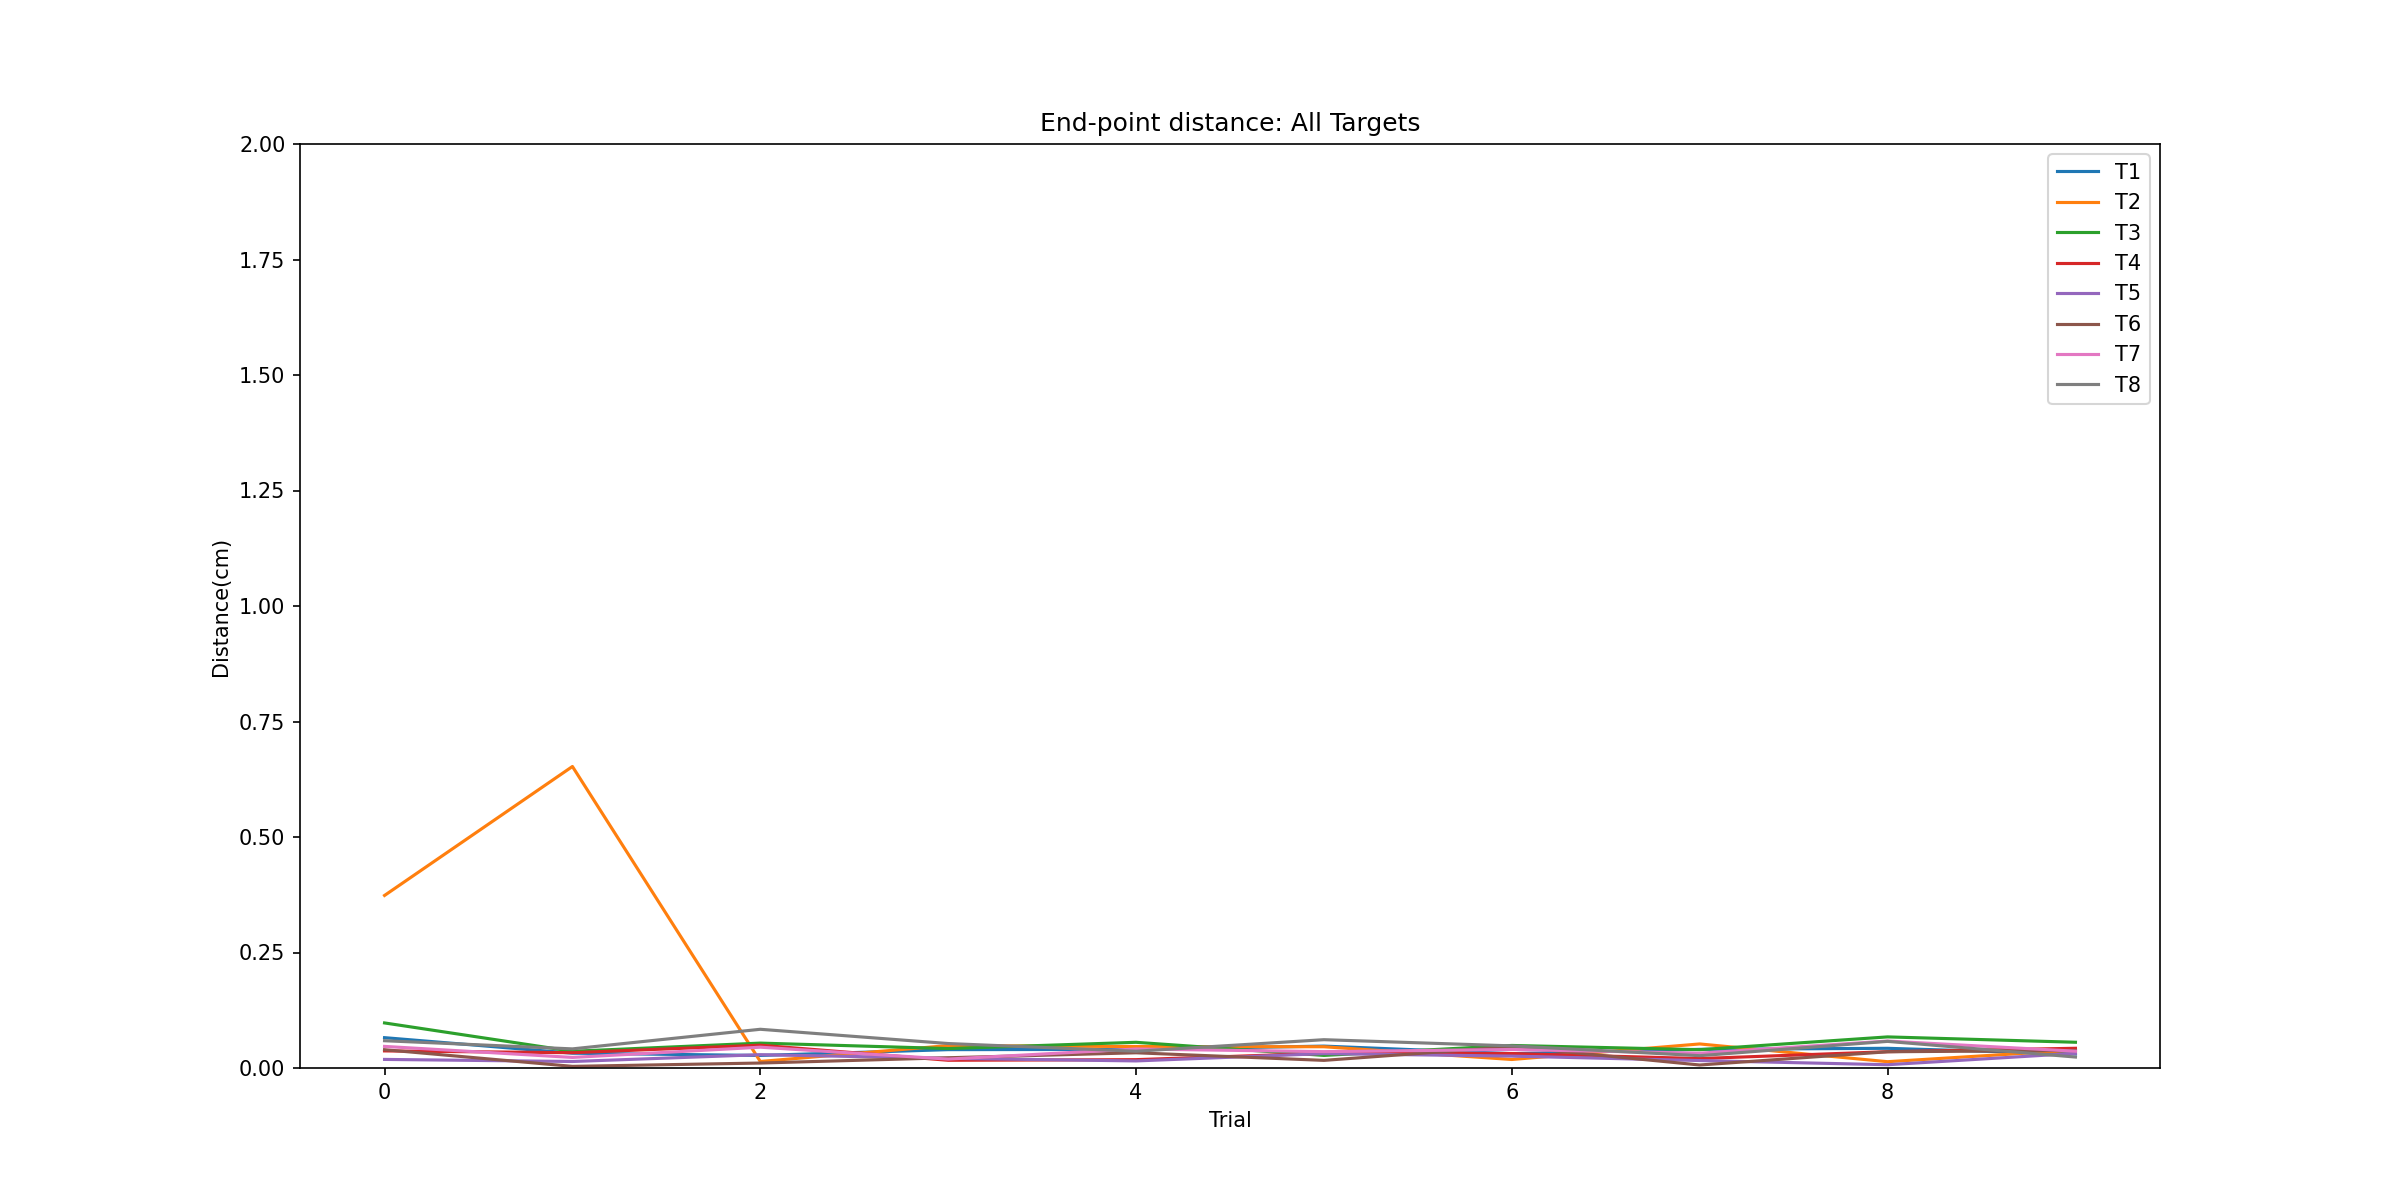
\includegraphics[scale=0.2]{sujeto4/force/evolution_distance}

El sujeto 5, a pesar de realizar movimentos muy largos también presenta una precisión bastante acertada, con unos errores, salvo en determinadas ocasiones, bastante bajos.

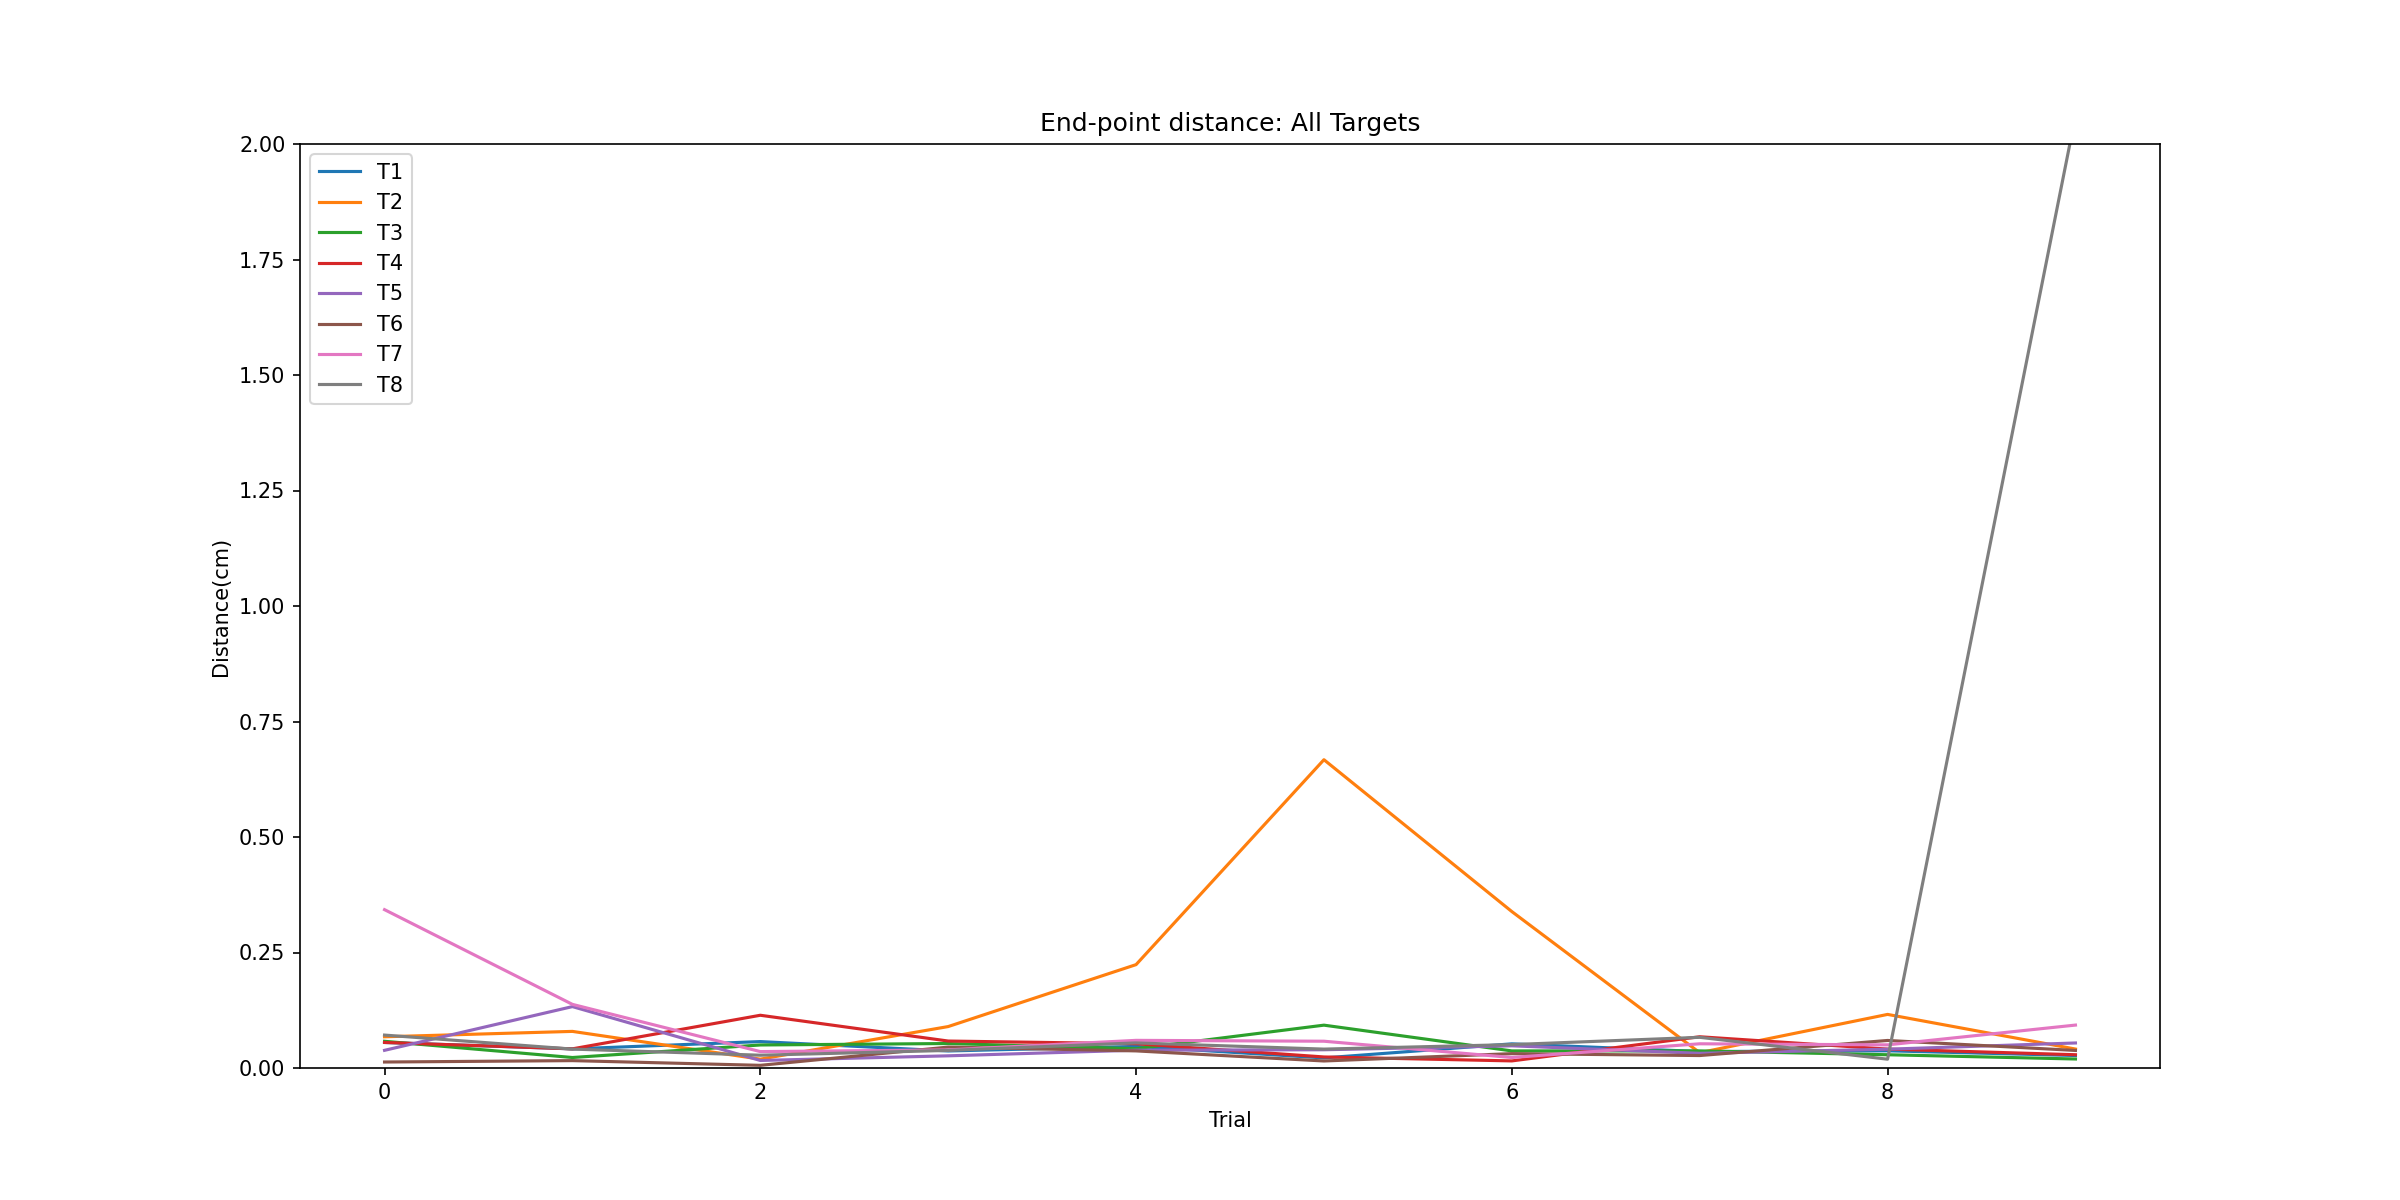
\includegraphics[scale=0.2]{sujeto5/force/evolution_distance}

El sujeto 3 presenta una distribución de los errores más errática, tanto estudiando los errores por target, como estudiando los errores totales.

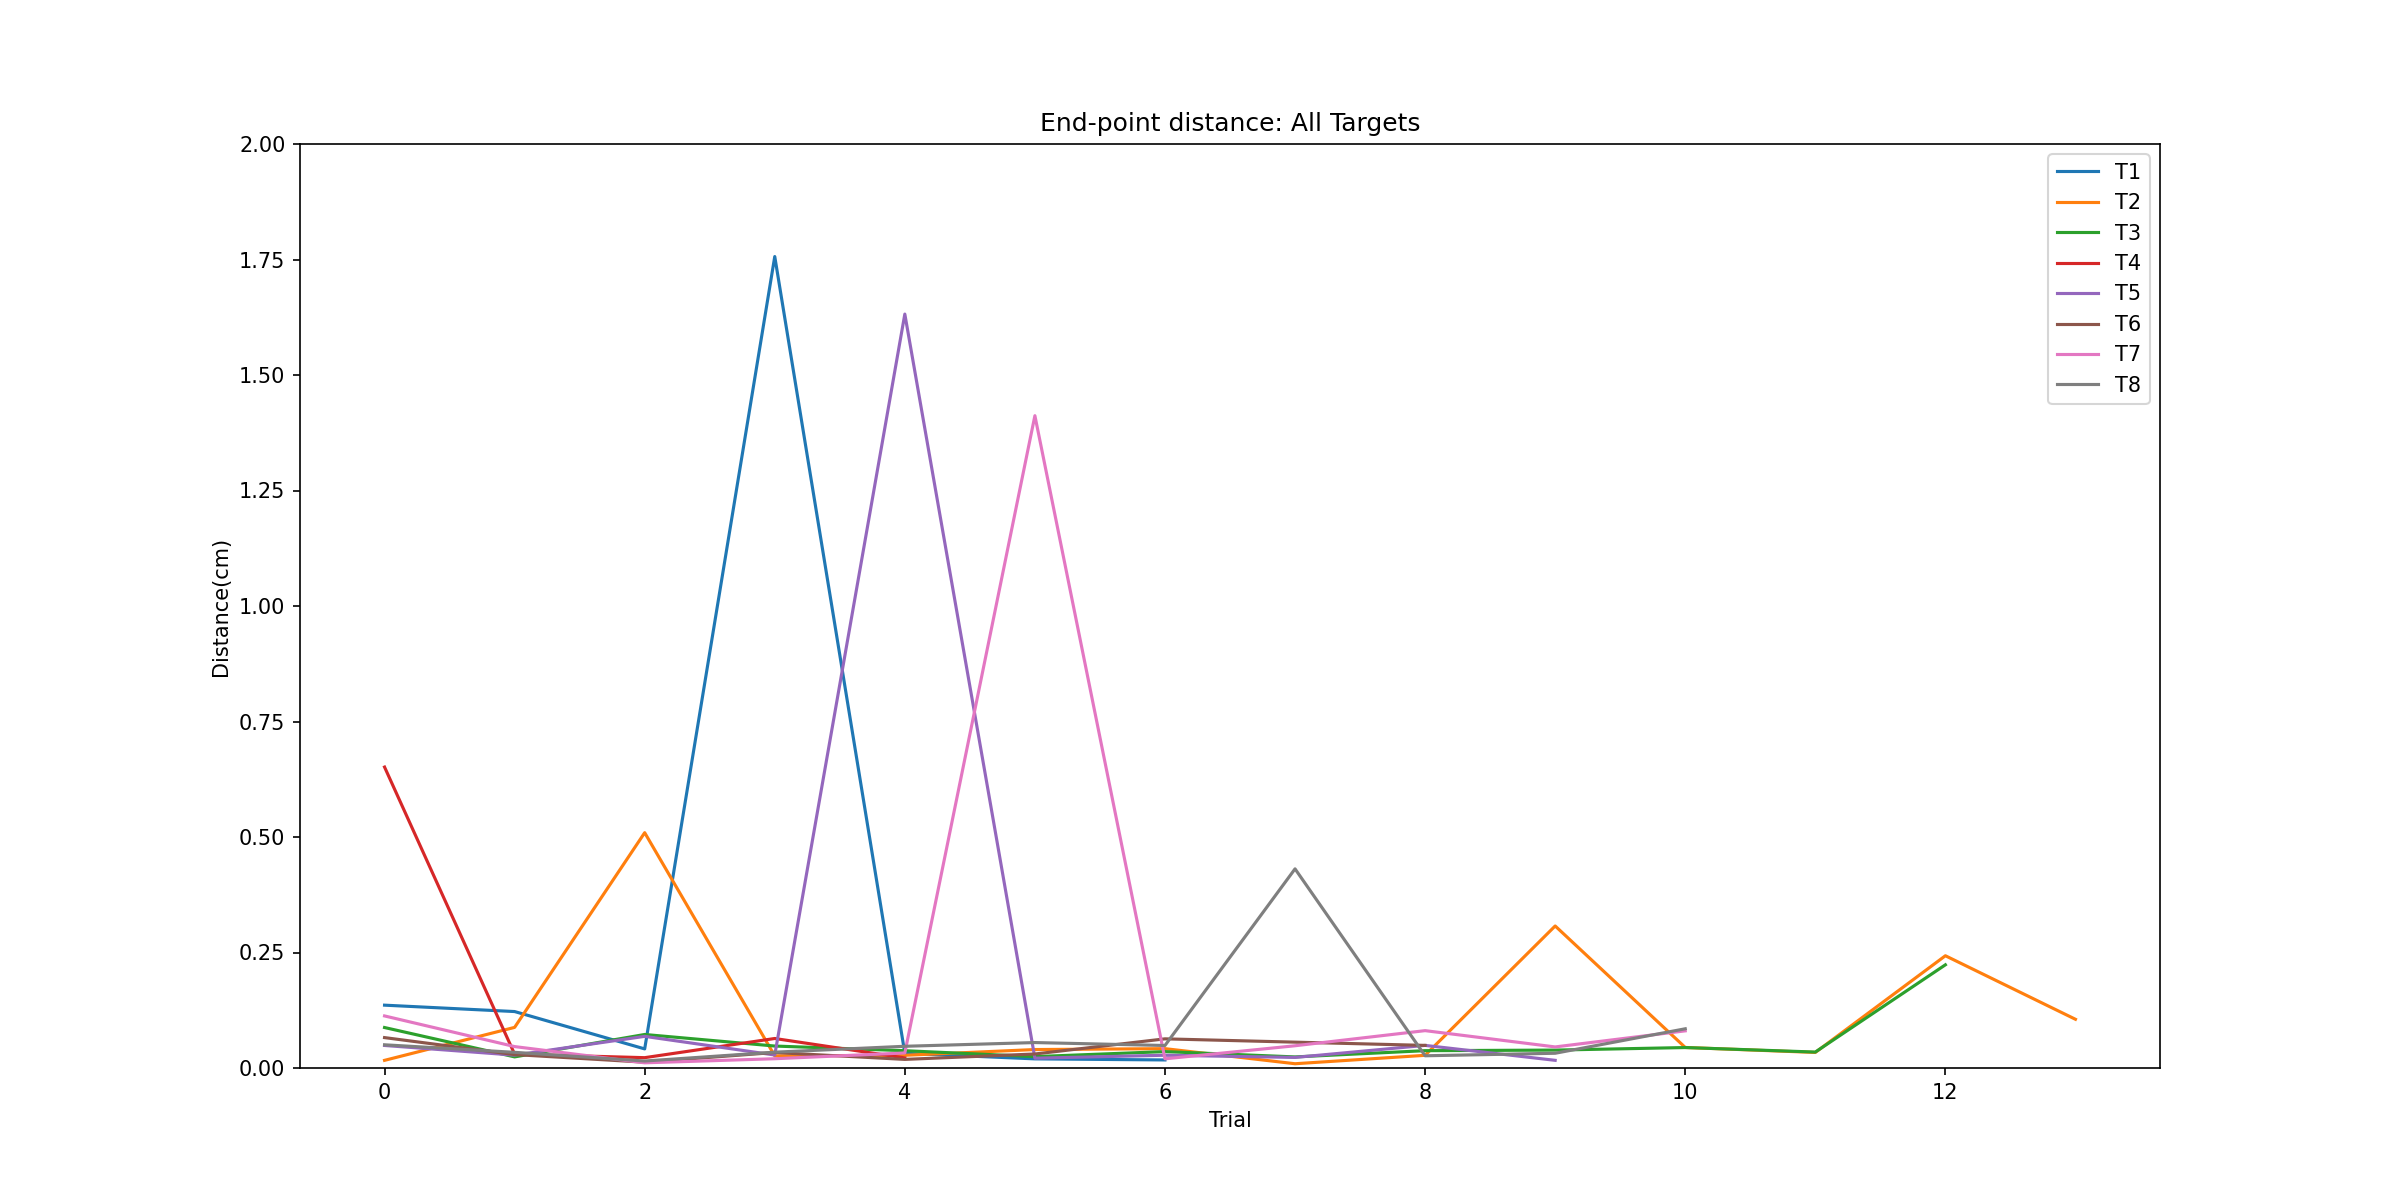
\includegraphics[scale=0.2]{sujeto3/force/evolution_distance}
\includegraphics[scale=0.4]{sujeto3/force/resumen_total}

Respecto a la rapidez en la ejecución del movimientos podemos observar resultados bastante similares entre los sujetos, siendo el sujeto 3 algo más lento que los demás. Sorprenden quizá los resultados del sujeto 5, quien, a pesar de hacer las trayectorias más largas, tiene unos tiempos de ejecución similares a los demás y mejores que los del otro sujeto mayor de 60 años. La mayor curva de aprendizaje se puede ver en el sujeto 4.

\includegraphics[scale=0.2]{sujeto1/force/evolution_time}
\includegraphics[scale=0.2]{sujeto2/force/evolution_time}
\includegraphics[scale=0.2]{sujeto3/force/evolution_time}
\includegraphics[scale=0.2]{sujeto4/force/evolution_time}
\includegraphics[scale=0.2]{sujeto5/force/evolution_time}


\subsubsection{Sin fuerza y sin cursor}

Respecto a las trayectorias podemos ver que, otra vez, es el sujeto 5 el que tiene las trayectorias más dispersas.

\includegraphics[scale=0.2]{sujeto1/no_force_no_cursor/trayectorias}
\includegraphics[scale=0.2]{sujeto2/no_force_no_cursor/trayectorias}
\includegraphics[scale=0.2]{sujeto3/no_force_no_cursor/trayectorias}
\includegraphics[scale=0.2]{sujeto4/no_force_no_cursor/trayectorias}
\includegraphics[scale=0.2]{sujeto5/no_force_no_cursor/trayectorias}

Y respecto a la distribución de puntos finales, los sujetos jóvenes tienen otra vez resultados más precisos que los sujetos mayores.

Sujetos jóvenes:
\\
\includegraphics[scale=0.2]{sujeto1/no_force_no_cursor/trayectorias_puntos}
\includegraphics[scale=0.2]{sujeto2/no_force_no_cursor/trayectorias_puntos}
\includegraphics[scale=0.2]{sujeto4/no_force_no_cursor/trayectorias_puntos}

Sujetos mayores de 60 años:
\\
\includegraphics[scale=0.2]{sujeto3/no_force_no_cursor/trayectorias_puntos}
\includegraphics[scale=0.2]{sujeto5/no_force_no_cursor/trayectorias_puntos}

Si estudiamos ahora la evolución de los errores en el tiempo podemos ver que en los sujetos jóvenes los errores se mantienen principalmente por debajo de $0.5$, mientras que en los sujetos mayores están por debajo de $0.75-1$. Respecto a las curvas de aprendizaje podemos ver que en los sujetos 1 y 4 (jóvenes, en orden) los resultados al final son algo mejores que los resultados al principio. Es interesante remarcar que en el otro sujeto joven (en orden aleatorio) no se ve ese aprendizaje, ni siquiera en los targets en los que hay más iteraciones (14). En los sujetos mayores observamos algo parecido: los resultados del sujeto 5 son algo mejores al final que al principio, salvo los dos últimos targets (tal vez por el cansancio); mientras que en el sujeto 3 podemos observar que los mejores resultados los tienen los targets con menos iteraciones, y que los targets con más iteraciones no mejoran los resultados.

\includegraphics[scale=0.2]{sujeto1/no_force_no_cursor/evolution_distance}
\includegraphics[scale=0.2]{sujeto2/no_force_no_cursor/evolution_distance}
\includegraphics[scale=0.2]{sujeto3/no_force_no_cursor/evolution_distance}
\includegraphics[scale=0.2]{sujeto4/no_force_no_cursor/evolution_distance}
\includegraphics[scale=0.2]{sujeto5/no_force_no_cursor/evolution_distance}

Si estudiamos ahora la evolución respecto al tiempo vemos que en este caso no podemos obtener mucha información de las gráficas, pues en casi ningún punto los sujetos han podido terminar el movimiento a tiempo.

\includegraphics[scale=0.2]{sujeto1/no_force_no_cursor/evolution_time}
\includegraphics[scale=0.2]{sujeto2/no_force_no_cursor/evolution_time}
\includegraphics[scale=0.2]{sujeto3/no_force_no_cursor/evolution_time}
\includegraphics[scale=0.2]{sujeto4/no_force_no_cursor/evolution_time}
\includegraphics[scale=0.2]{sujeto5/no_force_no_cursor/evolution_time}

\subsubsection{Con fuerza y sin cursor}

Respecto a las trayectorias podemos ver que, esta vez, los que realizan las trayectorias más largas son el sujeto 1 y el 5 (en la fase de fuerza y cursor eran el sujeto 3 y el 5). En la gráfica del sujeto 4 podemos ver claramente como se realiza el aprendizaje del movimiento, pues en las primeras trayectorias en cada punto se puede observar el efecto de la fuerza, que en las iteraciones siguientes se corrije para dar lugar a trayectorias más rectas.

\includegraphics[scale=0.2]{sujeto1/force_no_cursor/trayectorias}
\includegraphics[scale=0.2]{sujeto2/force_no_cursor/trayectorias}
\includegraphics[scale=0.2]{sujeto3/force_no_cursor/trayectorias}
\includegraphics[scale=0.2]{sujeto4/force_no_cursor/trayectorias}
\includegraphics[scale=0.2]{sujeto5/force_no_cursor/trayectorias}


En la distribución de puntos finales podemos ver que el más preciso de todos los sujetos es el 4, y el menos el 3. Los sujetos 1 y 2 tienen un desempeño similar, mientras que el del 5 es algo peor.

\includegraphics[scale=0.2]{sujeto1/force_no_cursor/trayectorias_puntos}
\includegraphics[scale=0.2]{sujeto2/force_no_cursor/trayectorias_puntos}
\includegraphics[scale=0.2]{sujeto3/force_no_cursor/trayectorias_puntos}
\includegraphics[scale=0.2]{sujeto4/force_no_cursor/trayectorias_puntos}
\includegraphics[scale=0.2]{sujeto5/force_no_cursor/trayectorias_puntos}

Vamos ahora a analizar la evolución de los errores en cada target. Podemos ver que el mejor es el sujeto 5, que sigue manteniéndose por debajo de 0.5, y experimenta un ligero pero no muy claro aprendizaje. Las gráficas del sujeto 1 (en orden) y el 2 (aleatorio) son parecidas, en el 1 podemos observar que los errores en las últimas iteraciones son algo menores, pero en el 2 vemos otra vez que los targets con más iteraciones (14) no tienen mejor desempeño. 

Respecto a los sujetos mayores vemos que aquí si hay más diferencia entre el sujeto 5 (en orden) y el sujeto 3 (aleatorio). Mientras que el sujeto 5 muestra cierto aprendizaje (salvo en T8) el sujeto 3 tiene un comportamiento más errático y con mayores errores.

\includegraphics[scale=0.2]{sujeto1/force_no_cursor/evolution_distance}
\includegraphics[scale=0.2]{sujeto2/force_no_cursor/evolution_distance}
\includegraphics[scale=0.2]{sujeto3/force_no_cursor/evolution_distance}
\includegraphics[scale=0.2]{sujeto4/force_no_cursor/evolution_distance}
\includegraphics[scale=0.2]{sujeto5/force_no_cursor/evolution_distance}

Respecto a la evolución de la velocidad en este caso volvemos a no poder extraer mucha información, pues en casi ningún punto los sujetos han podido realizar el movimiento a tiempo. En todo caso vuelven a ser los sujetos jóvenes los que tienen mejores tiempos.

\includegraphics[scale=0.2]{sujeto1/force_no_cursor/evolution_time}
\includegraphics[scale=0.2]{sujeto2/force_no_cursor/evolution_time}
\includegraphics[scale=0.2]{sujeto3/force_no_cursor/evolution_time}
\includegraphics[scale=0.2]{sujeto4/force_no_cursor/evolution_time}
\includegraphics[scale=0.2]{sujeto5/force_no_cursor/evolution_time}

\subsection{Análisis de diferentes fases entre el mismo individuo}

Vamos ahora a estudiar la evolución de cada sujeto a través de las diferentes fases. De esta forma queremos analizar cómo ha afectado la fuerza que hemos aplicado al dispositivo, y si el sujeto extrapola el aprendizaje realizado en una fase a otra.

Para ello vamos a estudiar principalmente las trayectorias y los puntos finales, para ver los movimientos realizados y la precisión y exactitud de esos movimientos.

\subsubsection{Sujeto 1}

En la primera fase podemos ver que los movimientos son muy precisos y exactos (a partir de T3 no hay errores), y las trayectorias, salvo las primeras en cada target, son líneas rectas, especialmente las de los targets T1, T3, T5, T7, que a priori son las más fáciles.

En la segunda fase vemos que se extrapola completamente el aprendizaje realizado en la primera fase, pues no hay errores desde el principio, por lo que la precisión es incluso mayor. Las trayectorias sin embargo son algo más largas, y los movimientos más cortos se producen en los targets T1 y T5, lo que a priori también tiene sentido pues es la dirección en la que estamos aplicando la fuerza. Respecto al tiempo de ejecución las dos fases tienen resultados parecidos.

En la tercera fase, ahora sin retroalimentación del cursor, podemos ver que baja la precisión de los movimientos pero las trayectorias, salvo las primeras de cada target, son líneas rectas.

En la cuarta fase vemos que la precisión baja algo más y tiende a desplazarse en el sentido de la fuerza, especialmente en los targets en los que el movimiento es en el sentido de la fuerza. En las trayectorias se observa ahora más el efecto de la fuerza, y no podemos apreciar claramente que se efecto se contrarreste cuando realizamos más iteraciones.

\includegraphics[scale=0.2]{sujeto1/no_force/trayectorias}
\includegraphics[scale=0.2]{sujeto1/no_force/trayectorias_puntos}

\includegraphics[scale=0.2]{sujeto1/force/trayectorias}
\includegraphics[scale=0.2]{sujeto1/force/trayectorias_puntos}

\includegraphics[scale=0.2]{sujeto1/no_force_no_cursor/trayectorias}
\includegraphics[scale=0.2]{sujeto1/no_force_no_cursor/trayectorias_puntos}

\includegraphics[scale=0.2]{sujeto1/force_no_cursor/trayectorias}
\includegraphics[scale=0.2]{sujeto1/force_no_cursor/trayectorias_puntos}


\subsubsection{Sujeto 2}

En la primera fase podemos ver que el sujeto 1 realiza correctamente los movimientos desde la primera iteración. Además las trayectorias son bastante rectas.

En la segunda fase vemos que sigue manteniendo un 100 por 100 de precisión, aunque las trayectorias ahora son un poco más largas, especialmente en T6 y T7.

En la tercera fase podemos observar que baja la precisión, pero las trayectorias siguen siendo rectas. 

En la cuarta fase los resultados son parecidos a la tercera, por lo que podemos ver que la fuerza que hemos aplicado no ha afectado a la precisión de los movimientos, aunque sí afecta ligeramente a las trayectorias realizadas, que se vuelven algo menos definidas. Las trayectorias más definidas vuelven a ser las que se realizan en la dirección de la fuerza.

\includegraphics[scale=0.2]{sujeto2/no_force/trayectorias}
\includegraphics[scale=0.2]{sujeto2/no_force/trayectorias_puntos}

\includegraphics[scale=0.2]{sujeto2/force/trayectorias}
\includegraphics[scale=0.2]{sujeto2/force/trayectorias_puntos}

\includegraphics[scale=0.2]{sujeto2/no_force_no_cursor/trayectorias}
\includegraphics[scale=0.2]{sujeto2/no_force_no_cursor/trayectorias_puntos}\\

\includegraphics[scale=0.2]{sujeto2/force_no_cursor/trayectorias}
\includegraphics[scale=0.2]{sujeto2/force_no_cursor/trayectorias_puntos}

\subsubsection{Sujeto 3}

En la primera y la segunda fase vemos unos resultados muy parecidos en cuanto a precisión, aunque respecto a las trayectorias podemos ver que en la fase en la que aplicamos la fuerza están desviadas en el sentido de la fuerza. Aún así esto no afecta a la precisión ni a la velocidad del movimiento.

Respecto a las fases en las que no se muestra el cursor podemos ver que los puntos finales cuando aplicamos fuerza están algo desplazados en la dirección de la fuerza, mientras que al no aplicar fuerza se reparten aleatoriamente alrededor del punto objetivo. Las trayectorias también son algo menos claras al aplicar fuerza. Aún así los resultados son parecidos en términos de exactitud y tiempo.

\includegraphics[scale=0.2]{sujeto3/no_force/trayectorias}
\includegraphics[scale=0.2]{sujeto3/no_force/trayectorias_puntos}

\includegraphics[scale=0.2]{sujeto3/force/trayectorias}
\includegraphics[scale=0.2]{sujeto3/force/trayectorias_puntos}

\includegraphics[scale=0.2]{sujeto3/no_force_no_cursor/trayectorias}
\includegraphics[scale=0.2]{sujeto3/no_force_no_cursor/trayectorias_puntos}

\includegraphics[scale=0.2]{sujeto3/force_no_cursor/trayectorias}
\includegraphics[scale=0.2]{sujeto3/force_no_cursor/trayectorias_puntos}


\subsubsection{Sujeto 4}

El sujeto 4 es el que presenta los resultados más parecidos entre fases. 

Tanto en la fase 1 como en la 2 los movimientos son casi 100 por 100 precisos y las trayectorias son líneas rectas, exceptuando la primera iteración en cada target.

En las fases en las que no hay realimentación del cursor los resultados son muy parecidos, con una precisión casi similar en la fase sin fuerza y con fuerza. En las trayectorias tampoco podemos observar una influencia muy clara de la fuerza.

Por lo tanto en el sujeto 4 no hemos obtenido resultados diferentes que indiquen que tiene sentido diferencias estos dos tipos de movimientos (con fuerza y sin fuerza).


\includegraphics[scale=0.2]{sujeto4/no_force/trayectorias}
\includegraphics[scale=0.2]{sujeto4/no_force/trayectorias_puntos}\

\includegraphics[scale=0.2]{sujeto4/force/trayectorias}
\includegraphics[scale=0.2]{sujeto4/force/trayectorias_puntos}

\includegraphics[scale=0.2]{sujeto4/no_force_no_cursor/trayectorias}
\includegraphics[scale=0.2]{sujeto4/no_force_no_cursor/trayectorias_puntos}\\

\includegraphics[scale=0.2]{sujeto4/force_no_cursor/trayectorias}
\includegraphics[scale=0.2]{sujeto4/force_no_cursor/trayectorias_puntos}


\subsubsection{Sujeto 5}

En el sujeto 5 es en el que podemos observar mejor los efectos de la fuerza, aunque solo en las trayectorias.

En la fase 1 podemos observar que se produce un aprendizaje en los dos primeros targets, que luego se extrapola a los targets siguientes. En la fase con fuerza ese aprendizaje se extrapola en el primer target, en el segundo target vuelven a aparecer errores y luego se vuelve a conseguir una precisión bastante buena. Por tanto los resultados al final son muy parecidos entre fases. 

En cuanto a las trayectorias se puede apreciar con claridad los efectos de la fuerza, pues los movimientos siguen el sentido de la fuerza y no se corrigen cuando se repite el movimiento más veces.

Respecto a las fases 3 y 4 los resultados vuelven a ser muy parecidos, con una precisión casi igual en las dos fases. Es interesante remarcar que las trayectorias curvas que se realizan en la fase 2 se suavizan bastante en la fase 4. 

\includegraphics[scale=0.2]{sujeto5/no_force/trayectorias}
\includegraphics[scale=0.2]{sujeto5/no_force/trayectorias_puntos}

\includegraphics[scale=0.2]{sujeto5/force/trayectorias}
\includegraphics[scale=0.2]{sujeto5/force/trayectorias_puntos}

\includegraphics[scale=0.2]{sujeto5/no_force_no_cursor/trayectorias}
\includegraphics[scale=0.2]{sujeto5/no_force_no_cursor/trayectorias_puntos}\\

\includegraphics[scale=0.2]{sujeto5/force_no_cursor/trayectorias}
\includegraphics[scale=0.2]{sujeto5/force_no_cursor/trayectorias_puntos}

\chapter{Discusion y conclusiones}
Resumen comparación entre sujetos

\chapter{Bibliografía}
https://quasardynamics.com/dispositivos-hapticos-la-realidad-virtual/
https://es.3dsystems.com/haptics-devices/touch
\end{document}
